%%% Copyright (C) 2017 Vincent Goulet
%%%
%%% Ce fichier et tous les fichiers .tex ou .Rnw dont la racine est
%%% mentionnée dans les commandes \include ci-dessous font partie du
%%% projet «Programmer avec R»
%%% http://github.com/vigou3/programmer-avec-r
%%%
%%% Cette création est mise à disposition selon le contrat
%%% Attribution-Partage dans les mêmes conditions 4.0
%%% International de Creative Commons.
%%% http://creativecommons.org/licenses/by-sa/4.0/

\documentclass[letterpaper,11pt,x11names,english,french]{memoir}
  \usepackage{natbib,url}
  \usepackage{babel}
  \usepackage[autolanguage]{numprint}
  \usepackage{amsmath,amsthm}
  \usepackage[noae]{Sweave}
  \usepackage{framed}                  % env. snugshade*, oframed
  \usepackage[shortlabels]{enumitem}
  \usepackage[absolute]{textpos}       % éléments des pages de titre
  \usepackage{graphicx}
  \usepackage{relsize}                 % \smaller et al.
  \usepackage{manfnt}                  % \mantriangleright (puce)
  \usepackage{metalogo}                % \XeLaTeX logo
  \usepackage{applekeys}               % touches Mac
  \usepackage{dirtree}                 % arbre pour exercice sur \include
  \usepackage{fontawesome}             % icônes \fa*
  \usepackage{awesomebox}              % boites info, important, etc.
  \usepackage{answers}                 % exercices et solutions
  \usepackage{listings}                % code informatique
  \usepackage{pgf}                     % transparence pour couverture avant

  %%% =============================
  %%%  Informations de publication
  %%% =============================
  \title{Programmer avec R}
  \author{Vincent Goulet}
  \renewcommand{\year}{2017}
  \renewcommand{\month}{09-1a}
  \newcommand{\ISBN}{}
  \newcommand{\ghurl}{https://github.com/vigou3/programmer-avec-r/}

  %%% ===================
  %%%  Style du document
  %%% ===================

  %% Polices de caractères
  \usepackage{fontspec}
  \usepackage{unicode-math}
  \defaultfontfeatures{Scale=0.92}
  \setmainfont[Ligatures=TeX,Numbers=OldStyle]{Lucida Bright OT}
  \setmathfont{Lucida Bright Math OT}
  \setmonofont{Lucida Grande Mono DK}
  \setsansfont[Scale=1.0,Numbers=OldStyle]{Myriad Pro}
  \newfontfamily\fullcaps[Letters=Uppercase,Numbers=Uppercase]{Myriad Pro}
  \usepackage[babel=true]{microtype}
  \usepackage{icomma}

  %% Couleurs
  \usepackage{xcolor}
  \definecolor{comments}{rgb}{0.7,0,0}      % commentaires
  \definecolor{link}{rgb}{0,0.4,0.6}        % liens internes
  \definecolor{url}{rgb}{0.6,0,0}           % liens externes
  \definecolor{citation}{rgb}{0,0.5,0}      % citations
  \definecolor{codebg}{named}{LightYellow1} % fond code R
  \definecolor{prob}{named}{orange}         % encadrés «problème»
  \definecolor{rouge}{rgb}{0.85,0,0.07} % rouge bandeau identitaire
  \definecolor{or}{rgb}{1,0.8,0}        % or bandeau identitaire

  %% Hyperliens
  \usepackage{hyperref}
  \hypersetup{%
    pdfauthor = \theauthor,
    pdftitle = \thetitle,
    colorlinks = {true},
    linktocpage = {true},
    urlcolor = {url},
    linkcolor = {link},
    citecolor = {citation},
    pdfpagemode = {UseOutlines},
    pdfstartview = {Fit},
    bookmarksopen = {true},
    bookmarksnumbered = {true},
    bookmarksdepth = {subsubsection}}
  \setlength{\XeTeXLinkMargin}{1pt}

  %% Étiquettes de \autoref (redéfinitions compatibles avec babel).
  %% Attention! Les % à la fin des lignes sont importants sinon des
  %% blancs apparaissent dès que la commande \selectlanguage est
  %% utilisée... comme dans la bibliographie, par exemple.
  \addto\extrasfrench{%
    \def\appendixautorefname{annexe}%
    \def\figureautorefname{figure}%
    \def\exempleautorefname{exemple}%
    \def\exerciceautorefname{exercice}%
    \def\subfigureautorefname{figure}%
    \def\subsectionautorefname{section}%
    \def\subtableautorefname{tableau}%
    \def\tableautorefname{tableau}%
  }

  %% Table des matières (inspirée de classicthesis.sty)
  \renewcommand{\cftchapterleader}{\hspace{1.5em}}
  \renewcommand{\cftchapterafterpnum}{\cftparfillskip}
  \renewcommand{\cftsectionleader}{\hspace{1.5em}}
  \renewcommand{\cftsectionafterpnum}{\cftparfillskip}

  %% Titres des chapitres
  \chapterstyle{hangnum}
  \renewcommand{\chaptitlefont}{\normalfont\Huge\sffamily\bfseries\raggedright}

  %% Marges, entêtes et pieds de page
  \setlength{\marginparsep}{7mm}
  \setlength{\marginparwidth}{13mm}
  \setlength{\headwidth}{\textwidth}
  \addtolength{\headwidth}{\marginparsep}
  \addtolength{\headwidth}{\marginparwidth}

  %% Titres des sections et sous-sections
  \setsecheadstyle{\normalfont\Large\sffamily\bfseries\raggedright}
  \setsubsecheadstyle{\normalfont\large\sffamily\bfseries\raggedright}
  \maxsecnumdepth{subsection}
  \setsecnumdepth{subsection}

  %% Listes. Paramétrage avec enumitem.
  \setlist[enumerate]{leftmargin=*,align=left}
  \setlist[enumerate,2]{label=\alph*),labelsep=*,leftmargin=1.5em}
  \setlist[enumerate,3]{label=\roman*),labelsep=*,leftmargin=1.5em,align=right}
  \setlist[itemize]{leftmargin=*,align=left}

  %% Options de babel
  \frenchbsetup{CompactItemize=false,%
    ThinSpaceInFrenchNumbers=true,
    ItemLabeli=\mantriangleright,
    ItemLabelii=\textendash,
    og=«, fg=»}
  \addto\captionsfrench{\def\figurename{{\scshape Fig.}}}
  \addto\captionsfrench{\def\tablename{{\scshape Tab.}}}

  %%% =========================
  %%%  Sections de code source
  %%% =========================
  \lstloadlanguages{R}
  \lstdefinelanguage{Renhanced}[]{R}{%
    morekeywords={colMeans,colSums,head,is.na,is.null,mapply,ms,na.rm,%
      nlmin,replicate,row.names,rowMeans,rowSums,sys.time,system.time,%
      tail,which.max,which.min},
    deletekeywords={c,start},
    alsoletter={.\%},%
    alsoother={:_\$}}
  \lstset{language=Renhanced,
    extendedchars=true,
    basicstyle=\small\ttfamily\NoAutoSpacing,
    commentstyle=\color{comments}\slshape,
    keywordstyle=\mdseries,
    showstringspaces=false,
    index=[1][keywords],
    indexstyle=\indexfonction}

  %%% =========================
  %%%  Nouveaux environnements
  %%% =========================

  %% Environnements d'exemples et al.
  \theoremstyle{remark}
  \newtheorem*{rem}{Remarque}
  \newtheorem*{rems}{Remarques}

  %% Redéfinition de l'environnement titled-frame de framed.sty avec
  %% deux modifications: épaisseur des filets réduite de 2pt à 1pt;
  %% "(suite)" plutôt que "(cont)" dans la barre de titre
  %% lorsque l'encadré se poursuit après un saut de page.
  \renewenvironment{titled-frame}[1]{%
    \def\FrameCommand{\fboxsep8pt\fboxrule1pt
      \TitleBarFrame{\textbf{#1}}}%
    \def\FirstFrameCommand{\fboxsep8pt\fboxrule1pt
      \TitleBarFrame[$\blacktriangleright$]{\textbf{#1}}}%
    \def\MidFrameCommand{\fboxsep8pt\fboxrule1pt
      \TitleBarFrame[$\blacktriangleright$]{\textbf{#1\ (suite)}}}%
    \def\LastFrameCommand{\fboxsep8pt\fboxrule1pt
      \TitleBarFrame{\textbf{#1\ (suite)}}}%
    \MakeFramed{\advance\hsize-16pt \FrameRestore}}%
  {\endMakeFramed}

  %% Encadré générique avec titre basé sur titled-frame, ci-dessus.
  %% Sert pour les listes d'objectifs et les encadrés reliés aux
  %% problèmes (mises en situation) dans les chapitres. Arguments:
  %% couleur du cadre (optionnel; noir par défaut) et titre de la
  %% boite (obligatoire).
  \newenvironment{emphbox}[2][black]{%
    \colorlet{TFFrameColor}{#1}%
    \colorlet{TFTitleColor}{white}%
    \begin{titled-frame}{\sffamily #2}%
      \setlength{\parindent}{0pt}}%
    {\end{titled-frame}}

  %% Liste d'objectifs au début des chapitres
  \newenvironment{objectifs}{%
    \begin{emphbox}{\rule[-7pt]{0pt}{20pt} Objectifs du chapitre}
      \begin{itemize}[nosep]
        \small\sffamily}%
      {\end{itemize}\end{emphbox}}

  %% Problèmes (mises en situation) des chapitres: énoncé au début du
  %% chapitre; astuces en cours de chapitre; solution à la fin
  %% du chapitre.
  \newenvironment{prob-enonce}{%
    \begin{emphbox}[prob]{{\normalfont\faCogs}\; Énoncé du problème}}%
    {\end{emphbox}}
  \newenvironment{prob-astuce}{%
    \begin{emphbox}[prob]{{\normalfont\faBolt}\; Astuce}}%
    {\end{emphbox}}
  \newenvironment{prob-solution}{%
    \begin{emphbox}[prob]{{\normalfont\faLightbulbO}\; Solution du problème}}%
    {\end{emphbox}}

  %% Environnements de Sweave. Les environnements Sinput et Soutput
  %% utilisent Verbatim (de fancyvrb). On les réinitialise pour
  %% enlever la configuration par défaut de Sweave, puis on réduit
  %% l'écart entre les blocs Sinput et Soutput.
  \DefineVerbatimEnvironment{Sinput}{Verbatim}{}
  \DefineVerbatimEnvironment{Soutput}{Verbatim}{}
  \fvset{listparameters={\setlength{\topsep}{0pt}}}

  %% L'environnement Schunk est complètement redéfini en un hybride
  %% des environnements snugshade* et leftbar de framed.sty.
  \makeatletter
  \renewenvironment{Schunk}{%
    \setlength{\topsep}{1pt}
    \def\FrameCommand##1{\hskip\@totalleftmargin
       \vrule width 2pt\colorbox{codebg}{\hspace{3pt}##1}%
      % There is no \@totalrightmargin, so:
      \hskip-\linewidth \hskip-\@totalleftmargin \hskip\columnwidth}%
    \MakeFramed {\advance\hsize-\width
      \@totalleftmargin\z@ \linewidth\hsize
      \advance\labelsep\fboxsep
      \@setminipage}%
  }{\par\unskip\@minipagefalse\endMakeFramed}
  \makeatother

  %% Exercices et réponses
  \Newassociation{sol}{solution}{solutions}
  \newcounter{exercice}[chapter]
  \renewcommand{\theexercice}{\thechapter.\arabic{exercice}}
  \newenvironment{exercice}[1][]{%
    \begin{list}{}{%
        \refstepcounter{exercice}
        \ifthenelse{\equal{#1}{nosol}}{%
          \renewcommand{\makelabel}{\bfseries\theexercice}}{%
          \hypertarget{ex:\theexercice}{}
          \Writetofile{solutions}{\protect\hypertarget{sol:\theexercice}{}}
          \renewcommand{\makelabel}{%
            \bfseries\protect\hyperlink{sol:\theexercice}{\theexercice}}}
        \settowidth{\labelwidth}{\bfseries\theexercice}
        \setlength{\leftmargin}{\labelwidth}
        \addtolength{\leftmargin}{\labelsep}
        \setlist[enumerate,1]{label=\alph*),labelsep=*,leftmargin=1.5em}
        \setlist[enumerate,2]{label=\roman*),labelsep=0.5em,align=right}}
      \item}%
      {\end{list}}
  \renewenvironment{solution}[1]{%
    \begin{list}{}{%
        \renewcommand{\makelabel}{%
          \bfseries\protect\hyperlink{ex:#1}{#1}}
        \settowidth{\labelwidth}{\bfseries #1}
        \setlength{\leftmargin}{\labelwidth}
        \addtolength{\leftmargin}{\labelsep}
        \setlist[enumerate,1]{label=\alph*),labelsep=*,leftmargin=1.5em}
        \setlist[enumerate,2]{label=\roman*),labelsep=0.5em,align=right}}
      \item}
    {\end{list}}

  %% Encadré générique pour les remarques importantes et autres
  %% comportant une icône sur la gauche. Argument: symbole à
  %% placer sur la gauche (obligatoire).
  \newenvironment{infobox}[1]{%
    \setlength{\FrameRule}{1pt}
    \begin{framed}%
      \noindent
      \begin{minipage}{0.1\linewidth}
        \raisebox{-1.5em}[0em][0em]{\HUGE#1}
      \end{minipage}
      \begin{minipage}[t]{0.88\linewidth}}%
      {\end{minipage}\end{framed}}

  %% Remarques importantes
  \newenvironment{important}{%
    \begin{infobox}{\faExclamationCircle}}%
    {\end{infobox}}

  %% Informations
  \newenvironment{information}{%
    \begin{infobox}{\faInfoCircle}}%
    {\end{infobox}}

  %% Remarques spécifiques OS X
  \newenvironment{osx}{%
    \begin{infobox}{\faApple}}%
    {\end{infobox}}
  \newcommand{\osxbox}[1]{%
    \awesomebox{\faApple}{\aweboxrulewidth}{black}{#1}}
  \newcommand{\windowsbox}[1]{%
    \awesomebox{\faWindows}{\aweboxrulewidth}{black}{#1}}

  %% Listes de commandes
  \newenvironment{ttscript}[1]{%
    \begin{list}{}{%
        \setlength{\labelsep}{1.5ex}
        \settowidth{\labelwidth}{\fbox{\code{#1}}}
        \setlength{\leftmargin}{\labelwidth}
        \addtolength{\leftmargin}{\labelsep}
        \setlength{\parsep}{0.5ex plus0.2ex minus0.2ex}
        \setlength{\itemsep}{0.3ex}
        \renewcommand{\makelabel}[1]{\colorbox{codebg}{\vphantom{|}##1}\hfill}}}
    {\end{list}}

  %%% Chapitre Opérateurs: l'espacement entre les expressions R et
  %%% leur sortie est réduit pour les exemples de fonctions.
  \newlength{\compactsep} \setlength{\compactsep}{-0.5ex}
  \newlength{\normalsep}  \setlength{\normalsep}{\topsep}

  %%% Listes de structures de contrôle
  \newenvironment{struclist}{%
    \begin{description}[style=nextline,font=\mdseries\ttfamily]}
    {\end{description}}

  %%% =====================
  %%%  Nouvelles commandes
  %%% =====================

  %% Noms de fonctions, code, etc.
  \newcommand{\code}[1]{\texttt{#1}}
  \newcommand{\pkg}[1]{\textbf{#1}}

  %% Indications de capsule vidéo
  \newcommand{\capsule}[2]{\href{#1}{#2}\marginpar{%
      \href{#1}{\raisebox{-0.5em}[0em][0em]{\Huge\faYoutubePlay}}}}

  %% Hyperlien avec symbole de lien externe juste après; second
  %% argument peut être vide pour afficher l'url comme lien
  %% [https://tex.stackexchange.com/q/53068/24355 pour procédure de
  %% test du second paramètre vide]
  \newcommand{\link}[2]{%
    \def\param{#2}%
    \ifx\param\empty
      \href{#1}{\nolinkurl{#1}~\raisebox{-0.1ex}{\smaller\faExternalLink}}%
    \else
      \href{#1}{#2~\raisebox{-0.1ex}{\smaller\faExternalLink}}%
    \fi
  }

  %% Lien vers GitHub dans la page de notices
  \newcommand{\viewsource}[1]{%
    \href{#1}{%
      Voir sur GitHub \raisebox{-1pt}{\footnotesize\faGithub}}}

  %% «Logo» C++
  \newcommand{\Rplus}{\protect\hspace{-.05em}\protect\raisebox{.2ex}{\smaller\textbf{+}}}
  \newcommand{\Cpp}{\mbox{C\Rplus\Rplus}\xspace}

  %% Raccourcis usuels vg
  \newcommand{\pt}{{\scriptscriptstyle \Sigma}}
  \newcommand{\mat}[1]{\mathbf{#1}}
  \newcommand{\var}[1]{\operatorname{Var} [ #1 ]}

  %%% =======
  %%%  Index
  %%% =======
  \newcommand{\bfhyperpage}[1]{\textbf{\hyperpage{#1}}}
  \renewcommand{\preindexhook}{%
    Les numéros de page en caractères gras indiquent les pages où les
    concepts sont introduits, définis ou expliqués.\vskip\onelineskip}
  \newcommand{\Index}[1]{\index{#1|bfhyperpage}}
  \newcommand{\indexargument}[1]{\index{#1@\code{#1}}}
  \newcommand{\Indexargument}[1]{\Index{#1@\code{#1}}}
  \newcommand{\indexattribut}[1]{\index{#1@\code{#1} (attribut)}}
  \newcommand{\Indexattribut}[1]{\Index{#1@\code{#1} (attribut)}}
  \newcommand{\indexclasse}[1]{\index{#1@\code{#1} (classe)}}
  \newcommand{\Indexclasse}[1]{\Index{#1@\code{#1} (classe)}}
  \newcommand{\indexfonction}[1]{\index{#1@\code{#1}}}
  \newcommand{\Indexfonction}[1]{\Index{#1@\code{#1}}}
  \newcommand{\indexmode}[1]{\index{#1@\code{#1} (mode)}}
  \newcommand{\Indexmode}[1]{\Index{#1@\code{#1} (mode)}}
  \newcommand{\indexobjet}[1]{\index{#1@\code{#1}}}
  \newcommand{\Indexobjet}[1]{\Index{#1@\code{#1}}}

  \newcommand{\attribut}[1]{\code{#1}\indexattribut{#1}}
  \newcommand{\Attribut}[1]{\code{#1}\Indexattribut{#1}}
  \newcommand{\argument}[1]{\code{#1}\indexargument{#1}}
  \newcommand{\Argument}[1]{\code{#1}\Indexargument{#1}}
  \newcommand{\classe}[1]{\code{#1}\indexclasse{#1}}
  \newcommand{\Classe}[1]{\code{#1}\Indexclasse{#1}}
  \newcommand{\fonction}[1]{\code{#1}\indexfonction{#1}}
  \newcommand{\Fonction}[1]{\code{#1}\Indexfonction{#1}}
  \newcommand{\mode}[1]{\code{#1}\indexmode{#1}}
  \newcommand{\Mode}[1]{\code{#1}\Indexmode{#1}}
  \newcommand{\objet}[1]{\code{#1}\indexobjet{#1}}
  \newcommand{\Objet}[1]{\code{#1}\Indexobjet{#1}}
  \makeindex

  %%% =======
  %%%  Varia
  %%% =======

  %%% Sous-figures
  \newsubfloat{figure}

  %%% Style de la bibliographie
  \bibliographystyle{francais}

  %% Longueurs pour la composition des pages couvertures avant et
  %% arrière.
  \newlength{\banderougewidth} \newlength{\banderougeheight}
  \newlength{\bandeorwidth}    \newlength{\bandeorheight}
  \newlength{\imageheight}
  \newlength{\logoheight}
  \newlength{\gapwidth}

  %% Aide pour la césure
  \hyphenation{%
    con-nai-tre
    con-sole
    cons-tante
    con-tenu
    con-trôle
    nom-bre
    puis-que
  }

  \includeonly{presentation,bases}

\begin{document}

\frontmatter

\pagestyle{empty}

%%%
%%% Page de titre
%%%

\begingroup
\TPGrid{3}{36}
\textblockorigin{0mm}{0mm}
\setlength{\parindent}{0mm}
\setlength{\imageheight}{29\TPVertModule}
\setlength{\banderougewidth}{2\TPHorizModule}
\setlength{\banderougeheight}{\TPVertModule}
\setlength{\bandeorwidth}{\TPHorizModule}
\setlength{\bandeorheight}{\banderougeheight}
\setlength{\logoheight}{2.5\TPVertModule}
\setlength{\gapwidth}{1.5pt}
\addtolength{\bandeorwidth}{-\gapwidth}
\addtolength{\imageheight}{-\gapwidth}

%% bandeau identitaire
\begin{textblock*}{\paperwidth}[0,1](0mm,30\TPVertModule)
  \textcolor{rouge}{\rule{\banderougewidth}{\banderougeheight}}% % bande rouge
  \rule{\gapwidth}{0pt}%                                         % filet
  \textcolor{or}{\rule{\bandeorwidth}{\bandeorheight}}           % bande or
\end{textblock*}

%% logo UL
\begin{textblock*}{\TPHorizModule}(2\TPHorizModule,31\TPVertModule)
  \rule{\gapwidth}{0pt}%                                         % filet
  \includegraphics[height=\logoheight,%
                   keepaspectratio=true]{ul_p}
\end{textblock*}

%% image de fond
\begin{textblock*}{\paperwidth}(0mm,0mm)
  \includegraphics[height=\imageheight,%
                   width=\paperwidth,%
                   trim=446 0 281 0]{}
\end{textblock*}

%% titre
\begin{textblock*}{\paperwidth}(0.3\TPHorizModule,5.5\TPVertModule)
  \color{white} \thetitle
\end{textblock*}

%% auteur
\begin{textblock*}{\paperwidth}(0.3\TPHorizModule,10\TPVertModule)
  \color{white} \theauthor
\end{textblock*}

\null\cleardoublepage

%%%
%%% Page frontispice
%%%

%% titre
\begin{textblock*}{\paperwidth}(0.3\TPHorizModule,5.5\TPVertModule)
  \thetitle
\end{textblock*}

%% auteur
\begin{textblock*}{2\TPHorizModule}(0.3\TPHorizModule,10\TPVertModule)
  \theauthor \\
  \mdseries
  Professeur titulaire \\
  École d'actuariat, Université Laval
\end{textblock*}

%% édition
\begin{textblock*}{1.7\TPHorizModule}(0.3\TPHorizModule,30\TPVertModule)
  \thedate
\end{textblock*}
\endgroup

%%% Local Variables:
%%% mode: latex
%%% TeX-master: "programmer-avec-r"
%%% TeX-engine: xetex
%%% End:

\null\cleardoublepage           % cf. section 2.2 textpos.pdf

\begingroup
\calccentering{\unitlength}
\begin{adjustwidth*}{\unitlength}{-\unitlength}
  \setlength{\parindent}{0pt}
  \setlength{\parskip}{\baselineskip}

  {\textcopyright} 2012 Vincent Goulet \\

  \includegraphics{gfdl}\\%
  Il est permis de copier, distribuer ou modifier ce document selon
  les termes de la \emph{GNU Free Documentation License}, version 1.3
  ou toute version subséquente publiée par la Free Software
  Foundation; avec aucune section inaltérable (\emph{Invariant
    Sections}), aucun texte de couverture avant (\emph{Front-Cover
    Texts}), et aucun texte de couverture arrière (\emph{Back-Cover
    Texts}). Une copie de la licence est incluse à l'annexe
  \ref{fdl}.

  \textbf{Code source} \\
  Le code source {\LaTeX} et R de ce document est disponible dans le
  dépôt Subversion
  \begin{quote}
    \sloppy
    \url{https://svn.fsg.ulaval.ca/svn-pub/vgoulet/documents/intro_r/}
  \end{quote}
  ou en communiquant directement avec l'auteur.

  \textbf{Historique de publication} \\
  \begin{tabbing}
    Avril 2012:\quad    \= Troisième édition \\
    Janvier 2007:       \> Seconde édition \\
    Janvier 2006:       \> Première édition \\
  \end{tabbing}

  ISBN \ISBN \\
  Dépôt légal -- Bibliothèque nationale du Québec, 2012 \\
  Dépôt légal -- Bibliothèque et Archives Canada, 2012

  \textbf{Couverture} \\
  Tornade de catégorie F5 à l'approche de la ville de Elie, Manitoba,
  le 22 juin 2007.

  Crédits photo: Justin1569 via Wikimedia Commons \\
\end{adjustwidth*}
\endgroup

%%% Local Variables:
%%% mode: latex
%%% TeX-master: "introduction_programmation_r"
%%% coding: utf-8
%%% End:

\clearpage

\pagestyle{companion}

%\chapter*{Introduction}
\addcontentsline{toc}{chapter}{Introduction}
\markboth{Introduction}{Introduction}


Depuis maintenant plus d'une décennie, le système R connaît une
progression remarquable dans ses fonctionnalités, dans la variété de
ses domaines d'application ou, plus simplement, dans le nombre de ses
utilisateurs. La documentation disponible a suivi la même tangente,
plusieurs maisons d'édition ayant démarré des collections dédiées
spécifiquement aux utilisations que l'on fait de R en sciences
naturelles, en sciences sociales, en finance, etc. Néanmoins, peu
d'ouvrages se concentrent sur l'apprentissage de R en tant que langage
de programmation sous-jacent aux fonctions statistiques. C'est la
niche que nous tâchons d'occuper.

Cette troisième édition de l'ouvrage se distingue de la précédente
\citep{Goulet:introS:2007} à plusieurs égards. Tout d'abord, le
nouveau titre indique déjà que nous ne traitons plus du système
S-PLUS. S'il y a eu lutte d'importance et d'influence entre le
logiciel libre R et le logiciel commercial S-PLUS, la cause est
aujourd'hui entendue: R a gagné. Ensuite, l'ensemble du texte a fait
l'objet d'une révision et d'une mise à jour en profondeur, en
particulier les trois premiers chapitres. Enfin, même si nous
conservons un biais en faveur du tandem GNU~Emacs et ESS pour
interagir avec R, la présentation est moins liée à ces outils.

L'ouvrage est basé sur des notes de cours et des exercices utilisés à
l'École d'actuariat de l'Université Laval. L'enseignement du langage R
est axé sur l'exposition à un maximum de code --- que nous avons la
prétention de croire bien écrit --- et sur la pratique de la
programmation. C'est pourquoi les chapitres sont rédigés de manière
synthétique et qu'ils comportent peu d'exemples au fil du texte. En
revanche, le lecteur est appelé à lire et à exécuter le code
informatique se trouvant dans les sections d'exemples à la fin de
chacun des chapitres. Ce code et les commentaires qui l'accompagnent
reviennent sur l'essentiel des concepts du chapitre et les
complémentent souvent. Nous considérons l'exercice d'«étude active»
consistant à exécuter du code et à voir ses effet comme essentielle à
l'apprentissage du langage R.

Le texte des sections d'exemples est disponible en format électronique
sous la rubrique de la documentation par des tiers
\emph{(Contributed)} du site \emph{Comprehensive R Archive Network}:
\begin{quote}
  \url{http://cran.r-project.org/other-docs.html}
\end{quote}

Certains exemples et exercices trahissent le premier public de ce
document: on y fait à l'occasion référence à des concepts de base de
la théorie des probabilités et des mathématiques financières. Les
contextes actuariels demeurent néanmoins peu nombreux et ne devraient
généralement pas dérouter le lecteur pour qui ces notions sont moins
familières.

Nous tenons à remercier M.~Mathieu Boudreault pour sa collaboration
dans la rédaction des exercices et Mme~Mireille Côté pour la révision
linguistique de la seconde édition.

\begin{flushright}
  Vincent Goulet \\
  Québec, avril 2012
\end{flushright}


%%% Local Variables:
%%% mode: latex
%%% TeX-master: "introduction_programmation_r"
%%% coding: utf-8
%%% End:

\tableofcontents*

%% Vignette tirée de xkcd.com
\cleartoverso
\thispagestyle{empty}
\begin{vplace}[0.45]
  \centering
  \begin{minipage}{0.9\linewidth}
    \setkeys{Gin}{width=\textwidth}
    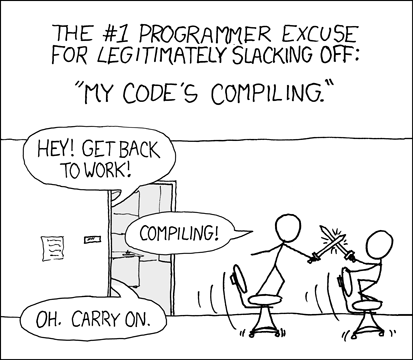
\includegraphics{compiling.png} \\
    \footnotesize\sffamily%
    Tiré de \href{http://xkcd.com/303/}{XKCD.com}
  \end{minipage}
\end{vplace}

\mainmatter

%%% Copyright (C) 2017 Vincent Goulet
%%%
%%% Ce fichier fait partie du projet «Programmer avec R»
%%% http://github.com/vigou3/programmer-avec-r
%%%
%%% Cette création est mise à disposition selon le contrat
%%% Attribution-Partage dans les mêmes conditions 4.0
%%% International de Creative Commons.
%%% http://creativecommons.org/licenses/by-sa/4.0/

\chapter{Éléments d'informatique pour programmeurs}
\label{chap:informatique}

Intro du chapitre

\section{Bref historique des langages de programmation}
\label{sec:informatique:historique}

Ada Lovelace (1815--1852) est généralement reconnue comme la première
auteure d'un algorithme et de ce que l'on appelle aujourd'hui un
programme informatique. C'est en son honneur qu'été nommé le langage
Ada conçu en réponse à un cahier de charges du département de la
Défense des États-Unis au début des années 1980.

Franchissons d'un bond les premiers jours de l'informatique et de la
programmation pour arriver aux ordinateurs électriques modernes, dans
les années 1940. On programme alors généralement ceux-ci en
\emph{assembleur}, un langage de très bas niveau facilement
interprétable par la machine, mais difficile à lire par des humains,
comme l'extrait de programme de la
\autoref{fig:informatique:assembleur} le démontre bien.

\begin{figure}
  \centering
  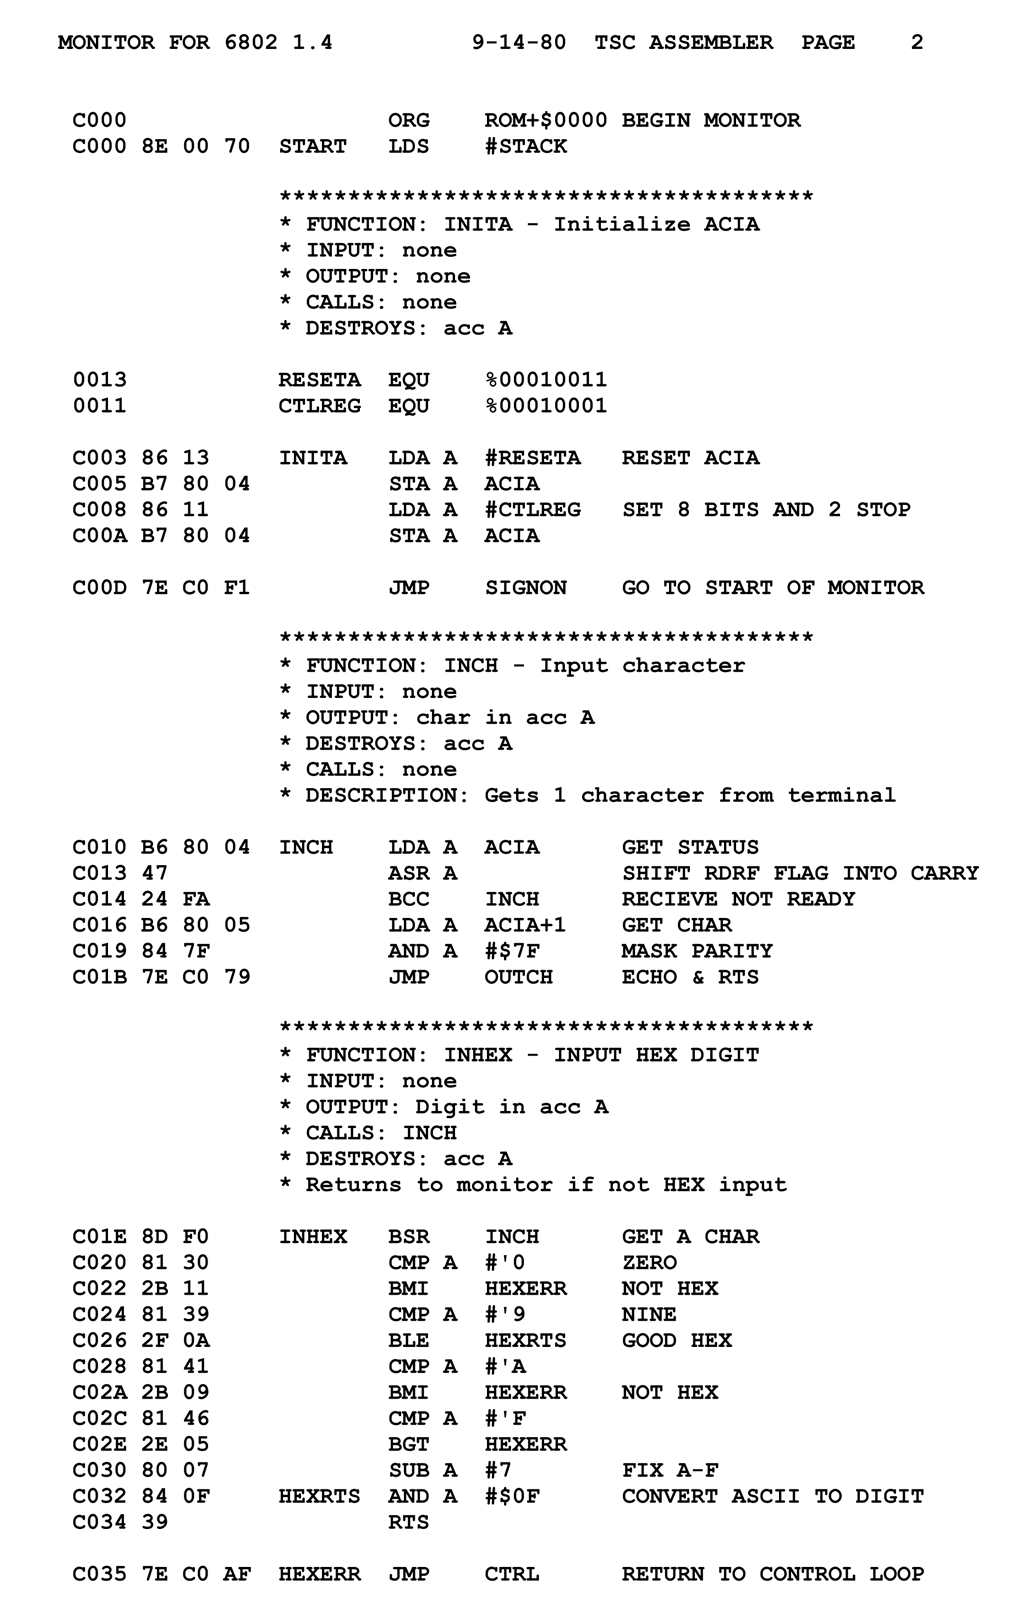
\includegraphics[trim=0 475 0 0, clip=true]{Motorola_6800_Assembly_Language.png}
  \caption[Programme en assembleur pour un microprocesseur 8~bits
  Motorola 6800.]{Extrait d'un programme en assembleur pour un
    microprocesseur 8~bits Motorola 6800. {\small Source:
      \link{https://commons.wikimedia.org/wiki/File\%3AMotorola_6800_Assembly_Language.png}{Wikimedia
        Commons}}}
  \label{fig:informatique:assembleur}
\end{figure}

Les premiers langages créés pour transmettre des instructions à un
ordinateur apparaissent dans les années 1950. Ils sont à l'origine
intimement liés à l'architecture d'un ordinateur: à chaque type
d'ordinateur son langage de programmation. Certaines contraintes ---
ou exigences --- des langages de l'époque proviennent aussi du support
physique alors utilisé pour stocker les programmes: les cartes
perforées.

\subsection{Fortran}
\label{sec:informatique:historique:fortran}

En 1954, l'ingénieur de IBM John Backus publie les spécifications du
langage FORTRAN (\emph{FORmula TRANslating System}). Le premier
compilateur voit le jour deux ans plus tard. Fortran (avec des
minuscules à partir de 1977) deviendra rapidement le langage standard
dans le calcul scientifique.

Plus d'un demi-siècle plus tard, l'empreinte de Fortran demeure
importante, notamment grâce aux bibliothèques d'algèbre linéaire
BLAS\footnote{%
  \emph{Basic Linear Algebra Subprograms};
  \link{http://www.netlib.org/blas}{}.} %
et LAPACK\footnote{%
  \emph{Linear Algebra PACKage};
  \link{http://www.netlib.org/lapack}{}.} %
auxquelles ont recours la plupart des progiciels scientifiques, dont
R. Le langage est toujours utilisé en calcul haute performance et pour
mesurer le rendement des superordinateurs.

\begin{figure}[t]
  \notebox{Dans le très recommandable film Les figures de l'ombre
    (\emph{Hidden Figures}, 2016), une des héroïnes entreprend de
    s'attaquer à la programmation des nouveaux ordinateurs de la NASA.
    On peut alors voir qu'elle apprend le Fortran.}
\end{figure}

\subsection{Lisp}
\label{sec:informatique:historique:lisp}

Le deuxième langage le plus ancien toujours largement diffusé est Lisp
(\emph{LISt Processing}). Créé par John McCarthy en 1958 en tant que
modèle pratique pour représenter des programmes, le Lisp est devenu le
langage de choix pour la recherche et les applications en intelligence
artificielle. Le terme Lisp désigne aujourd'hui une famille de
langages comprenant de nombreux dialectes, dont Common Lisp, Scheme et
Emacs Lisp.

Le Lisp se distingue en outre par une syntaxe simple en notation
préfixée (voir encadré), le support pour la programmation
fonctionnelle (\autoref{sec:informatique:paradigmes}) et la faculté de
manipuler le code source en tant que structure de données. Autre trait
distinctif: la syntaxe du Lisp fait un usage immodéré des parenthèses.

Le Lisp est entouré d'une aura de beauté et d'élégance dont peu
d'autres langages peuvent se targuer. Citons Eric Raymond dans
\link{http://www.catb.org/esr/faqs/hacker-howto.html}{\emph{How to
    Become a Hacker}}:
\begin{quote}
  Il faut apprendre le Lisp pour l'extraordinaire expérience d'éveil
  [\emph{enlightenment experience}] que procure le fait de finalement
  le comprendre; cette expérience fera de vous un meilleur programmeur
  pour toujours, même si vous n'avez plus vraiment à utiliser le Lisp.
\end{quote}

Pour illustrer encore davantage la place toute particulière qu'occupe
le Lisp en programmation, mentionnons également l'aphorisme selon
lequel «ceux qui ne connaissent pas le Lisp sont condamnés à le
réinventer», d'une certaine façon la version courte de la célèbre
\link{https://en.wikipedia.org/wiki/Greenspun\%27s_tenth_rule}{\emph{Greenspun's
    tenth rule of programming}}: %
\begin{quote}
  Tout programme en C ou en Fortran suffisamment complexe contient une
  implémentation mal spécifiée, pleine de bogues et lente de la moitié
  de Common Lisp.
\end{quote}
(Fait amusant à noter: il n'y a pas d'autres lois que la dixième, de
l'\link{http://philip.greenspun.com/bboard/q-and-a-fetch-msg?msg_id=000tgU}{aveu
  même de l'auteur}.)

\begin{figure}[t]
  \label{fig:informatique:notations}
  \setlength{\FrameRule}{1pt}
  \lstset{backgroundcolor=\color{codebg},
    frame=lr, rulecolor=\color{codebg},
    xleftmargin=3.4pt, xrightmargin=3.4pt}
  \begin{emphbox}{\mdseries Notations infixée, préfixée et suffixée}
    Les notations infixée (\emph{infix}), préfixée (\emph{prefix}) et
    suffixée (\emph{postfix}) sont trois manières différentes, mais
    équivalentes, d'écrire des expressions en mathématiques ou en
    programmation.

    Par exemple, l'opération d'addition de deux opérandes $x$ et $y$
    s'écrit en notation infixée
\begin{lstlisting}
x + y
\end{lstlisting}
    En notation préfixée, aussi appelée notation polonaise,
    l'opérateur est placé \emph{avant} les opérandes:
\begin{lstlisting}
+ x y
\end{lstlisting}
    On l'aura compris, en notation suffixée, ou notation polonaise
    inversée, l'opérateur apparait \emph{après} les opérandes:
\begin{lstlisting}
x y +
\end{lstlisting}
    Nous sommes davantage habitués à lire la notation infixée, quoique
    la notation préfixée nous soit familière pour les opérateurs à un
    seul opérande (comme la négation) ou pour les appels de fonctions.
    La notation suffixée n'a jamais recours aux parenthèses.

    La compagnie HP commercialise de très prisées calculatrices
    scientifiques utilisant la notation suffixée (libellées RPN pour
    \emph{Reverse Polish Notation}) depuis 1972.
  \end{emphbox}
\end{figure}

\subsection{COBOL}
\label{sec:informatique:historique:cobol}

Le troisième langage développé dans les années 1950 et toujours en
usage de nos jours est COBOL (\emph{COmmon Business Oriented
  Language}). Ce langage spécialisé dans les applications de gestion a
été créé en 1959 par un comité formé pour proposer un langage commun
pour l'administration américaine.

Le COBOL reste très utilisé dans de grandes entreprises, notamment
dans les institutions financières. La légende urbaine veut d'ailleurs
que les programmeurs COBOL soient comparativement très bien rémunérés
aujourd'hui sous l'effet combiné de leur rareté et de l'importance
opérationnelle des applications qu'ils doivent maintenir.

\subsection{Algol}
\label{sec:informatique:historique:algol}

Dès la fin de la décennie 1950, un comité de scientifiques se réunit à
Zurich pour concevoir ce que l'on voudrait voir devenir le langage de
programmation standard. De ces rencontres naîtra Algol
(\emph{ALGorithmic Oriented Language}) en 1958. Comme la plupart des
tentatives de définition d'un standard, c'est un échec: le langage est
populaire dans les milieux académiques, mais restera peu utilisé dans
les applications commerciales.

Cela dit, on doit à Algol plusieurs innovations importantes, de telle
sorte qu'un grand nombre des langages qui verront le jour par la suite
seront considérés comme ses descendants; le poster
\link{http://www.oreilly.com/go/languageposter}{\emph{History of
    Programming Languages}} de O'Reilly Media illustre ce fait à
merveille. \citet{Hoare:1973} a d'ailleurs cette jolie formule:
\begin{quote}
  Voici un langage très en avance sur son temps, il n'a pas seulement
  été une amélioration de ses prédécesseurs mais aussi une
  amélioration de presque tous ses successeurs.
\end{quote}


\begin{figure}[t]
  \centering
  \begin{minipage}{0.9\linewidth}
    \setkeys{Gin}{width=\textwidth}
    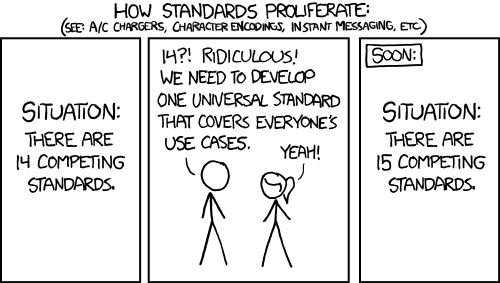
\includegraphics{standards} \\
    \footnotesize\sffamily%
    Tiré de \href{http://xkcd.com/927/}{XKCD.com}
  \end{minipage}
\end{figure}

\subsection{APL}
\label{sec:informatique:historique:apl}

Notre historique ne serait pas complet sans un mot sur APL (\emph{A
  Programming Language}, qui l'aurait cru). Même s'il n'a jamais connu
une diffusion importante, ce langage conçu par Kenneth Iverson autour
de 1962 n'en a pas moins eu une influence considérable sur la manière
de penser et de représenter les opérations mathématiques sur les
tableaux à plusieurs dimensions.

Doté d'une large gamme de symboles pour représenter des opérations et
d'une syntaxe tout à fait particulière --- les expressions sont
exécutées de droite à gauche! --- l'APL est remarquablement concis et
puissant; voir la \autoref{fig:informatique:apl} pour un aperçu. Le
revers de la cette médaille et ce qui a assurément nui à son adoption
à large échelle, c'est la difficulté que l'on éprouve à relire le
code. Assez pour que d'aucuns qualifient l'APL de «langage à écriture
seulement».

APL a pendant longtemps été un langage très prisé par les actuaires,
aussi subsiste-t-il du code dans certaines compagnies d'assurance. Le
modèle de traitement des vecteurs, matrices et tableaux de l'APL a
servi d'inspiration pour la conception du langage S --- nous y
reviendrons au \autoref{chap:presentation}.

Le langage continue sa vie aujourd'hui principalemnt sous forme de son
successeur, J.

\begin{figure}
  \centering
  \scalebox{0.4}{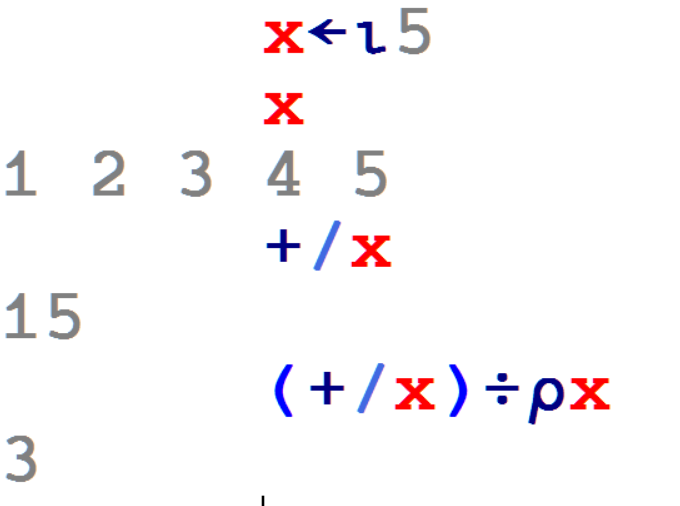
\includegraphics{APL_intro}}
  \caption[Opérations simples en APL.]{Opérations simples en APL. De
    haut en bas: génération des nombres de $1$ à $5$ et stockage dans
    la variable \code{x}; affichage du contenu de \code{x}; somme des
    éléments de \code{x}; moyenne des éléments de \code{x}. {\small Source:
    François-Dominique,
    \link{https://commons.wikimedia.org/w/index.php?curid=43207460}{Wikimedia
      Commons}, CC BY-SA 4.0}}
  \label{fig:informatique:apl}
\end{figure}

\subsection{C}
\label{sec:informatique:historique:c}

Le langage C a été inventé en 1972 chez Bell Labs par Ken Thompson et
Dennis Ritchie afin de réécrire le système d'exploitation UNIX
(\autoref{sec:informatique:os:unix}). Il demeure beaucoup utilisé pour
la programmation système: le noyau de systèmes d'exploitation comme
Windows et Linux sont développés en grande partie en C.

Le C est un langage de programmation généraliste considéré, selon les
standards actuels, comme de bas niveau. Pour illustrer, l'utilisateur
doit programmer des traitements comme la libération de la mémoire, la
vérification de la validité des indices sur les tableaux, l'ouverture
et la fermeture des fichiers, etc.

Le langage demeure l'un des plus utilisés dans le monde et son
influence est considérable. De nombreux langages plus modernes comme
\Cpp, C\# et Java reprennent des aspects de C. Le C est également
beaucoup utilisé pour le calcul numérique intensif, où il s'est en
quelque sorte substitué à Fortran. La plupart des progiciels
scientifiques --- dont R, encore une fois --- offrent la possibilité
d'appeler du code C lorsque la rapidité de calcul devient un enjeu. Le
gain en temps d'exécution doit toutefois être suffisamment grand pour
compenser le temps de développement plus long qu'exige le C par
rapport à des langages de plus haut niveau.

\begin{figure}[t]
  \notebox{Dans l'ouvrage désormais classique de \cite{KandR:1978}, le
    premier exemple d'un programme C affiche le message «\emph{hello,
      world}» à l'écran. Ça deviendra ensuite une tradition de
    démontrer le fonctionnement ou la syntaxe d'un langage avec cet
    exemple.}
\end{figure}

\subsection{Autres jalons}
\label{sec:informatique:historique:autres}

Nous nous sommes attardés jusqu'ici à des langages de programmation
vieux de plus de 40 ans à cause de leur importance historique et parce
qu'ils sont toujours utilisés couramment. De nombreux autres langages
ont vu le jour depuis, si bien qu'ils se comptent aujourd'hui par
milliers. En voici quelques autres ayant occupé une place
prépondérante dans l'histoire.

\begin{itemize}
\item Comme son nom l'indique, \textbf{\Cpp} (Bjarne Stroustrup, 1980)
  est un dérivé du C qui lui ajoute, en autres choses, la
  programmation orientée objet. Certains considèrent que {\Cpp}
  devrait être le point d'entrée de toute personne voulant débuter à
  programmer avec des langages de la famille du C. Le code C est
  compatible avec le \Cpp.
\item Principal représentant de l'ère Internet des années 1990,
  \textbf{Java} (James Gosling, 1995) a été conçu pour que le code
  écrit dans ce langage puisse s'exécuter sur n'importe quelle
  plateforme informatique sans nécessiter une nouvelle compilation. Il
  est donc très populaire dans les applications web ou embarquées. Sa
  syntaxe est fortement inspirée du \Cpp.
\item \textbf{Visual Basic} (Microsoft, 1991) permet de développer des
  applications de manière interactive en disposant des composantes sur
  un canevas. Le langage est aujourd'hui discontinué, mais son dérivé
  \textbf{Visual Basic for Applications} (VBA) demeure beaucoup
  utilisé dans les applications de la suite bureautique Office.
\item \textbf{Python} (Guido van Rossum, 1991) est un langage de haut
  niveau, orienté objet, multiplateforme et sous licence libre. C'est
  un des langages les plus utilisés aujourd'hui pour le calcul
  scientifique et l'analyse de données massives.
\end{itemize}

Certains langages de programmation ont une vocation généraliste,
certains visent des niches particulières, alors que d'autres cherchent
surtout à faire progresser l'état des connaissances dans la théorie
des langages. Quoi qu'il en soit, un langage de programmation demeure
un outil et, en informatique comme dans d'autres domaines, il convient
de choisir le meilleur outil pour accomplir une tâche donnée.

Nous invitons les lecteurs intéressés à en savoir davantage sur
l'histoire des langages de programmation en général, ou sur l'un ou
l'autre des langages mentionnés ci-dessus en particulier, à débuter
par les très complètes entrées de Wikipedia en
\link{https://fr.wikipedia.org/wiki/Histoire_des_langages_de_programmation}{français}
et en
\link{https://en.wikipedia.org/wiki/History_of_programming_languages}{anglais}.


\section{Sémantique et syntaxe}
\label{sec:informatique:semantique}

Il y a plusieurs parallèles à dresser entre les langages de
programmation et les langues parlées ou écrites: leur apprentissage
requiert de la pratique; on en connait jamais un trop grand nombre; le
premier est plus difficile à apprendre que les suivants.
L'informatique a également emprunté à la linguistique les notions de
\emph{sémantique} et de \emph{syntaxe}.

La sémantique est l'étude de ce que signifie un message ou un
programme informatique, c'est-à-dire de ce qu'il transmet ou exécute.
La syntaxe, quant à elle, étudie la structure du message ou du
programme. En simplifiant, disons que, pour une langue donnée, un
dictionnaire permet de connaître la sémantique, alors qu'une grammaire
décrit la syntaxe \citep{Hebenstreit:semantique}.

Par exemple, exprimons le message «J'ai soif» en anglais. Dire
«\emph{I am hungry}» relèverait d'une erreur de sémantique, puisque la
signification du message s'en trouve changée. En revanche, avec
«\emph{I have thirsty}» le bon message se rendra, mais peut-être pas
sans que l'erreur de syntaxe n'ait d'abord suscité une hésitation chez
l'interlocuteur.

Comme pour une langue, la maîtrise d'un langage de programmation exige
de respecter à la fois les règles de sémantique et les régles de
syntaxe du langage. Le second volet est relativement facile: si le
programme compile ou s'exécute, c'est généralement que la syntaxe est
respectée. Le respect de la sémantique, ou de la manière propre d'un
langage d'exprimer des idées, demande plus d'efforts et de pratique.


\section{Paradigmes de programmation}
\label{sec:informatique:paradigmes}

\section{Systèmes d'exploitation}
\label{sec:informatique:os}



%%% Local Variables:
%%% mode: latex
%%% TeX-engine: xetex
%%% TeX-master: "programmer-avec-r"
%%% End:

\chapter{Pr�sentation du langage S}
\label{presentation}


\section{Le langage S}
\label{presentation:langage}

Le S est un langage pour �programmer avec des donn�es� d�velopp� chez
Bell Laboratories (anciennement propri�t� de AT\&T, maintenant de
Lucent Technologies).

\begin{itemize}
\item Ce n'est pas seulement un �autre� environnement statistique
  (comme SPSS ou SAS, par exemple), mais bien un langage de
  programmation complet et autonome.
\item Inspir� de plusieurs langages, dont l'APL et le Lisp, le S est:
  \begin{itemize}
  \item interpr�t� (et non compil�);
  \item sans d�claration obligatoire des variables;
  \item bas� sur la notion de vecteur;
  \item particuli�rement puissant pour les applications math�matiques
    et statistiques (et donc actuarielles).
  \end{itemize}
\end{itemize}


\section{Les moteurs S}
\label{presentation:moteurs}

Il existe quelques �moteurs� ou dialectes du langage S.

\begin{itemize}
\item Le plus connu est S-Plus, un logiciel commercial de
  Insightful Corporation (Bell Labs octroie � Insightful la licence
  exclusive de son syst�me S).
\item \textsf{R}, ou GNU S, est une version libre (\emph{Open Source})
  �\emph{not unlike S}�.
\end{itemize}

S-Plus et \textsf{R} constituent tous deux des environnements int�gr�s
de manipulation de donn�es, de calcul et de pr�paration de graphiques.


\section{O� trouver de la documentation}
\label{presentation:doc}

S-Plus est livr� avec quatre livres (disponibles en format PDF depuis
le menu \texttt{Help} de l'interface graphique), mais aucun ne s'av�re
vraiment utile pour apprendre le langage S.

Plusieurs livres --- en versions papier ou �lectronique, gratuits ou
non --- ont �t� publi�s sur S-Plus et \textsf{R}. On trouvera des
listes exhaustives dans les sites de Insightful et du projet
\textsf{R}:
\begin{itemize}
\item \url{http://www.insightful.com/support/splusbooks.asp}
\item \url{http://www.r-project.org} (dans la section
  \texttt{Documentation}).
\end{itemize}

De plus, les ouvrages de \citet{Sprogramming,MASS} constituent des
r�f�rences sur le langage S devenues au cours des derni�res ann�es des
standards \emph{de facto}.


\section{Interfaces pour S-Plus et \textsf{R}}
\label{presentation:interfaces}

Provenant du monde Unix, tant S-Plus que \textsf{R} sont d'abord et
avant tout des applications en ligne de commande (\texttt{sqpe.exe} et
\texttt{rterm.exe} sous Windows).

\begin{itemize}
\item S-Plus poss�de toutefois une interface graphique �labor�e
  permettant d'utiliser le logiciel sans trop conna�tre le langage de
  programmation.
\item \textsf{R} dispose �galement d'une interface graphique
  rudimentaire sous Windows et Mac OS.
\item L'�dition s�rieuse de code S b�n�ficie cependant grandement d'un
  bon �diteur de texte.
\item � la question 6.2 de la foire aux questions (FAQ) de \textsf{R},
  �Devrais-je utiliser \textsf{R} � l'int�rieur de
  Emacs?�\index{Emacs}, la r�ponse est: �Oui, absolument.� Nous
  partageons cet avis, aussi ce document supposera-t-il que S-Plus ou
  \textsf{R} sont utilis�s � l'int�rieur de GNU Emacs avec le mode
  ESS\index{ESS}.
\item Autre option: WinEdt (partagiciel) avec l'ajout R-WinEdt.
\end{itemize}


\section{Installation de Emacs avec ESS}
\label{presentation:emacs}

Il n'existe pas de proc�dure d'installation similaire aux autres
applications Windows pour Emacs.  L'installation n'en demeure pas
moins tr�s simple: il suffit de d�compresser un ensemble de fichiers
au bon endroit.

\begin{itemize}
\item Pour une installation simplifi�e de Emacs et ESS, consulter le
  site Internet
  \begin{quote}
    \url{http://vgoulet.act.ulaval.ca/pub/emacs/}
  \end{quote}
  On y trouve une version modifi�e de GNU Emacs et des instructions
  d'installation d�taill�es.
\item L'annexe \ref{ess} pr�sente les plus importantes commandes �
  conna�tre pour utiliser Emacs et le mode ESS.
\end{itemize}


\section{D�marrer et quitter S-Plus ou \textsf{R}}
\label{presentation:demarrer}

On suppose ici que S-Plus ou R sont utilis�s � l'int�rieur de Emacs.

\begin{itemize}
\item Pour d�marrer \textsf{R} \R � l'int�rieur de Emacs:
\begin{verbatim}
M-x R RET
\end{verbatim}
  puis sp�cifier un dossier de travail (voir la section
  \ref{presentation:workspace}). Une console \textsf{R} est ouverte
  dans une fen�tre (\emph{buffer} dans la terminologie de Emacs)
  nomm�e \texttt{*R*}.
\item Pour d�marrer S-Plus sous Windows, \Splus la proc�dure est
  similaire, sauf que la commande � utiliser est
\begin{verbatim}
M-x Sqpe RET
\end{verbatim}
  Consulter l'annexe \ref{s-plus_windows} pour de plus amples
  d�tails.
\item Pour quitter, deux options sont disponibles:
  \begin{enumerate}
  \item Taper \fonction{q()} � la ligne de commande.
  \item Dans Emacs, faire \ess{C-c C-q}. ESS va alors s'occuper de
    fermer le processus S ainsi que tous les \emph{buffers} associ�s �
    ce processus.
  \end{enumerate}
\end{itemize}


\section{Strat�gies de travail}
\label{presentation:strategies}

Il existe principalement deux fa�ons de travailler avec S-Plus et
\textsf{R}.
\begin{enumerate}
\item Le code est virtuel et les objets sont r�els. C'est l'approche
  qu'encouragent les interfaces graphiques, mais c'est aussi la moins
  pratique � long terme. On entre des expressions directement � la
  ligne de commande pour les �valuer imm�diatement.
\begin{Schunk}
\begin{Sinput}
> 2 + 3
\end{Sinput}
\begin{Soutput}
[1] 5
\end{Soutput}
\begin{Sinput}
> -2 * 7
\end{Sinput}
\begin{Soutput}
[1] -14
\end{Soutput}
\begin{Sinput}
> exp(1)
\end{Sinput}
\begin{Soutput}
[1] 2.718282
\end{Soutput}
\begin{Sinput}
> log(exp(1))
\end{Sinput}
\begin{Soutput}
[1] 1
\end{Soutput}
\end{Schunk}
  Les objets cr��s au cours d'une session de travail sont sauvegard�s.
  Par contre, � moins d'avoir �t� sauvegard� dans un fichier, le code
  utilis� pour cr�er ces objets est perdu lorsque l'on quitte S-Plus
  ou \textsf{R}.
\item Le code est r�el et les objets sont virtuels. C'est l'approche
  que nous favorisons. Le travail se fait essentiellement dans des
  fichiers de script (de simples fichiers de texte) dans lesquels sont
  sauvegard�es les expressions (parfois complexes!) et le code des
  fonctions personnelles. Les objets sont cr��s au besoin en ex�cutant
  le code. Emacs permet ici de passer efficacement des fichiers de
  script � l'ex�cution du code:
  \begin{enumerate}[i)]
  \item d�marrer un processus S-Plus (\texttt{M-x Sqpe}) ou
    \textsf{R} (\texttt{M-x R}) et sp�cifier le dossier de travail;
  \item ouvrir un fichier de script avec \ess{C-x C-f}. Pour cr�er un
    nouveau fichier, ouvrir un fichier inexistant;
  \item positionner le curseur sur une expression et faire \ess{C-c
      C-n} pour l'�valuer;
  \item le r�sultat appara�t dans le \emph{buffer} \texttt{*S+6*} ou
    \texttt{*R*}.
  \end{enumerate}
\end{enumerate}


\section{Gestion des projets ou environnements de travail}
\label{presentation:workspace}

S-Plus et \textsf{R} ont une mani�re diff�rente mais tout aussi
particuli�re de sauvegarder les objets cr��s au cours d'une session de
travail.
\begin{itemize}
\item Tous deux doivent travailler dans un dossier et non avec des
  fichiers individuels.
\item Dans S-Plus, \Splus tout objet cr�� au cours d'une session de
  travail est sauvegard� de fa�on permanente sur le disque dur dans le
  sous-dossier \texttt{\_\_Data} du dossier de travail.
\item Dans \textsf{R}, \R les objets cr��s sont conserv�s en m�moire
  jusqu'� ce que l'on quitte l'application ou que l'on enregistre le
  travail avec la commande \fonction{save.image()}. L'environnement de
  travail (\emph{workspace}) est alors sauvegard� dans le fichier
  \texttt{.RData} du dossier de travail.
\end{itemize}

Le dossier de travail est d�termin� au lancement de l'application.
\begin{itemize}
\item Avec Emacs et ESS, on doit sp�cifier le dossier de travail
  chaque fois que l'on d�marre un processus S-Plus ou R.
\item Les interfaces graphiques permettent �galement de sp�cifier le
  dossier de travail.
  \begin{itemize}
    \sloppy
  \item Dans \Splus l'interface graphique de S-Plus, choisir
    \texttt{General Settings} dans le menu \texttt{Options}, puis
    l'onglet \texttt{Startup}. Cocher la case \texttt{Prompt for
      project folder}.  Consulter �galement le chapitre 13 du guide de
    l'utilisateur de S-Plus.
  \item Dans \R l'interface graphique de \textsf{R}, le plus simple
    consiste � changer le dossier de travail � partir du menu
    \texttt{Fichier|Changer le r�pertoire courant...} Consulter aussi
    la \emph{R for Windows FAQ}.
  \end{itemize}
\end{itemize}


\section{Consulter l'aide en ligne}
\label{presentation:aide}

Les rubriques d'aide des diverses fonctions disponibles dans S-Plus et
\textsf{R} contiennent une foule d'informations ainsi que des exemples
d'utilisation. Leur consultation est tout � fait essentielle.

\begin{itemize}
\item Pour consulter la rubrique d'aide de la fonction \code{foo},
  on peut entrer � la ligne de commande
\begin{Schunk}
\begin{Sinput}
> ?foo
\end{Sinput}
\end{Schunk}
\item Dans Emacs, \code{C-c C-v foo RET}\indexess{C-c C-v} ouvrira la
  rubrique d'aide de la fonction \code{foo} dans un nouveau
  \emph{buffer}.
\item Plusieurs touches de raccourcis facilitent la consultation des
  rubriques d'aide (voir la carte de r�f�rence ESS).
\item Entre autres, la touche \texttt{l} permet d'ex�cuter ligne par
  ligne les exemples se trouvant � la fin de chaque rubrique d'aide.
\end{itemize}


\section{Exemples}
\label{presentation:exemples}

\lstinputlisting{presentation.R}


\section{Exercices}
\label{presentation:exercices}

\begin{exercice}
  D�marrer un processus S-Plus ou \textsf{R} � l'int�rieur de Emacs.
\end{exercice}

\begin{exercice}
  Ex�cuter un � un les exemples de la section pr�c�dente. Une version
  �lectronique du code de cette section est disponible dans le site
  mentionn� dans la pr�face.
\end{exercice}

\begin{exercice}
  Consulter les rubriques d'aide d'une ou plusieurs des fonctions
  rencontr�es lors de l'exercice pr�c�dent. Observer d'abord comment
  les ru\-bri\-ques d'aide sont structur�es --- elles sont toutes
  identiques --- puis ex�cuter quelques lignes d'exemples.
\end{exercice}

\begin{exercice}
  Lire le chapitre 1 de \cite{MASS} et ex�cuter les commandes de
  l'exemple de session de travail de la section 1.3. Bien que
  davantage orient� vers les application statistiques que vers la
  programmation, cet exemple d�montre quelques-unes des possibilit�s
  du langage S.
\end{exercice}

%%% Local Variables:
%%% mode: latex
%%% TeX-master: "introduction_programmation_S"
%%% End:

\chapter{Bases du langage S}
\label{bases}


Ce chapitre pr�sente les bases du langage S, soit les notions
d'expression et d'affectation, la description d'un objet S et les
mani�res de cr�er les objets les plus usuels lorsque le S est utilis�
comme langage de programmation.

\section{Commandes S}
\label{bases:commandes}

Toute commande S est soit une \emph{expression}\index{expression},
soit une \emph{affectation}\index{affectation}.
\begin{itemize}
\item Normalement, une expression est imm�diatement �valu�e et le
  r�sultat est affich� � l'�cran:
\begin{Schunk}
\begin{Sinput}
> 2 + 3
\end{Sinput}
\begin{Soutput}
[1] 5
\end{Soutput}
\begin{Sinput}
> pi
\end{Sinput}
\begin{Soutput}
[1] 3.141593
\end{Soutput}
\begin{Sinput}
> cos(pi/4)
\end{Sinput}
\begin{Soutput}
[1] 0.7071068
\end{Soutput}
\end{Schunk}
\item Lors d'une affectation, une expression est �valu�e, mais le
  r�sultat est stock� dans un objet (variable) et rien n'est affich� �
  l'�cran. Le symbole d'affectation est \Fonction{<-} (ou
  \Fonction{->}).
\begin{Schunk}
\begin{Sinput}
> a <- 5
> a
\end{Sinput}
\begin{Soutput}
[1] 5
\end{Soutput}
\begin{Sinput}
> b <- a
> b
\end{Sinput}
\begin{Soutput}
[1] 5
\end{Soutput}
\end{Schunk}
\item �viter d'utiliser l'op�rateur \fonction{=} pour affecter une
  valeur � une variable, puisqu'il ne fonctionne que dans certaines
  situations seulement.
\item Dans S-Plus (mais plus dans \textsf{R} depuis la version 1.8.0),
  on peut �galement affecter avec le caract�re �\fonction{\_}�, mais cet
  emploi est fortement d�courag� puisqu'il rend le code difficile �
  lire. Dans le mode ESS de Emacs, taper ce caract�re g�n�re carr�ment
  \verb*| <- |.
\end{itemize}

\begin{astuce}
  Il arrive fr�quemment que l'on souhaite affecter le r�sultat d'un
  calcul dans un objet et en m�me temps voir ce r�sultat. Pour ce
  faire, placer l'affectation entre parenth�ses (l'op�ration
  d'affectation devient alors une nouvelle expression):
\begin{Schunk}
\begin{Sinput}
> (a <- 2 + 3)
\end{Sinput}
\begin{Soutput}
[1] 5
\end{Soutput}
\end{Schunk}
\end{astuce}


\section{Conventions pour les noms d'objets}
\index{noms d'objets!conventions}
\label{bases:noms}

Les caract�res permis pour les noms d'objets sont les lettres a--z,
A--Z, les chiffres 0--9 et le point �.�. Le caract�re \R �\code{\_}�
est maintenant permis dans \textsf{R}, mais son utilisation est
d�courag�e.

\begin{itemize}
\item Les noms d'objets ne peuvent commencer par un chiffre.
\item Le S est sensible � la casse, ce qui signifie que \code{foo},
  \code{Foo} et \code{FOO} sont trois objets distincts. Un moyen
  simple d'�viter des erreurs li�es � la casse consiste � n'employer
  que des lettres minuscules.
\item Certains noms sont utilis�s par le syst�me, aussi vaut-il mieux
  �viter de les utiliser. En particulier, �viter d'utiliser
  \begin{center}
    \code{c}, \code{q}, \code{t}, \code{C}, \code{D},
    \code{I}, \code{diff}, \code{length}, \code{mean},
    \code{pi}, \code{range}, \code{var}.
  \end{center}
\item \index{noms d'objets!r�serv�s} Certains mots sont r�serv�s pour
  le syst�me et il est interdit de les utiliser comme nom d'objet. Les
  mots r�serv�s sont:
  \begin{center}
    \code{Inf}, \code{NA}, \code{NaN},
    \code{NULL} \\
    \code{break}, \code{else},
    \code{for}, \code{function}, \code{if}, \code{in},
    \code{next}, \code{repeat}, \code{return}, \code{while}.
  \end{center}
\item Dans S-Plus 6.1 et plus, \Splus
  \code{T}\index{T@\code{T}|see{\code{TRUE}}} et \objet{TRUE} (vrai),
  ainsi que \code{F}\index{F@\code{F}|see{\code{FALSE}}} et
  \objet{FALSE} (faux) sont �galement des noms r�serv�s.
\item Dans \textsf{R}, \R les noms \code{TRUE} et \code{FALSE}
  sont �galement r�serv�s. Les variables \code{T} et \code{F}
  prennent par d�faut les valeurs \code{TRUE} et \code{FALSE},
  respectivement, mais peuvent �tre r�affect�es.
\begin{Schunk}
\begin{Sinput}
> T
\end{Sinput}
\begin{Soutput}
[1] TRUE
\end{Soutput}
\end{Schunk}
\begin{Schunk}
\begin{Sinput}
> TRUE <- 3
\end{Sinput}
\end{Schunk}
\begin{Schunk}
\begin{Soutput}
Erreur dans TRUE <- 3 : membre gauche de
l'assignation (do_set) incorrect
\end{Soutput}
\end{Schunk}
\begin{Schunk}
\begin{Sinput}
> (T <- 3)
\end{Sinput}
\begin{Soutput}
[1] 3
\end{Soutput}
\end{Schunk}
\end{itemize}


\section{Les objets S}
\label{bases:objets}

Tout dans le langage S est un objet, m�me les fonctions et les
op�rateurs. Les objets poss�dent au minimum un \emph{mode} et une
\emph{longueur}.

\begin{itemize}
\item Le mode d'un objet est obtenu avec la fonction \Fonction{mode}.
\begin{Schunk}
\begin{Sinput}
> v <- c(1, 2, 5, 9)
> mode(v)
\end{Sinput}
\begin{Soutput}
[1] "numeric"
\end{Soutput}
\end{Schunk}
\item La longueur d'un objet est obtenue avec la fonction
  \Fonction{length}.
\begin{Schunk}
\begin{Sinput}
> length(v)
\end{Sinput}
\begin{Soutput}
[1] 4
\end{Soutput}
\end{Schunk}
\item Certains objets sont �galement dot�s d'un ou plusieurs
  \emph{attributs}.
\end{itemize}


\subsection{Modes et types de donn�es}

Le mode\Index{mode} prescrit ce qu'un objet peut contenir. � ce titre,
un objet ne peut avoir qu'un seul mode. Le tableau \ref{tab:modes}
contient la liste des modes disponibles en S. � chacun de ces modes
correspond une fonction du m�me nom servant � cr�er un objet de ce
mode.

\begin{table}
  \centering
  \begin{tabular}{ll}
    \toprule
    \Mode{numeric}   & nombres r�els \\
    \Mode{complex}   & nombres complexes \\
    \Mode{logical}   & valeurs bool�ennes (vrai/faux) \\
    \Mode{character} & cha�nes de caract�res \\
    \Mode{function}  & fonction \\
    \Mode{list}      & donn�es quelconques \\
    \bottomrule
  \end{tabular}
  \caption{Modes disponibles et contenus correspondants}
  \label{tab:modes}
\end{table}

\subsection{Longueur}

La longueur\Index{longueur} d'un objet est �gale au nombre d'�l�ments
qu'il contient.

\begin{itemize}
\item La longueur d'une cha�ne de caract�res est toujours 1. Un
  objet de mode \code{character} doit contenir plusieurs cha�nes
  de caract�res pour que sa longueur soit sup�rieure � 1.
\begin{Schunk}
\begin{Sinput}
> v <- "actuariat"
> length(v)
\end{Sinput}
\begin{Soutput}
[1] 1
\end{Soutput}
\begin{Sinput}
> v <- c("a", "c", "t", "u", "a", "r", "i", 
+     "a", "t")
> length(v)
\end{Sinput}
\begin{Soutput}
[1] 9
\end{Soutput}
\end{Schunk}
\item Un objet peut �tre de longueur 0 et doit alors �tre interpr�t�
  comme un contenant vide\index{vide|see{\code{NULL}}}.
\begin{Schunk}
\begin{Sinput}
> v <- numeric(0)
> length(v)
\end{Sinput}
\begin{Soutput}
[1] 0
\end{Soutput}
\end{Schunk}
\end{itemize}


\subsection{Attributs}

Les attributs\Index{attribut} d'un objet sont des �l�ments
d'information additionnels li�s � cet objet. La liste des attributs
les plus fr�quemment rencontr�s se trouve au tableau
\ref{tab:attributs}. Pour chaque attribut, il existe une fonction du
m�me nom servant � extraire l'attribut correspondant d'un objet.

\begin{table}
  \centering
  \begin{tabular}{ll}
    \toprule
    \Attribut{class}    &
    affecte le comportement d'un objet \\
    \Attribut{dim}      &
    dimensions\index{dimension} des matrices et tableaux \\
    \Attribut{dimnames} &
    �tiquettes\index{etiquette@�tiquette} des dimensions des matrices
    et tableaux \\
    \Attribut{names}    &
    �tiquettes des �l�ments d'un objet \\
    \bottomrule
  \end{tabular}
  \caption{Attributs les plus usuels d'un objet et leur effet}
  \label{tab:attributs}
\end{table}


\subsection{L'objet sp�cial \code{NA}}

\Objet{NA} est fr�quemment utilis� pour repr�senter les donn�es
manquantes.

\begin{itemize}
\item Son mode est \mode{logical}.
\item Toute op�ration impliquant une donn�e \code{NA} a comme
  r�sultat \code{NA}.
\item Certaines fonctions (\fonction{sum}, \fonction{mean}, par
  exemple) ont par cons�quent un argument \Argument{na.rm} qui,
  lorsque \code{TRUE}, �limine les donn�es manquantes avant de
  faire un calcul.
\item La fonction \Fonction{is.na} permet de tester si les �l�ments
  d'un objet sont \code{NA} ou non.
\end{itemize}

\subsection{L'objet sp�cial \code{NULL}}

\Objet{NULL} repr�sente �rien�, ou le vide.

\begin{itemize}
\item Son mode est \Mode{NULL}.
\item Sa longueur est 0.
\item Diff�rent d'un objet vide:
  \begin{itemize}
  \item un objet de longueur 0 est un contenant vide;
  \item \code{NULL} est �pas de contenant�.
  \end{itemize}
\item La fonction \Fonction{is.null} teste si un objet est \code{NULL}
  ou non.
\end{itemize}


\section{Vecteurs}
\label{bases:vecteurs}

En S, � peu de choses pr�s, \emph{tout} est un vecteur\index{vecteur}.
(Il n'y a pas de notion de scalaire.)

\begin{itemize}
\item Dans un vecteur simple, tous les �l�ments doivent �tre du
  m�me mode.
\item Il est possible (et souvent souhaitable) de donner une �tiquette
  � chacun des �l�ments d'un vecteur.
\begin{Schunk}
\begin{Sinput}
> (v <- c(a = 1, b = 2, c = 5))
\end{Sinput}
\begin{Soutput}
a b c 
1 2 5 
\end{Soutput}
\begin{Sinput}
> v <- c(1, 2, 5)
> names(v) <- c("a", "b", "c")
> v
\end{Sinput}
\begin{Soutput}
a b c 
1 2 5 
\end{Soutput}
\end{Schunk}
\item Les fonctions de base pour cr�er des vecteurs sont:
  \begin{itemize}
  \item \Fonction{c} (concat�nation);
  \item \Fonction{numeric} (vecteur de mode \mode{numeric});
  \item \Fonction{logical} (vecteur de mode \mode{logical});
  \item \Fonction{character} (vecteur de mode \mode{character}).
  \end{itemize}
\item L'indi�age dans un vecteur se fait avec \fonction{[\ ]}. On
  peut extraire un �l�ment d'un vecteur par sa position ou par son
  �tiquette, si elle existe (auquel cas cette approche est beaucoup
  plus s�re).
\begin{Schunk}
\begin{Sinput}
> v[3]
\end{Sinput}
\begin{Soutput}
c 
5 
\end{Soutput}
\begin{Sinput}
> v["c"]
\end{Sinput}
\begin{Soutput}
c 
5 
\end{Soutput}
\end{Schunk}
  La section \ref{bases:indicage} traite plus en d�tail de l'indi�age de
  vecteurs et matrices.
\end{itemize}


\section{Matrices et tableaux}
\label{bases:matrices}

Une matrice\index{matrice} ou, de fa�on plus g�n�rale, un
tableau\index{tableau} (\emph{array}) n'est rien d'autre qu'un vecteur
dot� d'un attribut \attribut{dim}. � l'interne, une matrice est donc
stock�e sous forme de vecteur.

\begin{itemize}
\item La fonction de base pour cr�er des matrices est
  \Fonction{matrix}.
\item La fonction de base pour cr�er des tableaux est
  \Fonction{array}.
\item \emph{Important}: \warning les matrices et tableaux sont remplis
  en faisant d'abord varier la premi�re dimension, puis la seconde,
  etc. Pour les matrices, cela revient � remplir par colonne.
\begin{Schunk}
\begin{Sinput}
> matrix(1:6, nrow = 2, ncol = 3)
\end{Sinput}
\begin{Soutput}
     [,1] [,2] [,3]
[1,]    1    3    5
[2,]    2    4    6
\end{Soutput}
\begin{Sinput}
> matrix(1:6, nrow = 2, ncol = 3, byrow = TRUE)
\end{Sinput}
\begin{Soutput}
     [,1] [,2] [,3]
[1,]    1    2    3
[2,]    4    5    6
\end{Soutput}
\end{Schunk}
\item L'indi�age \index{indi�age!matrice} d'une matrice se fait
  �galement avec \fonction{[\ ]}. On extrait les �l�ments en pr�cisant
  leurs positions sous la forme (ligne, colonne) dans la matrice, ou
  encore leurs positions dans le vecteur sous-jacent.
\begin{Schunk}
\begin{Sinput}
> (m <- matrix(c(40, 80, 45, 21, 55, 32), 
+     nrow = 2, ncol = 3))
\end{Sinput}
\begin{Soutput}
     [,1] [,2] [,3]
[1,]   40   45   55
[2,]   80   21   32
\end{Soutput}
\begin{Sinput}
> m[1, 2]
\end{Sinput}
\begin{Soutput}
[1] 45
\end{Soutput}
\begin{Sinput}
> m[3]
\end{Sinput}
\begin{Soutput}
[1] 45
\end{Soutput}
\end{Schunk}
\item La fonction \Fonction{rbind} permet de fusionner verticalement
  deux matrices (ou plus) ayant le m�me nombre de colonnes.
\begin{Schunk}
\begin{Sinput}
> n <- matrix(1:9, nrow = 3)
> rbind(m, n)
\end{Sinput}
\begin{Soutput}
     [,1] [,2] [,3]
[1,]   40   45   55
[2,]   80   21   32
[3,]    1    4    7
[4,]    2    5    8
[5,]    3    6    9
\end{Soutput}
\end{Schunk}
\item La fonction \Fonction{cbind} permet de fusionner horizontalement
  deux matrices (ou plus) ayant le m�me nombre de lignes.
\begin{Schunk}
\begin{Sinput}
> n <- matrix(1:4, nrow = 2)
> cbind(m, n)
\end{Sinput}
\begin{Soutput}
     [,1] [,2] [,3] [,4] [,5]
[1,]   40   45   55    1    3
[2,]   80   21   32    2    4
\end{Soutput}
\end{Schunk}
\end{itemize}


\section{Listes}
\label{bases:listes}

Une liste\index{liste} est un type de vecteur sp�cial dont les
�l�ments peuvent �tre de n'importe quel mode, y compris le mode
\mode{list} (ce qui permet d'embo�ter des listes).

\begin{itemize}
\item La fonction de base pour cr�er des listes est \Fonction{list}.
\item Il est g�n�ralement pr�f�rable de nommer les �l�ments d'une
  liste. Il est en effet plus simple et s�r d'extraire les �l�ments
  par leur �tiquette.
\item L'extraction\Index{indi�age!liste} des �l�ments d'une liste peut
  se faire de deux fa�ons:
  \begin{enumerate}
  \item avec des doubles crochets \fonction{[[\ ]]};
  \item par leur �tiquette avec \code{nom.liste\$etiquette.element}.
  \end{enumerate}
\item La fonction \Fonction{unlist} convertit une liste en un vecteur
  simple. Attention, cette fonction peut �tre destructrice si la
  structure de la liste est importante.
\end{itemize}


\section{\emph{Data frames}}
\label{bases:dataframes}

Les vecteurs, matrices, tableaux (\emph{arrays}) et listes sont les
types d'objets les plus fr�quemment utilis�s en S pour la
programmation de fonctions personnelles ou la simulation. L'analyse de
donn�es --- la r�gression lin�aire, par exemple --- repose toutefois
davantage sur les \emph{data frames}\Index{data frame}.

\begin{itemize}
\item Un \emph{data frame} est une liste de classe \classe{data.frame}
  dont tous les �l�ments sont de la m�me longueur.
\item G�n�ralement repr�sent� sous la forme d'un tableau � deux
  dimensions (visuellement similaire � une matrice). Chaque �l�ment de
  la liste sous-jacente correspond � une colonne.
\item On peut donc obtenir les �tiquettes des colonnes avec la fonction
  \fonction{names} (ou \fonction{colnames} \R dans \textsf{R}).  Les
  �tiquettes des lignes sont quant � elles obtenues avec
  \fonction{row.names} (ou \fonction{rownames} dans \textsf{R}).
\item Plus g�n�ral qu'une matrice puisque les colonnes peuvent �tre de
  modes diff�rents (\mode{numeric}, \mode{complex}, \mode{character}
  ou \mode{logical}).
\item Peut �tre indic� � la fois comme une liste et comme une matrice.
\item Cr�� avec la fonction \Fonction{data.frame} ou
  \Fonction{as.data.frame} (pour convertir une matrice en \emph{data
    frame}, par exemple).
\item Les fonctions \fonction{rbind} et \fonction{cbind} peuvent �tre
  utilis�es pour ajouter des lignes ou des colonnes, respectivement.
\item On peut rendre les colonnes d'un \emph{data frame} (ou d'une
  liste) visibles dans l'espace de travail avec la fonction
  \Fonction{attach}, puis les masquer avec \Fonction{detach}.
\end{itemize}

Ce type d'objet est moins important lors de l'apprentissage du langage
de programmation.




\section{Indi�age}
\label{bases:indicage}

L'indi�age des vecteurs\Index{indi�age!vecteur} et
matrices\Index{indi�age!matrice} a d�j� �t� bri�vement pr�sent� aux
sections \ref{bases:vecteurs} et \ref{bases:matrices}. La pr�sente
section contient plus de d�tails sur cette proc�dure des plus communes
lors de l'utilisation du langage S. On se concentre toutefois sur le
traitement des vecteurs. Se r�f�rer �galement � \citet[section
2.3]{MASS} pour de plus amples renseignements.

Il existe quatre fa�ons d'indicer un vecteur dans le langage S. Dans
tous les cas, l'indi�age se fait � l'int�rieur de crochets \Fonction{[\ ]}.
\begin{enumerate}
\item Avec un vecteur d'entiers positifs. Les �l�ments se trouvant aux
  positions correspondant aux entiers sont extraits du vecteur, dans
  l'ordre. C'est la technique la plus courante.
\begin{Schunk}
\begin{Sinput}
> letters[c(1:3, 22, 5)]
\end{Sinput}
\begin{Soutput}
[1] "a" "b" "c" "v" "e"
\end{Soutput}
\end{Schunk}
\item Avec un vecteur d'entiers n�gatifs. Les �l�ments se trouvant aux
  positions correspondant aux entiers n�gatifs sont alors
  \emph{�limin�s} du vecteur.
\begin{Schunk}
\begin{Sinput}
> letters[c(-(1:3), -5, -22)]
\end{Sinput}
\begin{Soutput}
 [1] "d" "f" "g" "h" "i" "j" "k" "l" "m" "n" "o" "p"
[13] "q" "r" "s" "t" "u" "w" "x" "y" "z"
\end{Soutput}
\end{Schunk}
\item Avec un vecteur bool�en. Le vecteur d'indi�age doit alors �tre
  de la m�me longueur que le vecteur indic�. Les �l�ments
  correspondant � une valeur \code{TRUE} sont extraits du vecteur,
  alors que ceux correspondant � \code{FALSE} sont �limin�s.
\begin{Schunk}
\begin{Sinput}
> letters > "f" & letters < "q"
\end{Sinput}
\begin{Soutput}
 [1] FALSE FALSE FALSE FALSE FALSE FALSE  TRUE  TRUE
 [9]  TRUE  TRUE  TRUE  TRUE  TRUE  TRUE  TRUE  TRUE
[17] FALSE FALSE FALSE FALSE FALSE FALSE FALSE FALSE
[25] FALSE FALSE
\end{Soutput}
\begin{Sinput}
> letters[letters > "f" & letters < "q"]
\end{Sinput}
\begin{Soutput}
 [1] "g" "h" "i" "j" "k" "l" "m" "n" "o" "p"
\end{Soutput}
\end{Schunk}
\item Avec une cha�ne de caract�res. Utile pour extraire les �l�ments
  d'un vecteur � condition que ceux-ci soient nomm�s.
\begin{Schunk}
\begin{Sinput}
> x <- c(Rouge = 2, Bleu = 4, Vert = 9, Jaune = -5)
> x[c("Bleu", "Jaune")]
\end{Sinput}
\begin{Soutput}
 Bleu Jaune 
    4    -5 
\end{Soutput}
\end{Schunk}
\end{enumerate}


\section{Exemples}
\label{bases:exemples}

\lstinputlisting{bases.R}


\section{Exercices}
\label{bases:exercices}

\Opensolutionfile{reponses}[reponses-bases]
\Writetofile{reponses}{\protect\section*{Chapitre \protect\ref{bases}}}

\begin{exercice}
  \begin{enumerate}
  \item �crire une expression S pour cr�er la liste suivante:
\begin{Schunk}
\begin{Soutput}
[[1]]
[1] 1 2 3 4 5

$data
     [,1] [,2] [,3]
[1,]    1    3    5
[2,]    2    4    6

[[3]]
[1] 0 0 0

$test
[1] FALSE FALSE FALSE FALSE
\end{Soutput}
\end{Schunk}
  \item \index{etiquette@�tiquette} Extraire les �tiquettes de la
    liste.
  \item \index{mode} \index{longueur} Trouver le mode et la longueur
    du quatri�me �l�ment de la liste.
  \item \index{dimension} Extraire les dimensions du second �l�ment de
    la liste.
  \item \index{indi�age!liste} Extraire les deuxi�me et troisi�me
    �l�ments du second �l�ment de la liste.
  \item Remplacer le troisi�me �l�ment de la liste par le vecteur
    \verb|3:8|.
  \end{enumerate}
  \begin{rep}
    Soit \code{x} le nom de la liste.
    \begin{enumerate}
\item
\begin{Schunk}
\begin{Sinput}
> list(1:5, data = matrix(1:6, 2, 3), numeric(3), 
+     test = logical(4))
\end{Sinput}
\end{Schunk}
\item
\begin{Schunk}
\begin{Sinput}
> names(x)
\end{Sinput}
\end{Schunk}
\item
\begin{Schunk}
\begin{Sinput}
> mode(x$test)
> length(x$test)
\end{Sinput}
\end{Schunk}
\item
\begin{Schunk}
\begin{Sinput}
> dim(x$data)
\end{Sinput}
\end{Schunk}
\item
\begin{Schunk}
\begin{Sinput}
> x[[2]][c(2, 3)]
\end{Sinput}
\end{Schunk}
\item
\begin{Schunk}
\begin{Sinput}
> x[[3]] <- 3:8
\end{Sinput}
\end{Schunk}
    \end{enumerate}
  \end{rep}
\end{exercice}

\begin{exercice}
  \index{indi�age!vecteur}
  Soit \code{obs} un vecteur contenant les valeurs suivantes:
  \begin{center}
\begin{Schunk}
\begin{Sinput}
> obs
\end{Sinput}
\begin{Soutput}
 [1] 12 14 18  7 15 13 11 19  2  2 10 16 20 14 19 13
[17] 19  1  9  6
\end{Soutput}
\end{Schunk}
  \end{center}
  �crire une expression S permettant d'extraire les �l�ments suivants.
  \begin{enumerate}
  \item Le deuxi�me �l�ment de l'�chantillon.
  \item Les cinq premiers �l�ments de l'�chantillon.
  \item Les �l�ments strictement sup�rieurs � 14.
  \item Tous les �l�ments sauf les �l�ments en positions 6, 10 et 12.
  \end{enumerate}
  \begin{rep}
    \begin{enumerate}
\item
\begin{Schunk}
\begin{Sinput}
> obs[2]
\end{Sinput}
\end{Schunk}
\item
\begin{Schunk}
\begin{Sinput}
> obs[1:5]
\end{Sinput}
\end{Schunk}
\item
\begin{Schunk}
\begin{Sinput}
> obs[obs > 14]
\end{Sinput}
\end{Schunk}
\item
\begin{Schunk}
\begin{Sinput}
> obs[-c(6, 10, 12)]
\end{Sinput}
\end{Schunk}
    \end{enumerate}
  \end{rep}
\end{exercice}

\begin{exercice}
  \index{indi�age!matrice}
  Soit \code{mat} une matrice $10 \times 7$ obtenue al�atoirement avec
\begin{Schunk}
\begin{Sinput}
> (mat <- matrix(sample(1:100, 70), 7, 10))
\end{Sinput}
\end{Schunk}
  �crire une expression S permettant d'obtenir les �l�ments demand�s
  ci-dessous.
  \begin{enumerate}
  \item L'�l�ment $(4, 3)$ de la matrice.
  \item Le contenu de la sixi�me ligne de la matrice.
  \item Les premi�re et quatri�me colonnes de la matrice
    (simultan�ment).
  \item Les lignes de la matrice dont le premier �l�ment est
    sup�rieur � 50.
  \end{enumerate}
  \begin{rep}
    \begin{enumerate}
\item
\begin{Schunk}
\begin{Sinput}
> mat[4, 3]
\end{Sinput}
\end{Schunk}
\item
\begin{Schunk}
\begin{Sinput}
> mat[6, ]
\end{Sinput}
\end{Schunk}
\item
\begin{Schunk}
\begin{Sinput}
> mat[, c(1, 4)]
\end{Sinput}
\end{Schunk}
\item
\begin{Schunk}
\begin{Sinput}
> mat[mat[, 1] > 50, ]
\end{Sinput}
\end{Schunk}
    \end{enumerate}
  \end{rep}
\end{exercice}

\Closesolutionfile{reponses}

%%% Local Variables:
%%% mode: latex
%%% TeX-master: "introduction_programmation_S"
%%% End:

\include{implementation}
\include{donnees}
\include{application}
\chapter{Op�rateurs et fonctions}
\label{operateurs}


Ce chapitre pr�sente les principaux op�rateurs arithm�tiques,
fonctions math�matiques et structures de contr�le offerts par le S.
La liste est �videmment loin d'�tre exhaustive, surtout �tant donn�
l'�volution rapide du langage. Un des meilleurs endroits pour
d�couvrir de nouvelles fonctions demeure la section \texttt{See Also}
des rubriques d'aide, qui offre des hyperliens vers des fonctions
apparent�es au sujet de la rubrique.


\section{Op�rations arithm�tiques}
\label{operateurs:operations}

L'unit� de base en S est le vecteur\index{vecteur}.

\begin{itemize}
\item Les op�rations sur les vecteurs sont effectu�es \emph{�l�ment
    par �l�ment}:
\begin{Schunk}
\begin{Sinput}
> c(1, 2, 3) + c(4, 5, 6)
\end{Sinput}
\begin{Soutput}
[1] 5 7 9
\end{Soutput}
\begin{Sinput}
> 1:3 * 4:6
\end{Sinput}
\begin{Soutput}
[1]  4 10 18
\end{Soutput}
\end{Schunk}
\item Si les vecteurs impliqu�s dans une expression arithm�tique ne
  sont pas de la m�me longueur, les plus courts sont \emph{recycl�s}
  de fa�on � correspondre au plus long vecteur.  Cette r�gle est
  particuli�rement apparente avec les vecteurs de longueur 1:
\begin{Schunk}
\begin{Sinput}
> 1:10 + 2
\end{Sinput}
\begin{Soutput}
 [1]  3  4  5  6  7  8  9 10 11 12
\end{Soutput}
\begin{Sinput}
> 1:10 + rep(2, 10)
\end{Sinput}
\begin{Soutput}
 [1]  3  4  5  6  7  8  9 10 11 12
\end{Soutput}
\end{Schunk}
\item Si la longueur du plus long vecteur est un multiple de celle du
  ou des autres vecteurs, ces derniers sont recycl�s un nombre entier
  de fois:
\begin{Schunk}
\begin{Sinput}
> 1:10 + 1:5 + c(2, 4)
\end{Sinput}
\begin{Soutput}
 [1]  4  8  8 12 12 11 11 15 15 19
\end{Soutput}
\begin{Sinput}
> 1:10 + rep(1:5, 2) + rep(c(2, 4), 5)
\end{Sinput}
\begin{Soutput}
 [1]  4  8  8 12 12 11 11 15 15 19
\end{Soutput}
\end{Schunk}
\item Sinon, le plus court vecteur est recycl� un nombre fractionnaire
  de fois, mais comme ce r�sultat est rarement souhait� et provient
  g�n�ralement d'une erreur de programmation, un avertissement est
  affich�:
\begin{Schunk}
\begin{Sinput}
> 1:10 + c(2, 4, 6)
\end{Sinput}
\begin{Soutput}
 [1]  3  6  9  6  9 12  9 12 15 12
Message d'avis :
la longueur de l'objet le plus long n'est pas un
multiple de la longueur de l'objet le plus court in:
1:10 + c(2, 4, 6)
\end{Soutput}
\end{Schunk}
\end{itemize}


\section{Op�rateurs}
\label{operateurs:operateurs}

On trouvera dans le tableau \ref{tab:operateurs} les op�rateurs
math�matiques et logiques les plus fr�quemment employ�s, en ordre
d�croissant de priorit� des op�rations. Le tableau 3.1 de \citet{MASS}
contient une liste plus compl�te.

\begin{table}
  \centering
  \renewcommand{\arraystretch}{1.1}
  \begin{tabular}{lp{7cm}}
    \toprule
    \Fonction{\^} ou \Fonction{**} & puissance \\
    \Fonction{-} & changement de signe \\
    \Fonction{*} \Fonction{/} & multiplication, division \\
    \Fonction{+} \Fonction{-} & addition, soustraction \\
    \Fonction{\%*\%} \Fonction{\%\%} \Fonction{\%/\%} & produit
    matriciel, modulo, division enti�re \\
    \Fonction{<} \Fonction{<=} \Fonction{==} \Fonction{>=}
    \Fonction{>} \verb|!=|\Index{"!=@\code{"!=}} & plus petit, plus petit ou �gal, �gal,
    plus grand ou �gal, plus grand, diff�rent de \\
    \verb|!|\Index{"!@\code{"!}} & n�gation logique \\
    \Fonction{\&} \Fonction{|} & �et� logique, �ou� logique \\
    \bottomrule
  \end{tabular}
  \caption{Principaux op�rateurs math�matiques, en ordre d�croissant
    de priorit� des op�rations}
  \label{tab:operateurs}
\end{table}


\section{Appels de fonctions}
\index{fonction!appel}
\label{operateurs:appelfonctions}

Il existe certaines r�gles quant � la fa�on de sp�cifier les arguments
d'une fonction interne ou personnelle.

\begin{itemize}
\item Il n'y a pas de limite pratique quant au nombre d'arguments que
  peut avoir une fonction.
\item Les arguments d'une fonction peuvent �tre sp�cifi�s selon
  l'ordre �tabli dans la d�finition de la fonction.
\item Cependant, il est beaucoup plus prudent et \emph{fortement
    recommand�} de sp�cifier les arguments par leur nom, surtout apr�s
  les deux ou trois premiers arguments.
\item L'ordre des arguments est important; il est donc n�cessaire de
  les nommer s'ils ne sont pas appel�s dans l'ordre.
\item Certains arguments ont une valeur par d�faut qui sera utilis�e
  si l'argument n'est pas sp�cifi� dans l'appel de la fonction.
\end{itemize}

Par exemple, la d�finition de la fonction \texttt{matrix} est la
suivante:
\begin{verbatim}
   matrix(data=NA, nrow=1, ncol=1, byrow=FALSE,
          dimnames=NULL)
\end{verbatim}
\begin{itemize}
  \sloppy
\item La fonction compte cinq arguments: \argument{data},
  \argument{nrow}, \argument{ncol}, \argument{byrow} et
  \argument{dimnames}.
\item Ici, chaque argument a une valeur par d�faut (ce n'est pas
  toujours le cas). Ainsi, un appel � \code{matrix} sans
  argument r�sulte en une matrice $1 \times 1$ remplie par colonne
  (sans importance, ici) de la �valeur� \code{NA} et dont les
  dimensions sont d�pourvues d'�tiquettes.
\begin{Schunk}
\begin{Sinput}
> matrix()
\end{Sinput}
\begin{Soutput}
     [,1]
[1,]   NA
\end{Soutput}
\end{Schunk}
\item Appel plus �labor� utilisant tous les arguments. Le premier
  argument est rarement nomm�.
\begin{Schunk}
\begin{Sinput}
> matrix(1:6, nrow = 2, ncol = 3, byrow = TRUE, 
+     dimnames = list(c("Gauche", "Droit"), 
+         c("Rouge", "Vert", "Bleu")))
\end{Sinput}
\begin{Soutput}
       Rouge Vert Bleu
Gauche     1    2    3
Droit      4    5    6
\end{Soutput}
\end{Schunk}
\end{itemize}

La section 3.6 de \citet{MASS} contient de plus amples d�tails.


\section{Quelques fonctions utiles}
\label{operateurs:fonctionsutiles}

Le langage S compte un tr�s grand nombre de fonctions internes. La
terminologie du syst�me de classement de ces fonctions et la fa�on de
les charger en m�moire diff�rent quelque peu selon que l'on utilise
S-Plus ou \textsf{R}.

Dans S-Plus, \Splus les fonctions sont class�es dans des
\emph{sections} d'une biblioth�que\index{biblioth�que}
(\emph{library}). La biblioth�que principale se trouve dans le dossier
\texttt{library} du dossier d'installation de S-Plus.  Au d�marrage,
plusieurs sections de la biblioth�que de base (dont, entre autres,
\texttt{main}, \texttt{splus} et \texttt{stat}) sont imm�diatement
charg�es en m�moire, avec comme cons�quence qu'un tr�s grand nombre de
fonctions sont imm�diatement disponibles.

Dans \textsf{R}, \R un ensemble de fonctions est appel� un
package\index{package} (terme non traduit). Par d�faut, \textsf{R}
charge en m�moire quelques packages de la biblioth�que seulement, ce
qui �conomise l'espace m�moire et acc�l�re le d�marrage.  En revanche,
on a plus souvent recours � la fonction \texttt{library} pour charger
de nouveaux packages.

Nous utiliserons dor�navant la terminologie de \textsf{R} pour
d�signer un �l�ment de la biblioth�que.

Cette section pr�sente quelques-unes seulement des nombreuses
fonctions disponibles dans S-Plus et \textsf{R}. On s'y concentre sur
les fonctions de base les plus souvent utilis�es pour programmer en S
et pour manipuler des donn�es.

\subsection{Manipulation de vecteurs}

\begin{ttscript}{unique}
\item[\Fonction{seq}] g�n�ration de suites de nombres\index{suite de nombres}
\item[\Fonction{rep}] r�p�tition\index{repetition@r�p�tition de valeurs} de
  valeurs ou de vecteurs
\item[\Fonction{sort}] tri\index{tri} en ordre croissant ou
  d�croissant
\item[\Fonction{order}] positions dans un vecteur des valeurs en ordre
  croissant ou d�croissant
\item[\Fonction{rank}] rang\index{rang} des �l�ments d'un vecteur en
  ordre croissant ou d�croissant
\item[\Fonction{rev}] renverser\index{renverser un vecteur} un vecteur
\item[\Fonction{head}] extraction\index{extraction!premi�res valeurs}
  des $n$ premi�res valeurs (\textsf{R} seulement)
  \index{extraction|seealso{indi�age}}
\item[\Fonction{tail}] extraction\index{extraction!derni�res valeurs}
  des $n$ derni�res valeurs (\textsf{R} seulement)
\item[\Fonction{unique}] extraction des �l�ments
  diff�rents\index{extraction!elements diff�rents@�l�ments diff�rents}
  d'un vecteur
\end{ttscript}

\subsection{Recherche d'�l�ments dans un vecteur}

\begin{ttscript}{which.max}
\item[\Fonction{which}] positions des valeurs \texttt{TRUE} dans un vecteur
  bool�en
\item[\Fonction{which.min}] position du minimum\index{minimum!position
    dans un vecteur} dans un vecteur
\item[\Fonction{which.max}] position du maximum\index{maximum!position
    dans un vecteur} dans un vecteur
\item[\Fonction{match}] position de la premi�re occurrence d'un �l�ment dans un
  vecteur
\item[\Fonction{\%in\%}] appartenance d'une ou plusieurs valeurs � un vecteur
\end{ttscript}

\subsection{Arrondi}

\begin{ttscript}{ceiling}
\item[\Fonction{round}] arrondi\index{arrondi} � un nombre d�fini de
  d�cimales
\item[\Fonction{floor}] plus grand entier inf�rieur ou �gal � l'argument
\item[\Fonction{ceiling}] plus petit entier sup�rieur ou �gal � l'argument
\item[\Fonction{trunc}] troncature vers z�ro de l'argument; diff�rent de
  \texttt{floor} pour les nombres n�gatifs
\end{ttscript}

\subsection{Sommaires et statistiques descriptives}

\begin{ttscript}{sum, prod}
\item[\Fonction{sum}, \Fonction{prod}] somme\index{somme} et
  produit\index{produit} des �l�ments d'un vecteur
\item[\Fonction{diff}] diff�rences\index{diff�rences} entre les
  �l�ments d'un vecteur
\item[\Fonction{mean}] moyenne
  arithm�tique\index{moyenne!arithm�tique} et moyenne
  tronqu�e\index{moyenne!tronqu�e}
\item[\Fonction{var}, \Fonction{sd}] variance\index{variance} et �cart
  type\index{ecart type@�cart type} (versions sans biais)
\item[\Fonction{min}, \Fonction{max}] minimum\index{minimum!d'un
    vecteur} et maximum\index{maximum!d'un vecteur} d'un vecteur
\item[\Fonction{range}] vecteur contenant le minimum et le maximum
  d'un vecteur
\item[\Fonction{median}] m�diane\index{mediane@m�diane} empirique
\item[\Fonction{quantile}] quantiles\index{quantile} empiriques
\item[\Fonction{summary}] statistiques descriptives d'un �chantillon
\end{ttscript}

\subsection{Sommaires cumulatifs et comparaisons �l�ment par �l�ment}

\begin{ttscript}{cumsum, cumprod}
\item[\Fonction{cumsum}, \Fonction{cumprod}]
  somme\index{somme!cumulative} et produit\index{produit!cumulatif}
  cumulatif d'un vecteur
\item[\Fonction{cummin}, \Fonction{cummax}]
  minimum\index{minimum!cumulatif} et maximum\index{maximum!cumulatif}
  cumulatif
\item[\Fonction{pmin}, \Fonction{pmax}]
  minimum\index{minimum!parall�le} et maximum\index{maximum!parall�le}
  en parall�le, c'est-�-dire �l�ment par �l�ment entre deux vecteurs
  ou plus
\end{ttscript}

\subsection{Op�rations sur les matrices}

\begin{ttscript}{rowMeans, colMeans}
\item[\Fonction{t}] transpos�e\index{matrice!transpos�e}
\item[\Fonction{solve}] avec un seul argument (une matrice carr�e):
  inverse\index{matrice!inverse} d'une matrice; avec deux arguments
  (une matrice carr�e et un vecteur): solution du syst�me d'�quation
  $\mat{A} \mat{x} = \mat{b}$
\item[\Fonction{diag}] avec une matrice en argument: diagonale de la
  matrice; avec un vecteur en argument: matrice
  diagonale\index{matrice!diagonale} form�e avec le vecteur; avec un
  scalaire $p$ en argument: matrice identit�\index{matrice!identit�}
  $p \times p$
\item[\Fonction{nrow}, \Fonction{ncol}] nombre de lignes et de
  colonnes d'une matrice
\item[\Fonction{rowSums}, \Fonction{colSums}]
  sommes\index{matrice!sommes par ligne} par ligne et par
  colonne\index{matrice!somme par colonne}, respectivement, des
  �l�ments d'une matrice; voir aussi la fonction \texttt{apply} � la
  section \ref{avance:apply}
\item[\Fonction{rowMeans}, \Fonction{colMeans}]
  moyennes\index{matrice!moyennes par ligne} par ligne et par
  colonne\index{matrice!moyennes par colonne}, respectivement, des
  �l�ments d'une matrice; voir aussi la fonction \texttt{apply} � la
  section \ref{avance:apply}
\item[\Fonction{rowVars}, \Fonction{colVars}]
  variance\index{matrice!variance par ligne} par ligne et par
  colonne\index{matrice!variance par colonne} des �l�ments d'une
  matrice (S-Plus seulement)
\end{ttscript}

\subsection{Produit ext�rieur}
\index{produit!ext�rieur}

La fonction \Fonction{outer}, dont la syntaxe est
\begin{center}
  \code{outer(X, Y, FUN)},
\end{center}
applique la fonction \code{FUN} (\fonction{prod} par d�faut) entre
chacun des �l�ments de \code{X} et chacun des �l�ments de \code{Y}.
\begin{itemize}
\item La dimension du r�sultat est par cons�quent \code{c(dim(X),
    dim(Y))}.
\item Par exemple, le r�sultat du produit ext�rieur entre
  deux vecteurs est une matrice contenant tous les produits entre les
  �l�ments des deux vecteurs:
\begin{Schunk}
\begin{Sinput}
> outer(c(1, 2, 5), c(2, 3, 6))
\end{Sinput}
\begin{Soutput}
     [,1] [,2] [,3]
[1,]    2    3    6
[2,]    4    6   12
[3,]   10   15   30
\end{Soutput}
\end{Schunk}
\item L'op�rateur \Fonction{\%o\%} est un raccourci de \code{outer(X,
    Y, prod)}.
\end{itemize}


\section{Structures de contr�le}
\label{operateurs:structures}

On se contente, ici, de mentionner les structures de contr�le
disponibles en S. Se reporter � \citet[section 3.8]{MASS} pour plus de
d�tails sur leur utilisation.

\subsection{Ex�cution conditionnelle}

\begin{struclist}
\item[\fbox{if (\emph{condition}) \emph{branche.vrai} else
    \emph{branche.faux}}] \rule{0em}{2.5ex}%
  \Indexfonction{if}%
  \Indexfonction{else}%
  \sloppy Si \code{\emph{condition}} est vraie,
  \code{\emph{branche.vrai}} est ex�cut�e, sinon ce sera
  \code{\emph{branche.faux}}. Dans le cas o� l'une ou l'autre de
  \code{\emph{branche.vrai}} ou \code{\emph{branche.faux}} comporte
  plus d'une expression, grouper celles-ci dans des accolades
  \verb={ }=.
\item[\fbox{ifelse(\emph{condition}, \emph{expression.vrai},
    \emph{expression.faux})}]
  \rule{0em}{2.5ex}%
  \Indexfonction{ifelse}%
  Fonction vectoris�e qui remplace chaque �l�ment \code{TRUE} du
  vecteur \code{\emph{condition}} par l'�l�ment correspondant de
  \code{\emph{expression.vrai}} et chaque �l�ment \code{FALSE} par
  l'�l�ment correspondant de \code{\emph{expression.faux}}.
  L'utilisation n'est pas tr�s intuitive, alors examiner attentivement
  les exemples de la rubrique d'aide.
\item[\fbox{switch(\emph{test}, \emph{cas.1 = action.1}, \emph{cas.2 =
      action.2}, ...)}]
  \rule{0em}{2.5ex}%
  \Indexfonction{switch}%
  Structure utilis�e plut�t rarement.
\end{struclist}

\subsection{Boucles}

Les boucles\index{boucle} sont et doivent �tre utilis�es avec
parcimonie en S, car elles sont g�n�ralement inefficaces
(particuli�rement avec S-Plus).  Dans la majeure partie des cas, il
est possible de vectoriser les calculs pour �viter les boucles
explicites, ou encore de s'en remettre aux fonctions \fonction{apply},
\fonction{lapply} et \fonction{sapply} (section \ref{avance:apply})
pour faire les boucles de mani�re plus efficace.

\begin{struclist}
\item[\fbox{for (\emph{variable} in \emph{suite}) \emph{expression}}]
  \rule{0em}{2.5ex}%
  \Indexfonction{for}%
  Ex�cuter \code{\emph{expression}} successivement pour chaque valeur
  de \code{\emph{variable}} contenue dans \code{\emph{suite}}.  Encore
  ici, on groupera les expressions dans des accolades \verb={ }=. �
  noter que \code{\emph{suite}} n'a pas � �tre compos�e de nombres
  cons�cutifs, ni m�me de nombres, en fait.
\item[\fbox{while (\emph{condition}) \emph{expression}}]
  \rule{0em}{2.5ex}%
  \Indexfonction{while}%
  Ex�cuter \code{\emph{expression}} tant que \code{\emph{condition}}
  est vraie. Si \code{\emph{condition}} est fausse lors de l'entr�e
  dans la boucle, celle-ci n'est pas ex�cut�e. Une boucle \code{while}
  n'est par cons�quent pas n�cessairement toujours ex�cut�e.
\item[\fbox{repeat \emph{expression}}]
  \rule{0em}{2.5ex}%
  \Indexfonction{repeat}%
  R�p�ter \code{\emph{expression}}. Cette derni�re devra comporter un
  test d'arr�t qui utilisera la commande \code{break}. Une boucle
  \code{repeat} est toujours ex�cut�e au moins une fois.
\item[\fbox{break}]
  \rule{0em}{2.5ex}%
  \Indexfonction{break}%
  Sortie imm�diate d'une boucle \code{for}, \code{while} ou
  \code{repeat}.
\item[\fbox{next}]
  \rule{0em}{2.5ex}%
  \Indexfonction{next}%
  Passage imm�diat � la prochaine it�ration d'une boucle \code{for},
  \code{while} ou \code{repeat}.
\end{struclist}


\section{Exemples}
\label{operateurs:exemples}

\lstinputlisting{operateurs.R}


\section{Exercices}
\label{operateurs:exercices}

\Opensolutionfile{reponses}[reponses-operateurs]
\Writetofile{reponses}{\protect\section*{Chapitre \protect\ref{operateurs}}}


\begin{exercice}
  � l'aide des fonctions \fonction{rep}, \fonction{seq} et
  \code{c} seulement, g�n�rer les s�quences suivantes.
  \begin{enumerate}
  \item
\begin{Schunk}
\begin{Soutput}
0 6 0 6 0 6
\end{Soutput}
\end{Schunk}
  \item
\begin{Schunk}
\begin{Soutput}
1 4 7 10
\end{Soutput}
\end{Schunk}
  \item
\begin{Schunk}
\begin{Soutput}
1 2 3 1 2 3 1 2 3 1 2 3
\end{Soutput}
\end{Schunk}
  \item
\begin{Schunk}
\begin{Soutput}
1 2 2 3 3 3
\end{Soutput}
\end{Schunk}
  \item
\begin{Schunk}
\begin{Soutput}
1 1 1 2 2 3
\end{Soutput}
\end{Schunk}
  \item
\begin{Schunk}
\begin{Soutput}
1 5.5 10
\end{Soutput}
\end{Schunk}
  \item
\begin{Schunk}
\begin{Soutput}
1 1 1 1 2 2 2 2 3 3 3 3
\end{Soutput}
\end{Schunk}
  \end{enumerate}

  \begin{rep}
    \begin{enumerate}
\item
\begin{Schunk}
\begin{Sinput}
> rep(c(0, 6), 3)
\end{Sinput}
\end{Schunk}
\item
\begin{Schunk}
\begin{Sinput}
> seq(1, 10, by = 3)
\end{Sinput}
\end{Schunk}
\item
\begin{Schunk}
\begin{Sinput}
> rep(1:3, 4)
\end{Sinput}
\end{Schunk}
\item
\begin{Schunk}
\begin{Sinput}
> rep(1:3, 1:3)
\end{Sinput}
\end{Schunk}
\item
\begin{Schunk}
\begin{Sinput}
> rep(1:3, 3:1)
\end{Sinput}
\end{Schunk}
\item
\begin{Schunk}
\begin{Sinput}
> seq(1, 10, length = 3)
\end{Sinput}
\end{Schunk}
\item
\begin{Schunk}
\begin{Sinput}
> rep(1:3, rep(4, 3))
\end{Sinput}
\end{Schunk}
    \end{enumerate}
  \end{rep}
\end{exercice}


\begin{exercice}
  G�n�rer les suites de nombres suivantes � l'aide des fonctions
  \verb|:|\index{:@\verb|:|} et \texttt{rep} seulement, donc sans
  utiliser la fonction \fonction{seq}.
  \begin{enumerate}
  \item
\begin{Schunk}
\begin{Soutput}
1.1 1.2 1.3 1.4 1.5 1.6 1.7 1.8 1.9 2
\end{Soutput}
\end{Schunk}
  \item
\begin{Schunk}
\begin{Soutput}
1 3 5 7 9 11 13 15 17 19
\end{Soutput}
\end{Schunk}
  \item
\begin{Schunk}
\begin{Soutput}
-2 -1 0 1 2 -2 -1 0 1 2
\end{Soutput}
\end{Schunk}
  \item
\begin{Schunk}
\begin{Soutput}
-2 -2 -1 -1 0 0 1 1 2 2
\end{Soutput}
\end{Schunk}
  \item
\begin{Schunk}
\begin{Soutput}
10 20 30 40 50 60 70 80 90 100
\end{Soutput}
\end{Schunk}
  \end{enumerate}

  \begin{rep}
    \begin{enumerate}
\item
\begin{Schunk}
\begin{Sinput}
> 11:20/10
\end{Sinput}
\end{Schunk}
\item
\begin{Schunk}
\begin{Sinput}
> 2 * 0:9 + 1
\end{Sinput}
\end{Schunk}
\item
\begin{Schunk}
\begin{Sinput}
> rep(-2:2, 2)
\end{Sinput}
\end{Schunk}
\item
\begin{Schunk}
\begin{Sinput}
> rep(-2:2, each = 2)
\end{Sinput}
\end{Schunk}
\item
\begin{Schunk}
\begin{Sinput}
> 10 * 1:10
\end{Sinput}
\end{Schunk}
    \end{enumerate}
  \end{rep}
\end{exercice}

\begin{exercice}
  � l'aide de la commande \fonction{apply}, �crire des expressions S
  qui remplaceraient les fonctions suivantes.
  \begin{enumerate}
  \item \fonction{rowSums}
  \item \fonction{colSums}
  \item \fonction{rowMeans}
  \item \fonction{colMeans}
  \end{enumerate}
  \begin{rep}
    Soit \code{mat} une matrice.
    \begin{enumerate}
\item
\begin{Schunk}
\begin{Sinput}
> apply(mat, 1, sum)
\end{Sinput}
\end{Schunk}
\item
\begin{Schunk}
\begin{Sinput}
> apply(mat, 2, sum)
\end{Sinput}
\end{Schunk}
\item
\begin{Schunk}
\begin{Sinput}
> apply(mat, 1, mean)
\end{Sinput}
\end{Schunk}
\item
\begin{Schunk}
\begin{Sinput}
> apply(mat, 2, mean)
\end{Sinput}
\end{Schunk}
    \end{enumerate}
  \end{rep}
\end{exercice}

\begin{exercice}
  Sans utiliser les fonctions \fonction{factorial},
  \fonction{lfactorial}, \fonction{gamma} ou \fonction{lgamma},
  g�n�rer la s�quence 1!, 2!, ..., 10!
  \begin{rep}
\begin{Schunk}
\begin{Sinput}
> cumprod(1:10)
\end{Sinput}
\end{Schunk}
  \end{rep}
\end{exercice}

\begin{exercice}
  Trouver une relation entre \code{x}, \code{y}, \code{x \%\% y}
  et \code{x \%/\% y}, o� \code{y != 0}.
  \begin{rep}
    \verb|x == (x %% y) + y * ( x %/% y )|
  \end{rep}
\end{exercice}

\enlargethispage{10mm}
\begin{exercice}
  Simuler un �chantillon $\mat{x} = (x_1, x_2, x_3, ..., x_{20})$ avec
  la fonction \fonction{sample}.  �crire une expression S permettant
  d'obtenir ou de calculer chacun des r�sultats demand�s ci-dessous.
  \begin{enumerate}
  \item Les cinq premiers �l�ments de l'�chantillon.
  \item La valeur maximale de l'�chantillon.
  \item La moyenne des cinq premiers �l�ments de l'�chantillon.
  \item La moyenne des cinq derniers �l�ments de l'�chantillon.
  \end{enumerate}
  \begin{rep}
    \begin{enumerate}
\item
\begin{Schunk}
\begin{Sinput}
> x[1:5]
> head(x, 5)
\end{Sinput}
\end{Schunk}
\item
\begin{Schunk}
\begin{Sinput}
> max(x)
\end{Sinput}
\end{Schunk}
\item
\begin{Schunk}
\begin{Sinput}
> mean(x[1:5])
> mean(head(x, 5))
\end{Sinput}
\end{Schunk}
\item
\begin{Schunk}
\begin{Sinput}
> mean(x[16:20])
> mean(x[(length(x) - 4):length(x)])
> mean(tail(x, 5))
\end{Sinput}
\end{Schunk}
    \end{enumerate}
  \end{rep}
\end{exercice}

\begin{exercice}
  \label{exercice:operateurs:ijk}
  \begin{enumerate}
  \item Trouver une formule pour calculer la position, dans le vecteur
    sous-jacent, de l'�l�ment $(i, j)$ d'une matrice\index{matrice} $I
    \times J$ remplie par colonne.
  \item R�p�ter la partie (a) pour l'�l�ment $(i, j, k)$ d'un
    tableau\index{tableau} $I \times J \times K$.
  \end{enumerate}
  \begin{rep}
    \begin{enumerate}
    \item \verb|(j - 1)*I + i|
    \item \verb|((k - 1)*J + j - 1)*I + i|
    \end{enumerate}
  \end{rep}
\end{exercice}

\begin{exercice}
  Simuler une matrice\index{matrice} \code{mat} $10 \times 7$, puis
  �crire des expressions S permettant d'effectuer les t�ches demand�es
  ci-dessous.
  \begin{enumerate}
  \item Calculer la somme des �l�ments de chacunes des lignes de la
    matrice.
  \item Calculer la moyenne des �l�ments de chacunes des colonnes de
    la matrice.
  \item Calculer la valeur maximale de la sous-matrice form�e par les
    trois premi�res lignes et les trois premi�res colonnes.
  \item Extraire toutes les lignes de la matrice dont la moyenne des
    �l�ments est sup�rieure � 7.
  \end{enumerate}
  \begin{rep}
    \begin{enumerate}
\item
\begin{Schunk}
\begin{Sinput}
> rowSums(mat)
\end{Sinput}
\end{Schunk}
\item
\begin{Schunk}
\begin{Sinput}
> colMeans(mat)
\end{Sinput}
\end{Schunk}
\item
\begin{Schunk}
\begin{Sinput}
> max(mat[1:3, 1:3])
\end{Sinput}
\end{Schunk}
\item
\begin{Schunk}
\begin{Sinput}
> mat[rowMeans(mat) > 7, ]
\end{Sinput}
\end{Schunk}
    \end{enumerate}
  \end{rep}
\end{exercice}

\begin{exercice}
  On vous donne la liste et la date des 31 meilleurs temps enregistr�s
  au 100~m�tres homme entre 1964 et 2005:
\begin{Schunk}
\begin{Sinput}
> temps <- c(10.06, 10.03, 10.02, 9.95, 10.04, 
+     10.07, 10.08, 10.05, 9.98, 10.09, 10.01, 
+     10, 9.97, 9.93, 9.96, 9.99, 9.92, 9.94, 
+     9.9, 9.86, 9.88, 9.87, 9.85, 9.91, 9.84, 
+     9.89, 9.79, 9.8, 9.82, 9.78, 9.77)
> names(temps) <- c("1964-10-15", "1968-06-20", 
+     "1968-10-13", "1968-10-14", "1968-10-14", 
+     "1968-10-14", "1968-10-14", "1975-08-20", 
+     "1977-08-11", "1978-07-30", "1979-09-04", 
+     "1981-05-16", "1983-05-14", "1983-07-03", 
+     "1984-05-05", "1984-05-06", "1988-09-24", 
+     "1989-06-16", "1991-06-14", "1991-08-25", 
+     "1991-08-25", "1993-08-15", "1994-07-06", 
+     "1994-08-23", "1996-07-27", "1996-07-27", 
+     "1999-06-16", "1999-08-22", "2001-08-05", 
+     "2002-09-14", "2005-06-14")
\end{Sinput}
\end{Schunk}
  Extraire de ce vecteur les records du monde seulement, c'est-�-dire
  la premi�re fois que chaque temps a �t� r�alis�.
  \begin{rep}
\begin{Schunk}
\begin{Sinput}
> temps[match(unique(cummin(temps)), temps)]
\end{Sinput}
\end{Schunk}
  \end{rep}
\end{exercice}

\Closesolutionfile{reponses}

%%% Local Variables:
%%% mode: latex
%%% TeX-master: "introduction_programmation_S"
%%% End:

%%% Copyright (C) 2017 Vincent Goulet
%%%
%%% Ce fichier fait partie du projet «Programmer avec R»
%%% http://github.com/vigou3/programmer-avec-r
%%%
%%% Cette création est mise à disposition selon le contrat
%%% Attribution-Partage dans les mêmes conditions 4.0
%%% International de Creative Commons.
%%% http://creativecommons.org/licenses/by-sa/4.0/

\chapter{Travail collaboratif}
\label{chap:collaboration}

\begin{objectifs}
\item Employer les normes de programmation reconnues en matière de
  segmentation du code, de style et de documentation.
\item Créer une version locale d'un projet informatique hébergé dans
  un dépôt utilisant le système de gestion de version Git.
\item Créer, utiliser et supprimer une branche dans un projet avec
  Git.
\item Publier des ajouts et des modifications à un projet avec Git.
\item Rendre disponibles des ajouts et des modifications à une
  communauté par le biais d'un serveur Git.
\end{objectifs}

De manière générale, le développement et la maintenance de code
informatique repose sur la contribution de plusieurs personnes. En
effet, il est plutôt rare, dans le milieu professionnel, d'être appelé
à concevoir un programme informatique à partir d'une page blanche et
en complète autarcie, c'est-à-dire sans que quiconque n'ait à
interagir avec le code à un stade ou à un autre. Une grande part du
travail de programmation consiste à corriger, à mettre à jour ou à
améliorer du code existant. Dans ce contexte, l'adhésion à un certain
nombre de normes et de bonnes pratiques permet de faciliter le travail
de tous les intervenants et de réduire les risques d'erreurs. Ce
chapitre présente quelques unes de ces bonnes pratiques à adopter en
matière de style de programmation, de présentation du code et de
documentation.

Autre élément fondamental lors de travail collaboratif: le partage et
l'échange des contributions de chacun. Comment rendre le travail de
Marianne disponible à Alexandre? Comment s'assurer qu'une modification
apportée dans un fichier par Alexandre n'écrase celle sur laquelle
Marianne travaille depuis plusieurs heures? Comment identifier à coup
sûr et automatiquement la plus récente version d'un fichier? Ce genre
de questions, auxquelles quiconque a déjà travaillé en équipe sur un
projet a déjà été confronté, les informaticiens y ont répondu depuis
de très nombreuses années avec les systèmes de gestion de versions.
J'offre, dans ce chapitre, une courte introduction à ces outils de
développement incontournables avant de vous diriger vers la
documentation officielle du système de gestion le plus utilisé dans le
monde en ce moment: Git.


\section{Style}
\label{sec:collaboration:style}

Il en va du code informatique comme de la prose: si le style peut
varier d'un auteur à l'autre, l'œuvre doit toujours être à la fois
agréable à lire et facile à comprendre. Bref, les meilleurs
programmeurs préfèrent la \emph{lisibilité} de leur code aux effets de
style qui n'auraient pour seul mérite d'afficher leur maitrise du
langage.

Tout programmeur devrait constamment garder en tête les trois
objectifs suivants en effectuant son travail: simplicité, clarté,
concision. Ces objectifs entrent souvent en conflit les uns avec les
autres! Tout l'art de la bonne programmation consiste donc à trouver
un juste équilibre entre les trois pôles.

\citet{Kernighan:practice:1999},
\citet{Oualline:C:1997,Oualline:C++:2003},
\citet{Kernighan:style:1978} proposent d'excellents chapitres sur le
style en programmation. Je ne saurais être aussi exhaustif que ces
auteurs établis. Néanmoins, je vous incite à porter une attention
particulière aux quelques points de style livrés en vrac, ci-dessous.

\begin{itemize}
\item Utilisez des noms de variables significatifs. Ne soyez pas ce
  collègue qui nomme les variables d'un programme \code{x}, \code{xx}
  et \code{xxx} (cas vécu). Attention, toutefois, de ne pas pousser le
  concept trop loin. Ici comme ailleurs, la clarté peut provenir de la
  concision; la terminologie\footnote{%
    Vous remarquerez que je préfère utiliser l'anglais pour les
    noms d'objets, question d'uniformité avec les identificateurs du
    langage. Chose certaine, évitez à tout prix les accents dans les
    noms d'objets.}
  \begin{Schunk}
\begin{Verbatim}
xlen <- length(x)
\end{Verbatim}
  \end{Schunk}
  est aussi claire que
  \begin{Schunk}
\begin{Verbatim}
length_of_x <- length(x)
\end{Verbatim}
  \end{Schunk}
  et bien plus simple à utiliser au fil d'un programme.

  Certains noms d'objets sans réelle signification sont tellement
  usuels qu'il est contre productif de leur préférer des versions plus
  explicites. Pensons, ici, à \code{x} comme premier argument d'une
  fonction R ou à \code{i}, \code{j} et \code{k} comme compteurs dans
  les boucles \icode{for}.

  Quant à la composition des noms d'objets formés de plusieurs mots,
  divers styles s'affrontent: \code{variable.name},
  \code{variable\_name}, \code{variableName}, \code{VariableName},
  etc. Assurez-vous simplement de suivre le standard en vigueur dans
  votre équipe de travail, le cas échéant, et, par-dessus tout, soyez
  constant. Notre préférence, qui concorde avec une grande partie du
  code source de R, va aux noms d'objets courts et entièrement en
  minuscules.
  %
\item Dès qu'elles sont disponibles, utilisez les fonctions internes
  de R au lieu de reprogrammer certaines procédures. Non seulement
  bénéficierez-vous de l'optimisation des fonctions internes, mais
  votre code gagnera également en lisibilité. Comparez
  \begin{Schunk}
\begin{Verbatim}
sum(x)/length(x)
\end{Verbatim}
  \end{Schunk}
  à
  \begin{Schunk}
\begin{Verbatim}
mean(x)
\end{Verbatim}
  \end{Schunk}
  %
\item Connaitre sur le bout des doigts la priorité des opérateurs du
  \autoref{tab:bases:operateurs}, c'est bien; rendre explicite l'ordre
  des opérations dans une expression à l'aide de parenthèses, c'est
  mieux. N'hésitez pas à utiliser des parenthèses dès que l'ombre d'un
  doute pourrait planer sur l'ordre des opérations. D'ailleurs, à ce
  propos, \citet{Oualline:C:1997} ramène la quinzaine de règles de
  priorité des opérations (du langage C) à seulement deux:
  \begin{enumerate}
  \item La multiplication et la division précèdent l'addition et la
    soustraction.
  \item Placer tout le reste entre parenthèses.
  \end{enumerate}
  %
\item Évitez les expressions logiques complexes, surtout celles
  reposant sur la double négation. Par exemple, pour exécuter une
  expression si un vecteur contient des données manquantes, la
  condition
  \begin{Schunk}
\begin{Verbatim}
if (any(is.na(x)))
\end{Verbatim}
  \end{Schunk}
  est beaucoup plus facile à déchiffrer que la version équivalente
  d'un point de vue logique
  \begin{Schunk}
\begin{Verbatim}
if (!all(!is.na(x)))
\end{Verbatim}
  \end{Schunk}
  En revanche, s'il s'agit plutôt d'exécuter une expression quand un
  vecteur ne contient aucune donnée manquante, alors
  \begin{Schunk}
\begin{Verbatim}
if (all(!is.na(x)))
\end{Verbatim}
  \end{Schunk}
  est plus simple que
  \begin{Schunk}
\begin{Verbatim}
if (!any(is.na(x)))
\end{Verbatim}
  \end{Schunk}

  De plus, le conseil précédent sur la priorité des opérations est
  particulièrement indiqué avec les opérations logiques. Sauriez-vous
  confirmer, sans consulter le \autoref{tab:bases:operateurs}, l'ordre
  des opérations dans l'expression logique suivante?\footnote{%
    C'est \code{(!p) | (q \& r)}.}
  \begin{Schunk}
\begin{Verbatim}
!p | q & r
\end{Verbatim}
  \end{Schunk}
  %
\item Utilisez les fonctions d'application
  (\autoref{chap:application}) plutôt que des boucles explicites. Une
  expression ayant recours à une fonction d'application est plus
  concise et plus simple à décoder. Comparez
  \begin{Schunk}
\begin{Verbatim}
z <- numeric(n)
for (i in seq_len(n))
    z[i] <- mean(x[[i]])
\end{Verbatim}
  \end{Schunk}
  et
  \begin{Schunk}
\begin{Verbatim}
z <- sapply(x, mean)
\end{Verbatim}
  \end{Schunk}

  Encore ici, évitez de pousser la logique trop loin. Si une boucle
  est plus naturelle et plus simple à comprendre qu'une fonction
  d'application, optez pour la boucle. En particulier, une
  fonction d'application \icode{sapply} à l'intérieur d'une autre
  fonction \code{sapply}, ce n'est généralement ni plus efficace, ni
  plus simple à déchiffrer qu'une double boucle \icode{for}.
  %
\item Adoptez la
  \link{https://fr.wikipedia.org/wiki/Philosophie_d\%27Unix}{philosophie
    Unix}, notamment le précepte qui appelle à créer des programmes
  qui effectuent une seule chose et qui le font bien. Lorsqu'une
  fonction devient «longue» --- cela dépend du contexte, mais
  généralement dès une vingtaine de lignes en R --- il convient de la
  scinder en plusieurs blocs logiques.
  %
\item Enfin, utilisez \icode{return} uniquement pour provoquer la
  sortie anticipée d'une fonction, habituellement à l'intérieur d'une
  clause \code{if}. En d'autres termes, \code{return} n'a pas sa
  place, en R, à la toute fin d'une fonction.
\end{itemize}


\section{Présentation du code}
\label{sec:collaboration:presentation}

Le code bien mis en forme est plus facile et agréable à consulter. Il
existe plusieurs chapelles dans le monde des programmeurs quant à la
«bonne façon» de présenter et, surtout, d'indenter le code
informatique.

Voyons d'abord ce qui rallie tout le monde.

En premier lieu, veillez à limiter la longueur des lignes de code à
environ 80 caractères. Ce standard remonte à l'époque des terminaux en
format texte qui ne pouvaient afficher de l'information que sur 80
colonnes. Pourquoi s'y tenir encore aujourd'hui, alors que nos écrans
d'ordinateur sont très larges? Parce que les longues lignes de texte
sont difficile à suivre, notre œil ayant tendance à sauter à la ligne
inférieure en se déplaçant de la gauche vers la droite\footnote{%
  C'est pourquoi les journaux et les magazines sont composés en
  colonnes de texte étroites.}. %
Profitez donc plutôt de l'espace horizontal à l'écran pour afficher
des fenêtres côte-à-côte.

Si de multiples niveaux d'indentation (voir plus bas) font en sorte
qu'il manque de place à droite pour écrire du code, le problème n'est
peut-être pas tant la limite sur la longueur des lignes que la
conception même du programme. Simplifiez l'algorithme ou scindez le
programme en plusieurs fonctions.

Ensuite, aérez le code avec des lignes blanches entre les blocs
logiques et, surtout, avec des espaces. Les espaces en programmation
jouent le même rôle que dans du texte normal: elles facilitent la
lecture. En particulier, utilisez des espaces dans les circonstances
suivantes:
\begin{itemize}
\item de part et d'autre du symbole d'affectation \icode{<-}; ces
  espaces sont ajoutées automatiquement avec les raccourcis clavier
  des éditeurs spécialisés GNU~Emacs
  (\autoref{sec:emacs+ess:commandes:script}) et RStudio
  (\autoref{sec:rstudio:commandes});
\item de part et d'autre de tous les opérateurs\footnote{%
    Sauf peut-être la division: je préfère \code{(x + y)/z} à \code{(x
      + y) / z}.};
\item après les virgules;
\item avant la parenthèse ouvrante \code{(}, sauf dans les appels de
  fonction.
\end{itemize}
Comparez les deux blocs de code de la
\autoref{fig:collaboration:espaces}. Vous serez sans doute d'accord
que celui qui respecte les indications ci-dessus s'avère bien plus
lisible.

\begin{figure}
  \begin{minipage}{0.48\linewidth}
    \begin{Schunk}
\begin{Verbatim}
f<-function(x,y)
{
    if(y<0)
        y<--y
    x*(1+x*y)^2
}
\end{Verbatim}
    \end{Schunk}
  \end{minipage}
  \hfill
  \begin{minipage}{0.48\linewidth}
    \begin{Schunk}
\begin{Verbatim}
f <- function(x, y)
{
    if (y < 0)
        y <- -y
    x * (1 + x * y)^2
}
\end{Verbatim}
    \end{Schunk}
  \end{minipage}
  \caption{Blocs de code sans (à gauche) et avec (à droite) les
    espaces appropriées. Le code de droite est plus lisible.}
  \label{fig:collaboration:espaces}
\end{figure}

Passons maintenant au dossier chaud parmi les programmeurs:
l'indentation du code et la position des accolades. Tous s'entendent
au moins sur un point: il est absolument essentiel d'indenter les
blocs de code pour mettre la structure d'un programme en évidence. En
clair, cela signifie que toute expression --- ou groupe d'expressions
entre accolades --- doit être placé en retrait de la marge de gauche
dès lors qu'elle fait partie d'une structure de contrôle ou de la
définition d'une fonction. Le code de la
\autoref{fig:collaboration:espaces} est correctement indenté.

\importantbox{Ne pas du tout indenter son code est passible de la
  peine capitale, d'excommunication, de bannissement de la Terre du
  Milieu\dots\ choisissez votre châtiment.}

La source des insolubles débats se situe, comme souvent, dans les
détails: le nombre d'espaces dont il convient d'indenter le code et la
position des accolades, surtout l'accolade ouvrante. À titre
d'exemples, l'éditeur GNU~Emacs\index{Emacs} reconnaît et supporte au
moins les styles d'indentation suivants:

\vspace{\topsep}\noindent
\begin{minipage}{\linewidth}
  \begin{minipage}[t]{0.48\linewidth}
    C++
    \begin{Schunk}
\begin{Verbatim}
for (i in 1:10)
{
    expression
}
\end{Verbatim}
    \end{Schunk}
  \end{minipage}
  \hfill
  \begin{minipage}[t]{0.48\linewidth}
    K\&R (1TBS\footnotemark)
    \begin{Schunk}
\begin{Verbatim}
for (i in 1:10){
     expression
}
\end{Verbatim}
    \end{Schunk}
  \end{minipage}
\end{minipage}
\footnotetext{\emph{One True Bracing Style}. C'est dire
  combien les amateurs de ce style le tiennent en haute estime.}

\vspace{\topsep}\noindent
\begin{minipage}{\linewidth}
  \begin{minipage}[t]{0.48\linewidth}
    Whitesmith
    \begin{Schunk}
\begin{Verbatim}
for (i in 1:10)
     {
     expression
     }
\end{Verbatim}
    \end{Schunk}
  \end{minipage}
  \hfill
  \begin{minipage}[t]{0.48\linewidth}
    GNU
    \begin{Schunk}
\begin{Verbatim}
for (i in 1:10)
  {
    expression
  }
\end{Verbatim}
    \end{Schunk}
  \end{minipage}
\end{minipage}
\vspace{\topsep}

Le code source de R est entièrement composé dans un style analogue aux
style C++, ci-dessus, ou RRR du \index{Emacs!mode ESS}mode ESS de Emacs:
\begin{itemize}
\item le code est indenté de quatre (4) espaces;
\item les accolades ouvrante et fermante sont placées sur leurs
  propres lignes.
\end{itemize}
Ce style peut être  considéré comme standard pour la programmation en
R.

En définitive, le style d'indentation utilisé n'a pas tellement
d'importance. Ce qui compte, c'est de se conformer au style en vigueur
dans son domaine et de demeurer constant au fil de son code.

\tipbox{Les bons éditeurs pour programmeurs permettent de configurer
  le niveau d'indentation. Consultez la documentation de votre
  éditeur.}


\section{Commentaires}
\label{sec:collaboration:commentaires}

Les commentaires dans le code servent à guider le lecteur ---
peut-être vous-même, quelque temps après la rédaction --- dans la
lecture d'un programme. Le niveau de détails que devraient comporter
les commentaires fait, comme le style d'indentation, l'objet de vifs
débats.

Certains affirment qu'un bon programme se passe d'explications et que,
par conséquent, les commentaires sont en grande partie inutiles. Or,
comme le mentionne \citet{Oualline:C:1997}, un programme sans
commentaires constitue une bombe en attente d'exploser. Un jour ou
l'autre, quelqu'un devra modifier ledit programme et l'absence de
commentaires rendra la tâche beaucoup plus ardue que nécessaire.

À l'autre bout du spectre, on trouve les tenants du tout, tout
commenter, jusqu'à l'évidence.
\begin{Schunk}
\begin{Verbatim}
## calculer la somme de x
z <- sum(x)
\end{Verbatim}
\end{Schunk}
Cette pratique s'avère plus souvent qu'autrement contre productive:
non seulement force-t-elle le programmeur à passer du temps à rédiger
des commentaires sans véritable utilité, mais elle surcharge également
le code, le rendant de ce fait plus difficile à lire.

Comme bien des choses en ce monde, la meilleure solution se trouve
dans le juste milieu: commenter ni trop, ni trop peu. Les quelques
préceptes suivants, dont certains sont tirés de
\citet{Kernighan:practice:1999}, devraient vous aider à trouver un
juste équilibre.

\begin{itemize}
\item Documentez non pas ce que \emph{fait} le programme, mais
  \emph{pourquoi} il le fait. Lire qu'un bloc de code effectue tel
  calcul s'avère de peu de secours si l'on ne sait pas dans quel but
  le calcul est effectué.
\item N'enfoncez pas de portes ouvertes. Indiquer que l'expression
  \code{i <- i + 1} incrémente le compteur \code{i} n'est pas utile.
  Les commentaires doivent fournir de l'information qui ne saute pas
  aux yeux ou qui se trouve éparpillée dans le code.
\item Définissez ce que fait chaque fonction, la nature de ses
  arguments et la valeur retournée. Si une fonction R fait partie d'un
  paquetage, vous devrez nécessairement placer ces informations dans
  l'obligatoire rubrique d'aide de la fonction. Autrement, placez ces
  informations en commentaires avant la définition de la fonction.
  Vous devriez pouvoir expliquer ce que fait une fonction en une
  phrase.
\item Éclairez les zones d'ombre, ne les rendez pas plus opaques. Des
  commentaires confus, imprécis ou qui entrent carrément en
  contradiction avec le code nuisent davantage qu'ils n'aident. Soyez
  concis et gardez toujours à l'esprit de fournir au lecteur des
  informations justes et pertinentes.
\item Ne documentez pas du mauvais code, réécrivez-le. Si les
  commentaires sont beaucoup plus longs que le code auxquels ils se
  rapportent, c'est probablement qu'il est temps de réviser le code.
\end{itemize}

Dans R, le symbole numéro \code{\#} --- ou carré --- marque le début
d'un commentaire, et ce, peut importe où le symbole se trouve sur la
ligne. Il est possible de combiner les \code{\#} pour développer une
forme de hiérarchie dans les commentaires ou pour délimiter
différentes sections d'un fichier de script. Pour les fichiers
d'exemples du présent document, j'ai utilisé la
\link{https://www.gnu.org/software/emacs/manual/html_node/elisp/Comment-Tips.html}{%
  convention de l'éditeur \index{Emacs}GNU~Emacs}:
\begin{itemize}
\item Les commentaires qui débutent par un seul carré, \code{\#}, sont
  alignés sur une colonne à droite du code source. Ils servent à
  expliquer ce qu'effectue une ligne de code.
\item Les commentaires qui débutent par deux carrés, \code{\#\#}, sont
  alignés sur le niveau d'indentation courant. Lorsqu'ils apparaissent à
  l'intérieur d'une fonction, ils décrivent le rôle du bloc de code qui
  suit ou l'état de la fonction à ce stade. À l'extérieur des
  fonctions, ils marquent des sous-sections du code source.
\item Les commentaires qui débutent par trois carrés, \code{\#\#\#},
  sont toujours alignés sur la marge de gauche. Ils ne sont utilisés
  qu'à l'extérieur des fonctions. Ils marquent soit des sections, soit
  des entêtes de fonctions.
\end{itemize}

L'éditeur \index{RStudio}RStudio, de son côté, utilise par défaut les
niveaux de titres du langage de balisage
\link{https://daringfireball.net/projects/markdown/syntax}{Markdown},
dont la hiérarchie est exactement l'inverse de celle de Emacs. Ainsi,
les commentaires de premier niveau sont ceux qui débutent par un seul
carré, \code{\#}; les commentaires de deuxième niveau débutent par
deux carrés, \code{\#\#}, etc.


\section{Gestion des versions}
\label{sec:collaboration:git}

Un système de gestion de versions gère l'ensemble des versions --- ou
\emph{révisions} --- d'un ou plusieurs fichiers, normalement en format
texte. Dans le monde de la programmation, un tel système se charge du
maintient du code source d'un projet logiciel. Il enregistre la
nature, la date et l'auteur de chaque révision apportée à un fichier
et il permet ensuite de retourner à des révisions précédentes, de
comparer des révisions entre elles ou de fusionner des révisions.

Outil incontournable en contexte de travail collaboratif, le système
de gestion de version permet de régler les problèmes de suivi de la
plus récente version d'un fichier, de partage de fichiers entre les
membres d'une équipe et de mise en commun des contributions. Comme les
versions successives sont entreposées dans un référentiel situé sur un
serveur central, le système fournit également une forme de copie de
sauvegarde du code source d'un projet.

\tipbox{L'utilisation d'un système de gestion de versions vaut le coup
  même pour vos projets strictement individuels, ce serait-ce que pour
  les volets de copie de sauvegarde et de suivi des versions.}

Les systèmes de contrôle de version de première génération ont vu le
jour dans les années 1970 et 1980:
\link{https://fr.wikipedia.org/wiki/Source_Code_Control_System}{\emph{Source
    Code Control System}} (SCCS, 1972),
\link{https://fr.wikipedia.org/wiki/GNU_RCS}{\emph{Revision Control
    System}} (RCS, 1982). Ces systèmes ne permettaient pas de
travailler à plusieurs à la fois sur un même fichier. Cette barrière a
été levée par les systèmes centralisés de seconde génération qui ont
pu se développer grâce à l'accès de plus en plus généralisé à la
réseautique --- notamment à Internet --- au cours des années 1990 et
2000. Pendant plus d'une décennie, le système libre
\link{https://fr.wikipedia.org/wiki/Concurrent_versions_system}{\emph{Concurrent
    Versions System}} (CVS, 1990) a régné sur le monde de la gestion
de versions, jusqu'à l'arrivée de
\link{https://fr.wikipedia.org/wiki/Apache_Subversion}{\emph{Apache
    Subversion}} (SVN, 2000). Construit selon les mêmes principes que
CVS et compatible avec lui, Subversion se voulait surtout une
meilleure implémentation d'un système de gestion de version
centralisé. Le système est rapidement devenu le standard \emph{de
  facto}, si bien que le code source de plusieurs projets
informatiques est toujours administré avec Subversion.

Par leur nature, les systèmes centralisés requièrent un accès au
serveur central pour toute opération de publication d'une modification
à un fichier. C'est pour lever cette contrainte que sont apparus, au
milieu des années 2000, les systèmes de gestion de version distribués.
Les principaux représentants de cette troisième génération de systèmes
sont \link{https://fr.wikipedia.org/wiki/Git}{\emph{Git}} (2005),
\link{https://fr.wikipedia.org/wiki/Mercurial}{\emph{Mercurial}} (hg,
2005) et
\link{https://fr.wikipedia.org/wiki/Bazaar_(logiciel)}{\emph{Bazaar}}
(bzr, 2005).

Git a été développé à l'origine par Linus Torvalds pour administrer le
code source du noyau du système d'exploitation Linux. Le système a
connu une popularité foudroyante, notamment grâce à GitHub, un site
d'hébergement de projets libres basé sur Git et doté d'une interface
particulièrement conviviale. Résultat: Git est aujourd'hui le système
de gestion de versions le plus utilisé dans le monde.

Après cette entrée en matière, je vous renvois, chère lectrice et cher
lecteur, vers la documentation officielle de Git pour en apprendre les
rudiments. Étant donné le niveau de qualité de l'ouvrage libre
\emph{Pro Git} \citep{ProGit:2e:2014}, je ne pourrais que faire moins
bien.

Pour atteindre les objectifs d'apprentissage fixés en entête de
chapitre, vous devrez couvrir les sections suivantes de \emph{Pro Git}:
\begin{itemize}
\item chapitre 1, toutes les sections;
\item chapitre 2, sections 2.1, 2.2 et 2.5 (2.3 et 2.4 étant
  optionnelles, mais utiles);
\item chapitre 3, sections 3.1, 3.2 et 3.3.
\end{itemize}

Bonne lecture!

% \section{Exemples}
% \label{sec:collaboration:exemples}

% \def\scriptfilename{collaboration.R}

% \scriptfile{\scriptfilename}
% \lstinputlisting[firstline=13]{\scriptfilename}


\section{Exercices}
\label{sec:collaboration:exercices}

\Opensolutionfile{solutions}[solutions-collaboration]

\begin{Filesave}{solutions}
\section*{Chapitre \ref*{chap:collaboration}}
\addcontentsline{toc}{section}{Chapitre \protect\ref*{chap:collaboration}}

\end{Filesave}

\begin{exercice}[nosol]
  Configurer votre éditeur de texte pour indenter le code R de quatre
  (4) caractères. Dans RStudio, ouvrir le panneau des options
  globales, sélectionner la catégorie \code{Code} et inscrire la
  valeur \code{4} dans le champs \code{Tab width} (voir la
  \autoref{fig:collaboration:rstudio-tab-width}).
  \begin{figure}
    \centering
    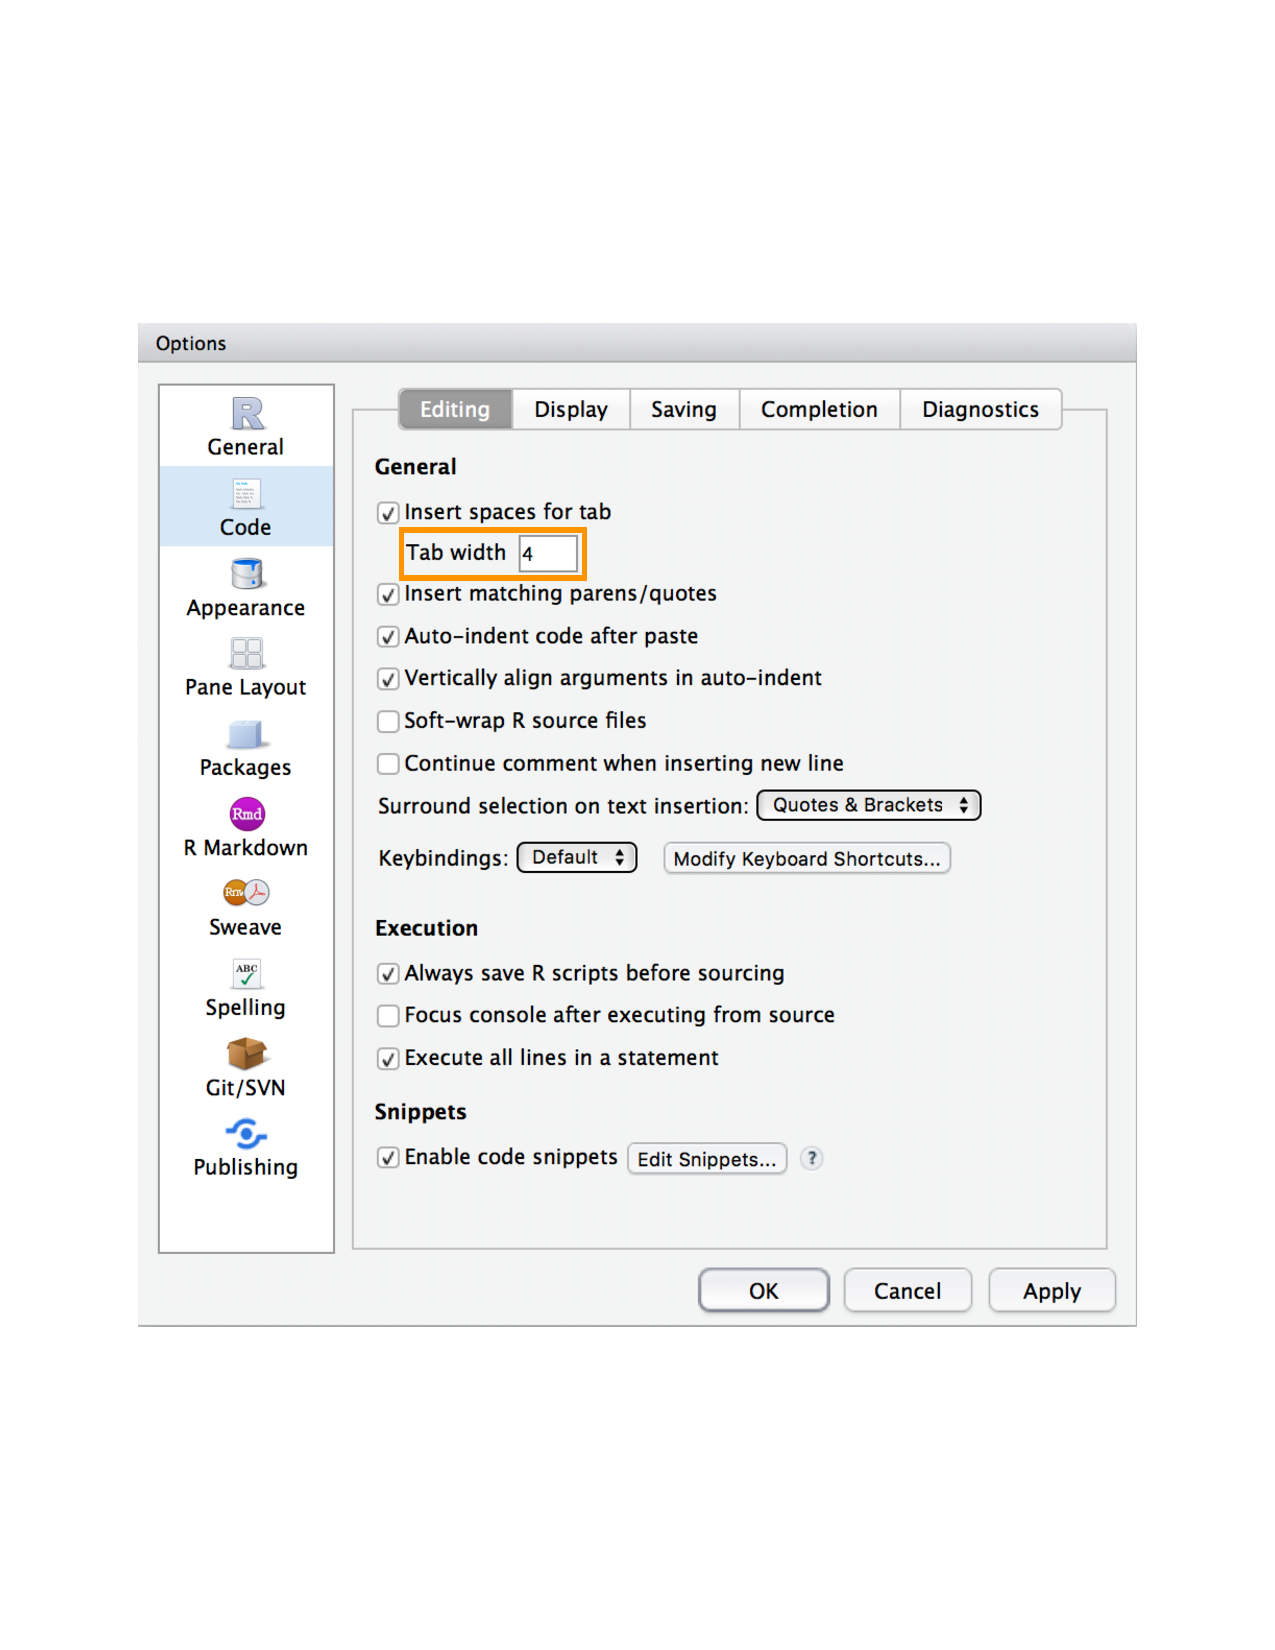
\includegraphics{rstudio-tab-width}
    \caption{Configuration de RStudio pour indenter le code de quatre
      caractères}
    \label{fig:collaboration:rstudio-tab-width}
  \end{figure}
\end{exercice}

\begin{exercice}
  Présenter le code ci-dessous selon les normes d'espacement,
  d'indentation et de positionnement des accolades mentionnées à la
  \autoref{sec:collaboration:presentation}. Pour ajuster
  automatiquement l'indentation avec RStudio, sélectionner le bloc de
  code et choisir dans les menus \code{Code|Reformat Code}.

\begin{Schunk}
\begin{Verbatim}
f <- function(x){
  if(all(x>=0)|| all(x<=0))
  { stop("all x are the same sign")
  }
  if (sum(diff(sign(x[x!=0]))!=0)>1)
  warning("more than one sign change")
 r<-polyroot(x)
i<-1/Re(r)[abs(Im(r))< .Machine$double.eps^0.5]-1
i[i > -1]
}
\end{Verbatim}
\end{Schunk}
\begin{sol}
  La présentation correcte comporte des espaces autour de tous les
  opérateurs, une indentation de quatre (4) caractères et des
  accolades ouvrante et fermante placées sur leur propre ligne.
\begin{Schunk}
\begin{Verbatim}
tri <- function(x)
{
    if (all(x >= 0) || all(x <= 0))
    {
        stop("all x are the same sign")
    }
    if (sum(diff(sign(x[x != 0])) != 0) > 1)
        warning("more than one sign change")
    r <- polyroot(x)
    i <- 1/Re(r)[abs(Im(r)) < .Machine$double.eps^0.5] - 1
    i[i > -1]
}
\end{Verbatim}
\end{Schunk}
\end{sol}
\end{exercice}

\begin{exercice}[nosol]
  Suivre le tutoriel interactif \link{https://try.github.io/}{tryGit}
  pour vous familiariser avec les commandes principales de Git.
\end{exercice}

\begin{exercice}
  Créer un compte chez \link{https://github.com}{GitHub}, puis créer
  un «embranchement» (\emph{fork}) du projet test
  \link{https://github.com/octocat/Spoon-Knife}{Spoon-Knife} depuis
  l'interface graphique de GitHub. Vous disposerez alors d'une copie
  de ce projet dans vos propres projets. Effectuer ensuite les
  opérations suivantes.
  \begin{enumerate}
  \item Cloner le projet sur votre poste de travail.
  \item Créer une branche locale pour effectuer une modification au
    projet.
  \item Modifier le fichier \code{index.html} d'une manière
    quelconque.
  \item Publier localement la modification dans la branche.
  \item Publier la branche dans le dépôt GitHub.
  \item Effectuer une «demande de tirage» (\emph{pull request}) dans
    le projet original à partir de l'interface de GitHub. Comme il
    s'agit d'un dépôt test, elle sera ignorée.
  \end{enumerate}

  \begin{sol}
    Pour créer l'embranchement (\emph{fork}), il suffit d'appuyer sur
    le bouton \code{Fork} en haut à droite de la page
    \link{https://github.com/octocat/Spoon-Knife}{Spoon-Knife}.
    Ensuite, les commandes à exécuter depuis une ligne de commande Git
    Bash (Windows) ou Terminal (macOS) sont les suivantes, dans
    l'ordre:
\begin{Schunk}
\begin{Verbatim}[commandchars=\\\{\}]
git clone https://github.com/\meta{username}/Spoon-Knife.git
cd Spoon-Knife
git checkout -b \meta{nom_branche}
\meta{modifier le fichier index.html avec son éditeur}
git status
git add index.html
git commit -m "\meta{message}"
git push -u origin \meta{nom_branche}
\end{Verbatim}
\end{Schunk}
    Enfin, retourner sur la page du projet d'origine et appuyer sur le
    bouton \code{Compare \& pull request} et suivre les instructions.
    Votre demande de tirage devrait ensuite apparaitre dans la liste
    de toutes les demandes du projet (plus de \nombre{5000} au moment
    d'écrire ces lignes).
  \end{sol}
\end{exercice}

\Closesolutionfile{solutions}


%%% Local Variables:
%%% mode: latex
%%% TeX-engine: xetex
%%% TeX-master: "programmer-avec-r"
%%% coding: utf-8
%%% End:

%%% Copyright (C) 2017 Vincent Goulet
%%%
%%% Ce fichier fait partie du projet «Programmer avec R»
%%% http://github.com/vigou3/programmer-avec-r
%%%
%%% Cette création est mise à disposition selon le contrat
%%% Attribution-Partage dans les mêmes conditions 4.0
%%% International de Creative Commons.
%%% http://creativecommons.org/licenses/by-sa/4.0/

\chapter{Analyse et contrôle de texte}
\label{chap:texte}

\begin{objectifs}
\item Déterminer si une chaine de caractères correspond ou non à une
  expression régulière donnée.
\item Écrire une expression régulière correspondant à une chaine de
  caractères donnée.
\item Identifier les lignes d'un fichier de texte ayant des propriétés
  communes à l'aide de \code{grep}.
\item Rechercher et remplacer des chaines de caractères ayant des
  propriétés communes à l'aide de \code{sed}.
\item Effectuer les opérations précédentes sur des chaînes de
  caractères divisées en champs logiques avec \code{awk}.
\item Effectuer les opérations de recherche et de remplacement de
  texte à l'aide d'expressions régulières avec les divers outils de R.
\end{objectifs}


Peut-être vous êtes-vous déjà demandé comment s'effectue la validation
de certains champs comme le code postal ou l'adresse de courrier
électronique dans les formulaires électroniques. Sûrement pas en
vérifiant si l'entrée figure dans la liste des quelques 17,5 millions
de codes postaux possibles ou, pire, parmi les milliards d'adresse de
courriel que les \link{https://tools.ietf.org/html/rfc3696}{règles
  internationales} permettent de concevoir! Non, ce qu'il faut, c'est
un «langage» qui permet de décrire \emph{comment} une chaine de
caractères peut être composée, sans toutefois en fixer la composition
exacte. Un tel langage existe: ce sont les \emph{expressions
  régulières} ou expressions relationnelles.

Une expression régulière (\emph{regular expression}, ou regex ou
regexp) est une chaine de caractères qui décrit, selon une syntaxe
précise, un ensemble de chaines de caractères possibles
\citep{Wikipedia:Expression_reguliere}.

Par exemple, les plaques d'immatriculation récentes distribuées par la
Société d'assurance automobile du Québec (SAAQ) sont composées ainsi:
une lettre, deux chiffres, une espace, trois lettres. Les lettres
\textsf{O}, \textsf{I} et \textsf{U} ne sont pas utilisées à cause de
leur similitude avec, respectivement, les chiffres {\fullcaps 0} et
{\fullcaps 1} et la lettre \textsf{V}. L'expression régulière suivante
permet de décrire l'ensemble des numéros de plaques possibles (y
compris les combinaisons de lettres exclues comme \code{LSD} ou
\code{SEX}):
\begin{Schunk}
\begin{Verbatim}
[A-HJ-NP-TV-Z][0-9]{2} [A-HJ-NP-TV-Z]{3}
\end{Verbatim}
\end{Schunk}

Voici quelques autres utilisations possibles des expressions
régulières.
\begin{itemize}
\item Rechercher du texte pouvant contenir des variations ou des
  fautes d'orthographe comme, par exemple, «je transfert» plutôt que
  «je transfère», ou encore les multiples variations autour du verbe
  «appeler»: appel, appelle, appellent, appeler, appelez, etc.
\item Remplacer le nom d'une commande par un autre lorsque la commande
  s'étend de part et d'autre d'un argument qui, lui, change d'une fois
  à l'autre. Par exemple, dans le système de mise en page {\LaTeX}, la
  syntaxe des commandes est la suivante:
  \cmdprint{\cmd}\oarg{option}\marg{arg}. Pour remplacer toutes les
  utilisations d'une commande \cmdprint{\foo} par \cmdprint{\bar}, il
  faut pouvoir tenir compte de la présence possible d'un argument
  optionnel \oarg{option} ainsi que de l'argument \marg{arg} qui
  change d'une utilisation de la commande à une autre.
\item Extraire les coordonnées géographiques d'un lieu (latitude et
  longitude) de l'URL d'une carte Google Maps. Par exemple, l'%
  \link{https://www.google.ca/maps/place/Universite+Laval/@46.7817463,-71.2769311,17z/data=!3m1!4b1!4m5!3m4!1s0x4cb896c469ff32f9:0x15feb853bd2f8247!8m2!3d46.7817463!4d-71.2747424}{URL
    correspondant} à la recherche «Université Laval» est
  \begin{Schunk}
\begin{Verbatim}
https://www.google.ca/maps/place/Universite+Laval/
  @46.7817463,-71.2769311,17z/data=!3m1!4b1!4m5!3m4!
  1s0x4cb896c469ff32f9:0x15feb853bd2f8247!8m2!3d
  46.7817463!4d-71.2747424
\end{Verbatim}
  \end{Schunk}
  dont on décode que le lieu se trouve à une latitude de
  $\nombre{46,7817463}$ et à une longitude de $\nombre{-71.2769311}$
  en degrés décimaux.
\end{itemize}

Un jour ou l'autre, vous aurez à traiter des chaines de caractères en
programmation ou en analyse de données. Ce jour-là, connaitre les
expressions régulières vous sauvera énormément de temps.


\section{Outils d'analyse et de contrôle du texte}
\label{sec:texte:outils}

L'expression régulière ne constitue qu'un langage de description d'une
chaine de texte. Pour exploiter ce langage, des outils sont
nécessaires. Aux fins de cet ouvrage, j'ai choisi de concentrer notre
étude sur les utilitaires Unix standards en ligne de commande
\code{grep}, \code{sed} et \code{awk}. Ils font partie intégrante des
systèmes d'exploitation macOS et Linux et, sous Windows, ils sont
livrés avec les interpréteurs de commande MSYS de \index{MSYS2}MSYS2
et \index{Git~Bash}Git~Bash de \emph{Git for Windows} dont nous avons
déjà parlé à la \autoref{sec:informatique:cli}.

Comme la plupart des utilitaires Unix, \Icode{grep}, \Icode{sed} et
\Icode{awk} prennent en entrée un flux de texte ou un ou plusieurs
fichiers en format texte brut et ils opèrent sur cette entrée ligne
par ligne. Le résultat du traitement est affiché à la ligne de
commande, envoyé à un autre programme ou redirigé vers un fichier. Les
outils diffèrent quant au type de traitement qu'ils peuvent effectuer.
\begin{description}
\item[\code{grep}] sélectionne les lignes en entrée correspondant à
  une expression régulière;
\item[\code{sed}] sert surtout pour rechercher et remplacer du texte;
\item[\code{awk}] permet de traiter aisément du texte séparé en champs
  ainsi que du texte réparti sur plusieurs lignes.
\end{description}

\warningbox{Il existe plusieurs versions différentes de ces outils,
  parfois avec des différences importantes, notamment en ce qui a
  trait à \code{sed}. Les versions sous Linux, \index{MSYS2}MSYS2 et
  \index{Git~Bash}Git~Bash sont généralement celles du
  \link{https://www.gnu.org/}{projet GNU}. Dans macOS, elles
  proviennent de
  \link{https://en.wikipedia.org/wiki/Berkeley_Software_Distribution}{BSD}.}


\section{Transfert de données et redirection}
\label{sec:texte:flux}

Parce qu'ils sont souvent utilisés avec les outils \icode{grep},
\icode{sed} et \icode{awk}, il convient, avant d'aller plus loin, de
dire un mot sur les opérateurs de transfert de données et de
redirection de \index{Unix}Unix.

Les programmes Unix en ligne de commande reçoivent leurs données d'une
\Index{entree standard@entrée standard}\Index{Unix!entree
  standard@entrée standard}\emph{entrée standard} (\emph{standard
  input}, souvent abrégé en \emph{stdin}) et renvoient leurs résultats
vers la \Index{sortie standard}\Index{Unix!sortie
  standard}\emph{sortie standard} (\emph{standard output},
\emph{stdout}). Pour simplifier, l'entrée standard d'un terminal
serait le clavier et la sortie standard, l'écran.

L'opérateur de transfert de données %
\index{{"|}@\code{\textbar} (Bash)|bfhyperpage} «\code{\textbar}»
(nommé «tuyau», de l'anglais \emph{pipe}) permet de
transférer la sortie d'un programme directement à l'entrée d'un autre
programme. Autrement dit, plutôt que d'afficher ses résultats à
l'écran, le premier programme les passe en entrée au second programme.

L'opérateur de redirection %
\index{>@\code{>} (Bash)|bfhyperpage}«\code{>}» permet, lui, de
rediriger la sortie d'un programme vers un fichier afin de sauvegarder
les résultats. Si le fichier existe déjà, son contenu est écrasé pour
le nouveau contenu. Pour ajouter le nouveau contenu à la fin du
fichier, il faut utiliser la variante double %
\index{>>@\code{>>} (Bash)|bfhyperpage}«\code{>>}» de l'opérateur de
redirection.

Enfin, l'opérateur de redirection %
\Index{>@\code{<} (Bash)}«\code{<}» permet, à l'inverse du précédent,
de déverser le contenu d'un fichier dans l'entrée standard d'un
programme. La variante double existe également.

La documentation citée en référence à la section suivante utilise
abondamment les opérateurs ci-dessus.


\section{Expressions régulières}
\label{sec:texte:regex}

Il existe une multitude de tutoriels et de documents de référence sur
les expressions régulières et sur les utilitaires \icode{grep},
\icode{sed} et \icode{awk}, que ce soit dans Internet ou sous forme de
livre. Or, le guide \link{https://developer.apple.com/library/content/documentation/OpenSource/Conceptual/ShellScripting/}{\emph{Shell Scripting Primer}} de la bibliothèque
pour développeurs de Apple \citep{Apple:shellprimer} s'avère une
référence idéale pour vous accompagner dans l'atteinte des objectifs
d'apprentissage mentionnés au début du chapitre.

\windowsbox{Utilisateurs de Windows: pas de souci! Bien qu'émanant de
  Apple, le guide traite de procédures et d'outils Unix standards,
  outils dont vous disposez si vous avez installé \index{Git}\emph{Git
    for Windows} ou MSYS2\index{MSYS2}, tel qu'expliqué à la
  \autoref{sec:informatique:cli:windows}.}

Je vous invite donc à étudier les chapitres suivants du guide
\emph{Shell Scripting Primer}:
\begin{itemize}
\item
  \link{https://developer.apple.com/library/content/documentation/OpenSource/Conceptual/ShellScripting/RegularExpressionsUnfettered/RegularExpressionsUnfettered.html}{\emph{Regular
      Expressions Unfettered}} jusqu'à la section \emph{Using
    Modifiers}, inclusivement.
\item
  \link{https://developer.apple.com/library/content/documentation/OpenSource/Conceptual/ShellScripting/Howawk-ward/Howawk-ward.html}{\emph{How
      AWK-ward}} jusqu'à la section \emph{Changing the Record and
    Field Separators in AWK Scripts}, inclusivement.
\end{itemize}
Revenez ensuite ici pour des exemples additionnels et des exercices.

\warningbox{Vous pouvez ignorer toutes les notions relatives à Perl
  exposées dans \emph{Shell Scripting Primer}.}


\section{Exemples additionnels}
\label{sec:texte:exemples}

Exceptionnellement, je présente les exemples additionnels de ce
chapitre en texte normal plutôt que sous forme de fichier de script.

Les exemples ci-dessous utilisent des fichiers distribués avec le
présent document dans l'archive \code{programmer-avec-r.zip}.
Assurez-vous d'avoir extrait les fichiers de l'archive quelque part
sur votre disque et notez bien cet endroit: vous en aurez besoin dans
un instant.

Vous devez entrer les expressions ci-dessous à une ligne de commande
du \index{Terminal}Terminal sous macOS, ou de \index{Git~Bash}Git~Bash
ou MSYS sous Windows.

\importantbox{L'espace horizontal étant compté dans un document en
  format PDF, il est parfois nécessaire de scinder une commande sur
  deux lignes ou plus. Pour ces cas, j'ai inséré le symbole de
  continuation de ligne «\bs» de Bash à la fin des lignes. Vous pouvez
  ainsi copier les commandes directement du document et les coller
  dans une ligne de commande. Le symbole {\bs} ne fait \emph{pas}
  partie des commandes.}

En premier lieu, déplacez, à l'aide de la commande \icode{cd},
l'invite de commande dans le répertoire où vous avez extrait les
fichiers de l'archive.

Comme premier exemple, dressons la liste de toutes les utilisations de
la fonction \code{matrix} dans les fichiers d'exemples. C'est un
travail pour l'utilitaire \icode{grep}.
\begin{Schunk}
\begin{Verbatim}
$ grep matrix *.R
\end{Verbatim}
\end{Schunk}

L'option \code{-l} de \icode{grep} permet de limiter les résultats à
la liste des fichiers contenant au moins une utilisation de
\code{matrix}.
\begin{Schunk}
\begin{Verbatim}
$ grep -l matrix *.R
\end{Verbatim}
\end{Schunk}

La commande suivante permet de savoir quel fichier d'exemples traite
de la suite de Fibonacci.
\begin{Schunk}
\begin{Verbatim}
$ grep -l fibonacci *.R
\end{Verbatim}
\end{Schunk}

Pour connaitre les fichiers d'exemples dans lesquels apparaissent les
objets \code{letters} et \code{LETTERS}, nous devons rechercher sans
égard à la casse pour attraper les deux cas.
\begin{Schunk}
\begin{Verbatim}
$ grep -i letters *.R
\end{Verbatim}
\end{Schunk}

Allons-y maintenant d'une expression régulière plus élaborée pour
trouver toutes les utilisations de la fonction \code{g} dans les
fichiers d'exemples, c'est-à-dire la chaine \code{g(} précédée d'au
moins une espace ou en début de ligne.
\begin{Schunk}
\begin{Verbatim}
$ grep -E '( |^)g\(' *.R
\end{Verbatim}
\end{Schunk}

Tel que mentionné à la \autoref{sec:texte:outils}, la fonction
\icode{sed} sert surtout pour rechercher et remplacer dans un fichier,
et ce, ligne par ligne par défaut. Remplaçons les symboles de
commentaires triples \code{\#\#\#} en début de ligne (à la Emacs) dans
le fichier \code{implementation.R} par un symbole unique \code{\#} (à
la RStudio). Pour faire bonne mesure, plaçons le résultat dans un
nouveau fichier \code{implementation-new.R} à l'aide de l'opérateur de
redirection \index{>@\code{>} (Bash)}\code{>}.
\begin{Schunk}
\begin{Verbatim}
$ sed 's/^###/#/' implementation.R > implementation-new.R
\end{Verbatim}
\end{Schunk}

Le programme \icode{awk} est particulièrement utile pour traiter des
fichiers dont les lignes sont séparés en «champs», comme des colonnes
de données, par exemple. Or, le présent document est justement livré
avec le fichier \code{100metres.data} qui contient la liste des 31
meilleurs temps enregistrés au 100~mètres homme entre 1964 et 2005
(voir l'\autoref{ex:internes:100metres}). La commande \Icode{cat}
permet d'afficher le contenu du fichier sur la sortie standard.
\begin{Schunk}
\begin{Verbatim}
$ cat 100metres.data
\end{Verbatim}
\end{Schunk}

Effectuons dans un premier temps l'extraction des temps des records
(second champ). La première commande utilise un transfert de données
du programme \icode{cat} vers \icode{awk} avec l'opérateur %
\index{{"|}@\code{\textbar} (Bash)}\code{\textbar}, alors
que la seconde, plus usuelle et tout à fait équivalente, emploie un
fichier en entrée.
\begin{Schunk}
\begin{Verbatim}
$ cat 100metres.data | awk '{ print $2 }'
$ awk '{ print $2 }' 100metres.data
\end{Verbatim}
\end{Schunk}

L'inversion des deux colonnes du fichier est simple à réaliser avec
\icode{awk}.
\begin{Schunk}
\begin{Verbatim}
$ awk '{ print $2, $1 }' 100metres.data
\end{Verbatim}
\end{Schunk}

Les colonnes du fichier \code{100metres.data} sont séparées par une
espace. Remplaçons ces espaces par des virgules pour convertir le
fichier en format CSV. Je fournis deux solutions, avec \icode{awk} et avec
\icode{sed}.
\begin{Schunk}
\begin{Verbatim}
$ awk '{ print $1","$2 }' 100metres.data
$ sed 's/ /,/' 100metres.data
\end{Verbatim}
\end{Schunk}

Changeons maintenant le format de la date du format
\link{https://fr.wikipedia.org/wiki/ISO_8601}{ISO~8601} aaaa-mm-qq
vers le format américain qq/mm/aa. D'abord une solution avec
\icode{awk}. En premier lieu, nous devons changer le séparateur de
champs de \code{awk} (l'espace par défaut) pour l'espace et le tiret.
Ainsi, \code{awk} va non seulement séparer les deux colonnes du
fichier, mais aussi les champs de la date. Ensuite, nous replaçons les
champs dans l'ordre voulu avec les bons séparateurs. La fonction
\index{substr@\code{substr} (awk)}\code{substr} de \code{awk} permet
de sélectionner une partie d'une chaine de caractères
\citep[section~9.1.3]{awk}.
\begin{Schunk}
\begin{Verbatim}
$ awk 'BEGIN { FS = "[ -]" } \
       { print $2"/"$3"/"substr($1, 3), $4 }' \
       100metres.data
\end{Verbatim}
\end{Schunk}

La solution avec \icode{sed} maintenant, qui repose non pas sur des
champs détectés automatiquement, mais plutôt sur la recherche et le
remplacement d'expressions régulières. Nous recherchons l'expression
régulière suivante en capturant chaque élément trouvé (sauf les
tirets): les nombres 19 ou 20; deux chiffres; un tiret; deux chiffres;
un tiret; deux chiffres; tout le reste de la ligne. Nous replaçons
ensuite les éléments capturés dans l'ordre souhaité avec des barres
obliques \code{/} entre les éléments de dates. Comme le symbole
\code{/} est utilisé dans la chaine de sortie, il faut utiliser un
autre symbole pour séparer les champs de la commande \code{sed}. J'ai
utilisé le symbole \code{~} ici.
\begin{Schunk}
\begin{Verbatim}
$ sed -E 's~(19|20)([0-9]{2})-([0-9]{2})-([0-9]{2})(.*)~'\
'\3/\4/\2\5~' 100metres.data
\end{Verbatim}
\end{Schunk}

Amusons-nous maintenant avec le fichier \code{README.md} qui contient,
regroupées à la fin du fichier, les notes de mise à jour des différentes
versions du document. Les deux commandes suivantes dressent la liste
des numéros de versions avec les variantes de base et étendue
des expressions régulières.
\begin{Schunk}
\begin{Verbatim}
$ grep '^### [[:digit:]]' README.md
$ grep -E '^#{3} [[:digit:]]' README.md
\end{Verbatim}
\end{Schunk}

Terminons avec deux exemples plus avancés. Nous souhaitons d'abord
extraire tout l'historique des versions du fichier \code{README.md}.
Cet historique se trouve à la fin du fichier, à partir de la ligne
débutant par la chaine \code{\#\# Historique}. Le meilleur outil pour
effectuer des opérations sur plusieurs lignes d'un fichier est
\icode{awk}, tel que mentionné à la \autoref{sec:texte:outils}.
L'idée, ici, est la suivante: lorsque la chaine est trouvée, donner
une valeur de 1 (vrai) à une variable d'«état», puis afficher les
lignes lorsque la variable est vraie (donc toutes celles qui suivent).
Je présente deux versions de la commande, une explicite et une plus
compacte.
\begin{Schunk}
\begin{Verbatim}
$ awk '/^## Historique/ { state = 1; next } \
       state == 1 { print }' README.md
$ awk '/^## Historique/ { state = 1; next } \
       state' README.md
\end{Verbatim}
\end{Schunk}

\tipbox{Explication de la version compacte: écrire \code{state == 1}
  pour tester que la variable \code{state} est vraie n'est pas
  nécessaire dans la mesure où il est sous-entendu que l'expression
  qui précède l'action dans une commande \icode{awk} est un test
  conditionnel et que \code{awk} traite la valeur 1 comme vraie. De
  plus, la commande \code{print} est implicite avec \code{awk}, donc
  il n'est pas nécessaire de la demander explicitement.}

Ensuite, nous voulons extraire seulement les notes de mise à jour de
la \emph{dernière} version du document. L'idée consiste à afficher les lignes
du fichier à partir de la première section marquée par \code{\#\#\#} après
\code{\#\# Historique} et d'arrêter lorsqu'une autre section marquée par
\code{\#\#\#} est atteinte. Ces opérations nécessitent deux valeurs de la
variable d'état \code{state}.
\begin{Schunk}
\begin{Verbatim}
$ awk '/^## Historique/ { state = 1 } \
       (state == 1) && /^### / { state = 2; next } \
       (state == 2) && /^### / { exit } \
       state == 2 { print }' README.md
\end{Verbatim}
\end{Schunk}

\notebox{Les opérations de composition du présent document, de
  publication dans GitHub et de mise à jour de la page web sont
  entièrement automatisées à l'aide de
  \link{https://fr.wikipedia.org/wiki/Make}{\code{make}}, un autre de
  ces outils standards sur les systèmes Unix. Vous pouvez retrouver
  une variante un peu plus élaborée de la commande \code{awk}
  ci-dessus dans la règle \code{create-release} du fichier de
  configuration \code{Makefile} qui se trouve dans le
  \link{\ghurl}{code source} du document.}

\section{Exercices}
\label{sec:texte:exercices}

\Opensolutionfile{solutions}[solutions-texte]

\begin{Filesave}{solutions}
\section*{Chapitre \ref*{chap:texte}}
\addcontentsline{toc}{section}{Chapitre \protect\ref*{chap:texte}}

\end{Filesave}


\begin{exercice}
  Dans chacun des cas ci-dessous, déterminer à laquelle ou lesquelles
  des chaines de caractères correspond l'expression régulière donnée.
  Les symboles \verb=/= ne servent qu'à délimiter le début et la fin
  des expressions régulières. Ne pas tenir compte des espaces avant ou
  après les chaines.\footnote{%
    Exercice adapté de
    \url{https://regex.sketchengine.co.uk/extra_regexps.html}.}
  \begin{enumerate}
    \setlength{\multicolsep}{2pt}
  \item \verb~/a(ab)*a/~
    \begin{enumerate}[1)]
      \begin{multicols}{3}
      \item \verb~abababa~
      \item \verb~aaba~
      \item \verb~aabbaa~
      \end{multicols}
      \begin{multicols}{3}
      \item \verb~aba~
      \item \verb~aabababa~
      \end{multicols}
    \end{enumerate}
  \item \verb~/ab+c?/~
    \begin{enumerate}[1)]
      \begin{multicols}{3}
      \item \verb~abc~
      \item \verb~ac~
      \item \verb~abbb~
      \end{multicols}
      \begin{multicols}{3}
      \item \verb~bbc~
      \item \verb~abcc~
      \end{multicols}
    \end{enumerate}
  \item \verb~/a.[bc]+/~
    \begin{enumerate}[1)]
      \begin{multicols}{3}
      \item \verb~abc~
      \item \verb~abbbbbbbb~
      \item \verb~azc~
      \end{multicols}
      \begin{multicols}{3}
      \item \verb~abcbcbcbc~
      \item \verb~ac~
      \item \verb~asccbbbbcbcccc~
      \end{multicols}
    \end{enumerate}
  \item \verb~/abc|xyz/~
    \begin{enumerate}[1)]
      \begin{multicols}{3}
      \item \verb~abc~
      \item \verb~xyz~
      \item \verb~abc|xyz~
      \end{multicols}
    \end{enumerate}
  \item \verb~/[a-z]+[\.\?!]/~
    \begin{enumerate}[1)]
      \begin{multicols}{3}
      \item \verb~battle!~
      \item \verb~Hot~
      \item \verb~green~
      \end{multicols}
      \begin{multicols}{3}
      \item \verb~swamping.~
      \item \verb~jump up.~
      \item \verb~undulate?~
      \end{multicols}
      \begin{multicols}{3}
      \item \verb~is.?~
      \end{multicols}
    \end{enumerate}
  \item \verb~/[a-zA-Z]*[^,]=/~
    \begin{enumerate}[1)]
      \begin{multicols}{3}
      \item \verb~Butt=~
      \item \verb~BotHEr,=~
      \item \verb~Ample~
      \end{multicols}
      \begin{multicols}{3}
      \item \verb~FIdDlE7h=~
      \item \verb~Brittle =~
      \item \verb~Other.=~
      \end{multicols}
    \end{enumerate}
  \item \verb~/[a-z][\.\?!]\s+[A-Z]/~
    \begin{enumerate}[1)]
      \begin{multicols}{3}
      \item \verb~A. B~
      \item \verb~c! d~
      \item \verb~e f~
      \end{multicols}
      \begin{multicols}{3}
      \item \verb~g. H~
      \item \verb~i? J~
      \item \verb~k L~
      \end{multicols}
    \end{enumerate}
  \item \verb~/<[^>]+>/~
    \begin{enumerate}[1)]
      \begin{multicols}{2}
      \item \verb~<an xml tag>~
      \item \verb~<opentag> <closetag>~
      \end{multicols}
      \begin{multicols}{2}
      \item \verb~</closetag>~
      \item \verb~<>~
      \end{multicols}
      \begin{multicols}{2}
      \item \verb~<with attribute=”77”>~
      \end{multicols}
    \end{enumerate}
  \end{enumerate}

  \begin{sol}
    \begin{enumerate}
    \item L'expression régulière recherche «\verb=a=», suivi zéro ou
      plusieurs occurrences de «\verb=ab=», suivi de «\verb=b=». Les
      choix 2 et 5 satisfont ces conditions.
    \item L'expression régulière recherche «\verb=a=», suivi d'au
      moins une occurrence de «\verb=b=», suivi de zéro ou une
      occurrence de «\verb=c=». Les choix 1 et 3 satisfont ces
      conditions.
    \item L'expression régulière recherche «\verb=a=», suivi d'un
      caractère quelconque (incluant «\verb=b=» ou «\verb=c=»), suivi
      d'au moins une occurrence de «\verb=b=» ou de «\verb=c=». Les
      choix 1, 2, 3, 4 et 6 satisfont ces conditions.
    \item L'expression régulière recherche «\verb=abc=» ou
      «\verb=xyz=». Les choix 1 et 2 satisfont la condition. Le
      troisième choix n'est pas valide puisque l'expression ne
      recherche pas le symbole «\verb=|=».
    \item L'expression régulière recherche au moins lettre minuscule
      (à l'exclusion de tout autre symbole), suivi de l'un ou l'autre
      des symboles «\verb=.=», «\verb=?=», «\verb=!=» (sans
      répétition). Les choix 1, 4 et 6 satisfont ces conditions.
    \item L'expression régulière recherche zéro ou plusieurs lettres
      minuscules ou majuscule (mais aucun autre symbole), suivi de
      tout autre caractère qu'une virgule, suivi du symbole
      «\verb|=|». Les choix 1, 5 et 6 satisfont ces conditions.
    \item L'expression régulière recherche une lettre minuscule, suivi
      de l'un ou l'autre des symboles «\verb=.=», «\verb=?=»,
      «\verb=!=» (sans répétition), suivi d'au moins une espace, suivi
      d'une lettre majuscule. Les choix 4 et 5 satisfont ces
      conditions.
    \item L'expression régulière recherche un symbole «\verb=<=»,
      suivi d'au moins symbole autre que «\verb=>=», suivi du symbole
      «\verb=>=». Les choix 1, 3 et 5 satisfont ces conditions.
    \end{enumerate}
  \end{sol}
\end{exercice}

\begin{exercice}
  Composer une expression régulière qui correspond à tous les mots de
  la liste de gauche, ci-dessous, mais à aucun des mots de la liste de
  droite.\footnote{%
    Exercice adapté de
    \url{https://regex.sketchengine.co.uk/cgi/ex1.cgi}.}
  \begin{center}
    \begin{minipage}[t]{0.3\linewidth}
      pit \\
      spot \\
      spate \\
      slap two \\
      respite
    \end{minipage}
    \begin{minipage}[t]{0.3\linewidth}
      pt \\
      Pot \\
      peat \\
      part
    \end{minipage}
  \end{center}
  \begin{sol}
    L'expression doit correspondre à la lettre minuscule «\verb=p=»
    précédée ou non d'une ou plusieurs lettres (ou symboles, ce n'est
    pas spécifié), suivie d'une (et une seule) lettre ou d'une espace,
    de la lettre «\verb=t=» et, enfin, de zéro ou de plusieurs
    lettres. Il y a assurément plusieurs réponses valides. En voici
    une: \verb=/.*p[a-z ]t.*/=.
  \end{sol}

\end{exercice}

\begin{exercice}
  Composer une expression régulière qui permet de vérifier la validité
  d'un code postal canadien dans un formulaire électronique. Ne pas
  tenir compte des règles précises de composition d'un code postal,
  mais bien seulement qu'il s'agit d'une suite de six caractères
  alternant entre une lettre et un chiffre. Les lettres peuvent être
  fournies en majuscule ou en minuscule et l'espace entre le troisième
  et le quatrième symbole peut être présent ou non.
  \begin{sol}
    \verb=[a-zA-z][0-9][a-zA-z]\s?[0-9][a-zA-z][0-9]= si l'on ne
    permet que zéro ou une espace entre les deux blocs. S'il n'y a pas
    de limite au nombre d'espaces, remplacer «\verb=?=» par
    «\verb=*=».
  \end{sol}
\end{exercice}

\begin{exercice}
  Écrire une commande \code{sed} permettant de changer le séparateur
  décimal dans les temps du fichier \code{100metres.data} pour une
  virgule.
  \begin{sol}
    \code{sed} est l'outil idéal pour de tels traitements simples à
    effectuer ligne par ligne.
    \begin{Schunk}
\begin{Verbatim}
$ sed 's/\./,/' 100metres.data
\end{Verbatim}
    \end{Schunk}
    Pour placer le fichier modifié dans, disons,
    \code{100metres-dec.data}, utiliser
    \begin{Schunk}
\begin{Verbatim}
$ sed 's/\./,/' 100metres.data > 100metres-dec.data
\end{Verbatim}
    \end{Schunk}
  \end{sol}
\end{exercice}

\begin{exercice}
  \begin{enumerate}
  \item Extraire du fichier \code{100metres.data} informations des
    temps réalisés au mois d'août.
  \item Extraire les informations des temps de moins de 10~secondes.
  \item Extraire les lignes du fichier satisfaisant les deux
    conditions ci-dessus. Vous pouvez utiliser l'opérateur de
    redirection \verb=|= de Unix (\autoref{sec:informatique:os:unix})
    pour combiner les deux commandes précédentes.
  \end{enumerate}
  \begin{sol}
    \begin{enumerate}
    \item C'est un travail pour \code{grep}. La solution la plus serait:
      \begin{Schunk}
\begin{Verbatim}
$ grep '-08-' 100metres.data
\end{Verbatim}
      \end{Schunk}
      Cependant, \code{grep} n'aime pas cette commande puisque le
      symbole \verb=-= est utilisé pour passer des options. Dans ce
      cas, il vaut mieux utiliser une option \verb=-e= pour déclarer
      explicitement à \code{grep} que ce qui suit est l'expression à
      rechercher:
      \begin{Schunk}
\begin{Verbatim}
$ grep -e '-08-' 100metres.data
\end{Verbatim}
      \end{Schunk}
      Autrement, simplement ajouter quelque chose à chercher avant le tiret:
      \begin{Schunk}
\begin{Verbatim}
$ grep '.*-08-' 100metres.data
\end{Verbatim}
      \end{Schunk}
    \item Le plus simple, ici, consiste à utiliser \code{awk} puisque
      les seconds champs --- les temps --- seront automatiquement
      disponibles.
      \begin{Schunk}
\begin{Verbatim}
$ awk '$2 < 10 { print }' 100metres.data
\end{Verbatim}
      \end{Schunk} %$
      Malheureusement, cette commande risque de ne pas fonctionner sur
      certains systèmes qui traitent la virgule comme le séparateur
      décimal, notamment les Mac en configuration française. Dans ce
      cas, essayer plutôt (j'ai supprimé la commande \verb={ print }=
      ci-dessous puisqu'elle est implicite):
      \begin{Schunk}
\begin{Verbatim}
$ LC_NUMERIC="en_US.UTF-8" awk '$2 < 10' 100metres.data
\end{Verbatim}
      \end{Schunk} %$
      Une solution avec \code{grep} consisterait à rechercher un
      «\verb=9.=» après l'espace sur chaque ligne:
      \begin{Schunk}
\begin{Verbatim}
$ grep ' 9\.' 100metres.data
\end{Verbatim}
      \end{Schunk}
    \item Nous pouvons combiner les deux commandes ainsi:
      \begin{Schunk}
\begin{Verbatim}
$ grep -e '-08-' 100metres.data | awk '$2 < 10'
\end{Verbatim}
      \end{Schunk} %$
      ou
      \begin{Schunk}
\begin{Verbatim}
$ grep -e '-08-' 100metres.data | grep ' 9\.'
\end{Verbatim}
      \end{Schunk}
    \end{enumerate}
  \end{sol}
\end{exercice}

\begin{exercice}
  Pour tous les appels à une fonction \code{f} comportant deux
  arguments dans le fichier \code{implementation.R} livré avec le
  présent document, changer le nom de la fonction pour \code{fun} et
  inverser l'ordre des deux arguments.
  \begin{sol}
    Ce traitement s'effectue bien avec \code{sed}:
    \begin{Schunk}
\begin{Verbatim}
$ sed -E 's/( |^)f\((.*), (.*)\)/fun(\3, \2)/' \
  implementation.R
\end{Verbatim}
    \end{Schunk}
    Le premier groupe \verb=( |^)= capture une espace avant \code{f}
    ou le début de la ligne.
  \end{sol}
\end{exercice}

\begin{exercice}
  Déterminer si la commande \code{print} est nécessaire ou non dans la
  toute dernière commande \icode{awk} de la
  \autoref{sec:texte:exemples}.
  \begin{sol}
    La commande \code{print} n'est pas nécessaire puisqu'il s'agit de
    l'action implicite dans \code{awk}.
  \end{sol}
\end{exercice}

\begin{exercice}
  Dans le code source du présent document\footnote{%
    Disponible en clonant avec Git le projet
    \url{https://projets.fsg.ulaval.ca/git/scm/vg/programmer-avec-r-develop.git}.}, %
  le fichier \code{docs/index.md} contient une ligne de ce type
  (affichée sur trois lignes ici pour des raisons de contraintes
  horizontales):
  \begin{Schunk}
\begin{Verbatim}
2017.11-2 ([notes de mise à jour]
  ({{ site.github.repository_url }}
  /releases/tag/v2017.11-2/))
\end{Verbatim}
  \end{Schunk}
  Le numéro de version du document apparait donc deux fois sur la
  ligne. Ce numéro de version est composé ainsi: année de publication;
  un point; mois de publication; une portion optionnelle composée d'un
  tiret, de un ou plusieurs chiffres et possiblement d'une lettre.
  Autrement dit, les chaines de caractères suivantes constituent
  toutes des numéros de versions valides: «2017.11», «2017.11-2»,
  «2017.11-2a», «2017.11-42k».

  Écrire une commande \code{sed} permettant de remplacer le numéro de
  version qui se trouverait actuellement dans le fichier
  \code{index.md}, quel qu'il fut, par le numéro de version
  2017.12-1a.
  \begin{sol}
    Invoquez \code{sed} avec l'option \code{-E} dans le cas présent
    pour utiliser les expressions régulières «étendues» ou modernes
    (l'opérateur \verb=?= n'existe pas dans la version de \code{sed}
    qui utilise les expressions de base sous macOS). À noter dans la
    réponse ci-dessous: l'expression régulière nécessaire et la
    présence de la commande \code{g} pour remplacer toutes les
    correspondances sur la ligne.
    \begin{Schunk}
\begin{Verbatim}
$ sed -E \
  's/[0-9]{4}\.[0-9]{2}(-[0-9]+[a-z]*)?/2017.12-1a/g' \
  index.md
\end{Verbatim}
    \end{Schunk}
    Le fichier \code{docs/Makefile} du projet contient une mise en
    œuvre avec \code{awk} équivalente, mais plus robuste.
  \end{sol}
\end{exercice}

\Closesolutionfile{solutions}

%%% Local Variables:
%%% mode: latex
%%% TeX-engine: xetex
%%% TeX-master: "programmer-avec-r"
%%% coding: utf-8
%%% End:

\include{debogage}
\include{oop}

\appendix
\chapter{RStudio: une introduction}
\index{RStudio|(}
\label{chap:rstudio}

Un environnement de développement intégré (\emph{integrated
  development environment}, IDE) est un progiciel de productivité
destiné au développement de logiciels ou, plus largement, à la
programmation informatique. Il comprend toujours un éditeur de texte
adapté au langage de programmation visé, un environnement de
compilation ou d'exécution du code et, généralement, des outils de
contrôle de versions, de gestion des projets et de navigation dans le
code source.\footnote{%
  À ce compte, GNU~Emacs constitue un environnement de développement
  intégré.} %

Offert au public depuis 2011, RStudio est un IDE convivial conçu
spécifiquement pour l'analyse de données et le développement de
packages avec R. Il est produit par RStudio~Inc.\ et est offert en
version libre ou commerciale, pour une exécution locale
(\emph{desktop}) ou pour une exécution sur un serveur via un
navigateur web.


\section{Installation}
\label{sec:rstudio:installation}

RStudio est disponible à l'identique pour les plateformes Windows,
macOS et Linux. Pour une utilisation locale sur son poste de travail,
on installera la version libre (\emph{Open Source}) de
\link{https://www.rstudio.com/products/rstudio/download/}{RStudio~Desktop}.


\section{Description sommaire}
\label{sec:rstudio:description}

La fenêtre de RStudio se divise toujours en quatre
sous-fenêtres\footnote{%
  Les sous-fenêtres sont appelées \emph{panes} (en anglais) dans
  l'application.} %
--- sauf au lancement, alors que la sous-fenêtre d'édition de code
source n'est pas visible; voir la \autoref{fig:rstudio:rstudiowindow}.
Dans le sens des aiguilles d'une montre en partant en haut à gauche,
on trouve:
\begin{enumerate}
  \index{RStudio!sous-fenêtres}
\item la sous-fenêtre d'édition de code source, avec un onglet par
  fichier de script;
\item le navigateur d'environnement de travail ou d'historique des
  commandes, selon l'onglet sélectionné;
\item le navigateur de fichiers du projet, de packages, de graphiques,
  etc., selon l'onglet sélectionné;
\item la console --- ou ligne de commande --- R.
\end{enumerate}
Au lancement de l'application, la console R occupe toute la gauche de
la fenêtre jusqu'à ce qu'un fichier de script soit ouvert.

\begin{figure}[t]
  %% Capture d'écran et espace additionnel sous l'image
  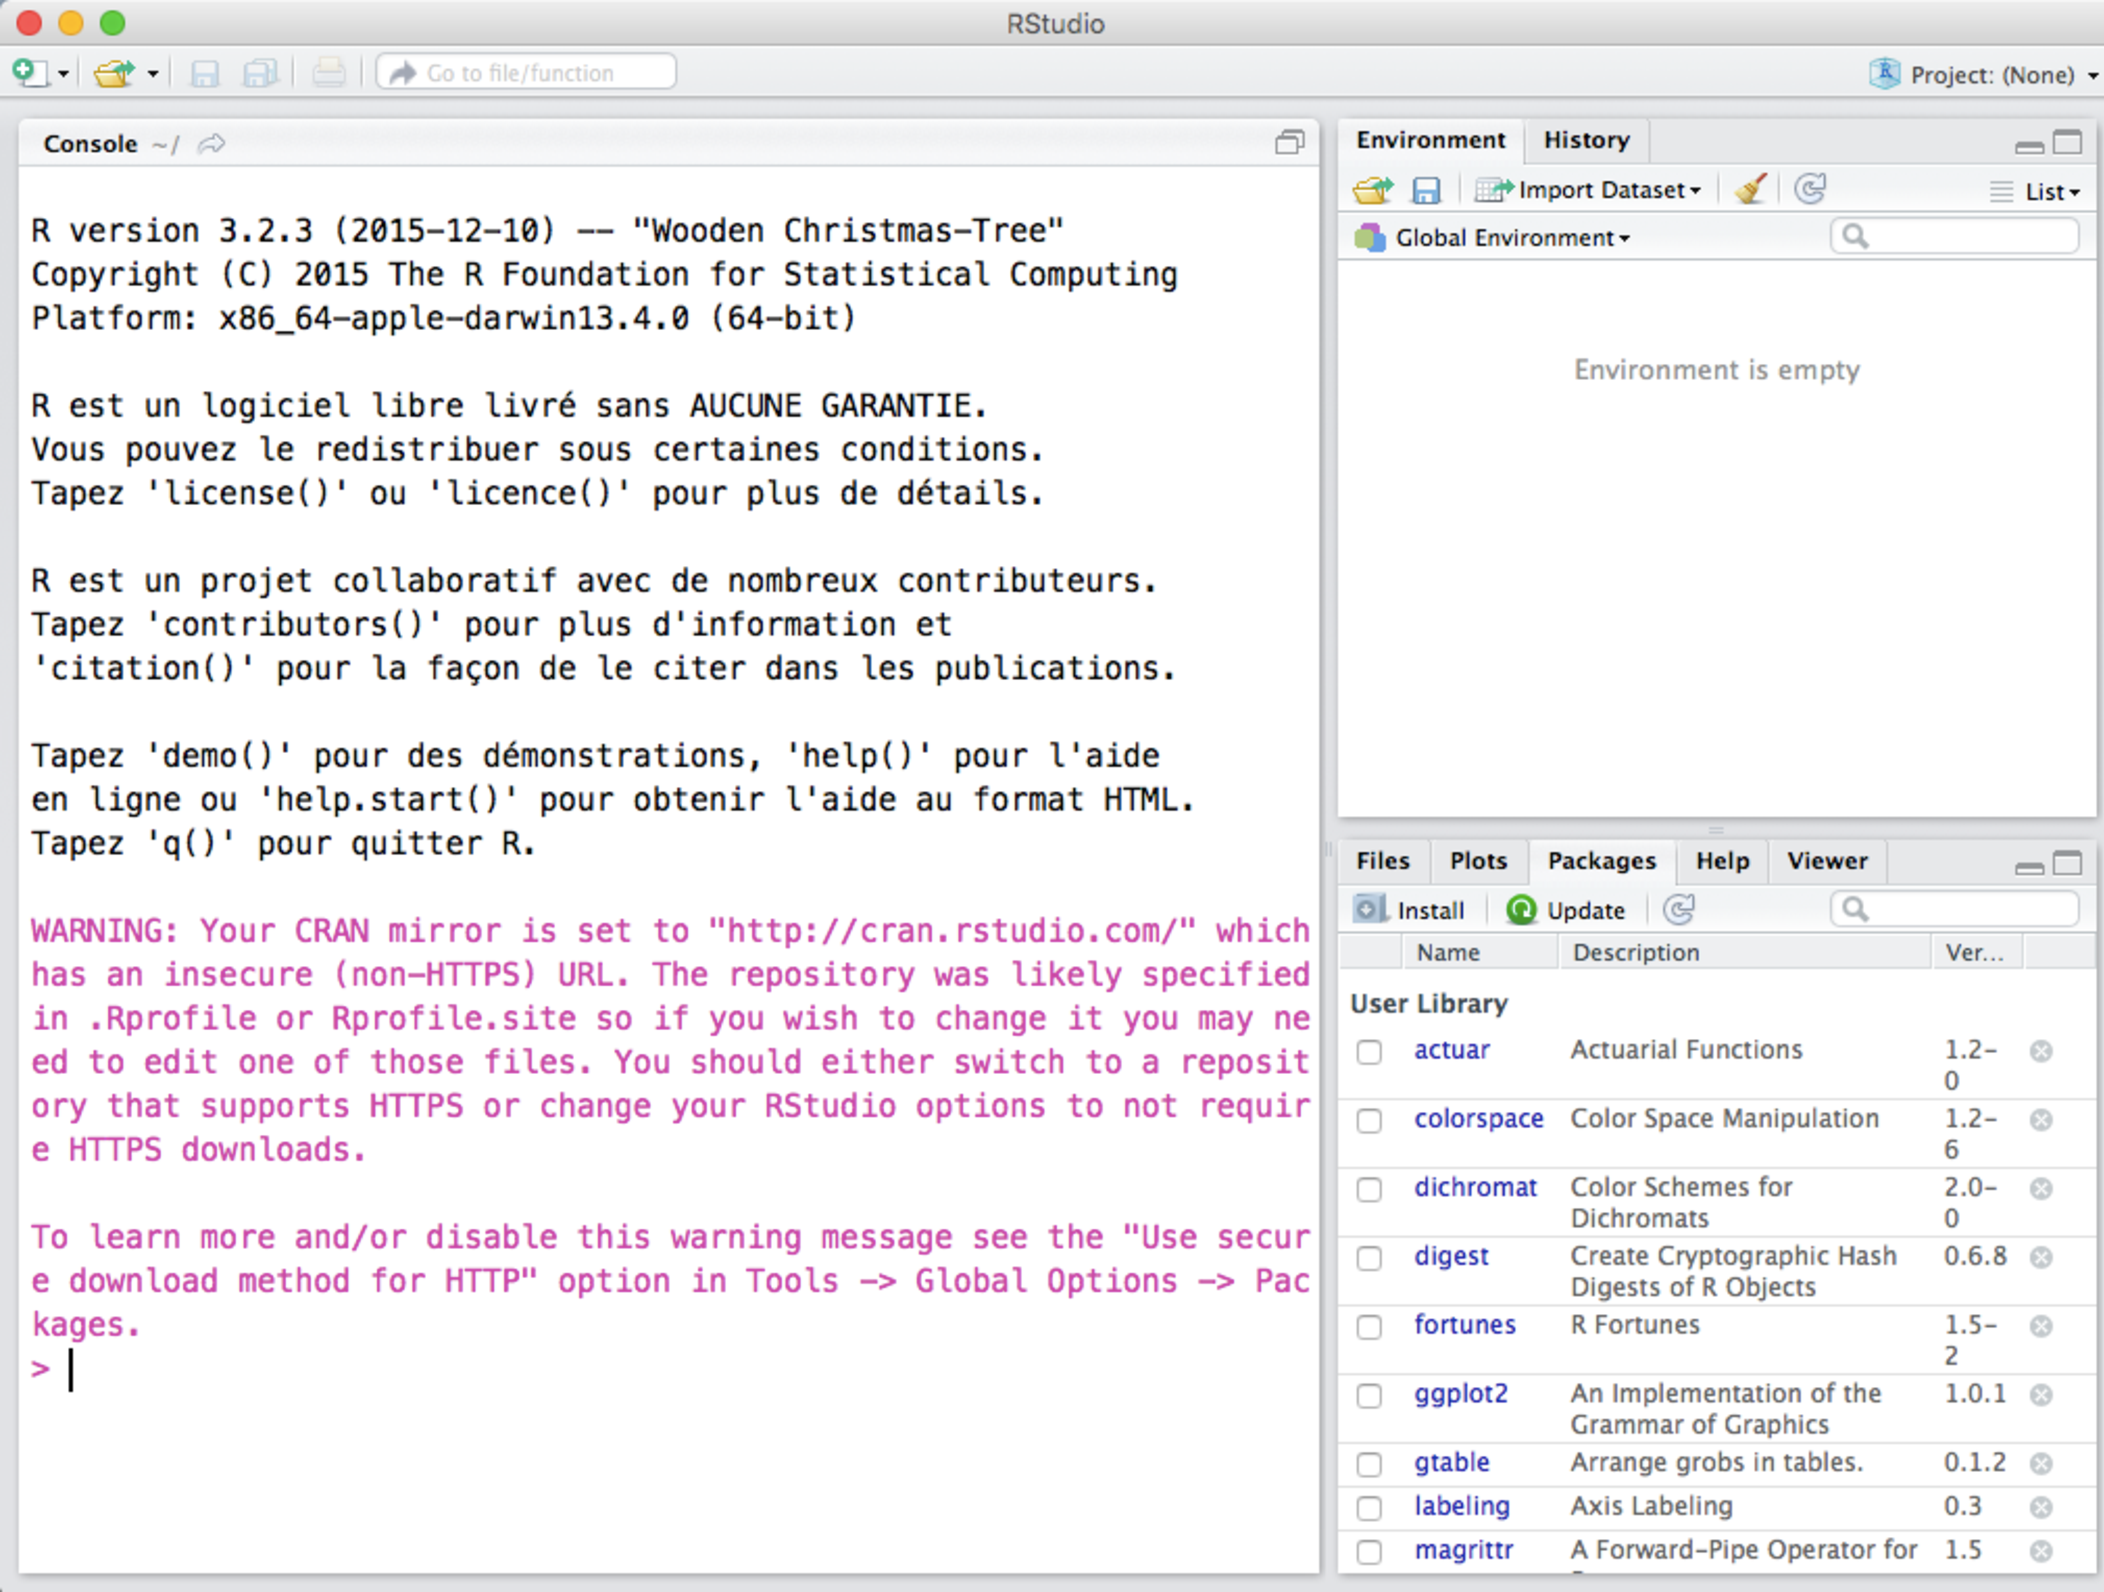
\includegraphics{rstudiowindow-screenshot}
  \vspace{0.5\TPVertModule}

  \begingroup
  \TPoptions{absolute=false}
  %% Identification de la console
  \begin{textblock}{0.5}(2.65,-0.62)
    \large\faLongArrowDown
  \end{textblock}
  \begin{textblock}{2}(2.2,-0.3)
    \footnotesize\sffamily Console R
  \end{textblock}

  %% Identification du navigateur d'environnement
  \begin{textblock}{1}(7.52,-3.65)
    \large\faLongArrowRight
  \end{textblock}
  \begin{textblock}{2.2}(7.95,-3.9)
    \footnotesize\sffamily\raggedright Navigateur d'environnement et d'historique
  \end{textblock}

  %% Identification de navigateur de fichiers
  \begin{textblock}{1}(7.52,-1.65)
    \large\faLongArrowRight
  \end{textblock}
  \begin{textblock}{2.2}(7.95,-1.9)
    \footnotesize\sffamily\raggedright Navigateur de fichiers, packages, graphiques, etc.
  \end{textblock}
  \endgroup
  \caption{Fenêtre de RStudio et trois de ses sous-fenêtres au
    lancement de l'application sous macOS. Sous Windows et Linux, la
    fenêtre comporte également une barre de menu.}
  \label{fig:rstudio:rstudiowindow}
\end{figure}

\begin{itemize}
\item Le navigateur d'environnement de travail est particulièrement
  utile pour voir le contenu, les attributs, le type et la taille de
  chaque objet sauvegardé dans la session R. Il permet également de
  visualiser le contenu des objets en cliquant sur leur nom ou sur
  l'icône de grille à droite de leur nom.
\item Il ne peut y avoir qu'un seul processus R (affiché dans la
  console) actif par fenêtre RStudio. Pour utiliser plusieurs
  processus R simultanément, il faut démarrer autant de copies de
  RStudio.
\item La position des sous-fenêtres dans la grille ne peut être
  modifiée. Par contre, chaque sous-fenêtre peut être redimensionnée.
\item On peut modifier la liste des onglets affichés dans les deux
  navigateurs dans les préférences de l'application; voir la
  \autoref{sec:rstudio:configuration}.
\end{itemize}


\section{Projets}
\index{RStudio!projets}
\label{sec:rstudio:projets}

Il est possible d'utiliser RStudio un peu comme un simple éditeur de
texte.
\begin{itemize}
\item On ouvre les fichiers de scripts un à un, soit à partir du menu
  \code{File|Open file...}, soit à partir de l'onglet \code{Files} du
  navigateur de fichiers.
\item Lorsque nécessaire, on change le répertoire de travail de R à
  partir du menu \code{Session}.
\end{itemize}

Pour faciliter l'organisation de son travail, l'ouverture des fichiers
de script et le lancement d'un processus R dans le bon répertoire de
travail, RStudio propose la notion de \emph{projet}.
\begin{itemize}
\item Un projet RStudio est associé à un répertoire de travail de R
  (\autoref{sec:presentation:workspace}).
\item On crée un nouveau projet à partir du menu \code{Project} à
  l'extrémité droite de la barre d'outils ou à partir du menu
  \code{File|New Project...} On a alors l'option de créer un nouveau
  dossier sur notre poste de travail ou de créer un projet à partir
  d'un dossier existant.
\item Lors de la création d'un projet, RStudio crée dans le dossier
  visé un fichier avec une extension \code{.Rproj} contenant diverses
  informations en lien avec le projet. De plus, le projet est
  immédiatement chargé dans RStudio.
\item L'ouverture d'un projet entraine: le lancement d'une session R
  dont le répertoire de travail est celui du projet; le
  chargement du fichier \code{.RData} (le cas échéant); l'ouverture de
  tous les fichiers de scripts qui étaient ouverts lors de la dernière
  séance de travail.
\item Chaque projet dispose de ses propres réglages. On accède à
  ceux-ci via la commande \code{Project Options...} du menu
  \code{Project} de la barre d'outils.
\end{itemize}

On trouvera plus d'information sur les projets dans l'aide en ligne
de RStudio.


\section{Commandes de base}
\label{sec:rstudio:commandes}

Comme l'interface de RStudio respecte les standards modernes, je ne
souligne ici que les commandes particulièrement utiles pour la
manipulation des fichiers de script. On accède rapidement à la liste
des commandes les plus utiles via le menu \code{Help} de
l'application.

Les raccourcis clavier sous, d'une part, Windows et Linux et sous,
d'autre part, macOS, différent légèrement. Je fournis ci-dessous
les deux jeux, séparés par le symbole $\bullet$.

\begin{ttscript}{Ctrl-Shift-S $\bullet$ \cmdkey\shiftkey S}
  \index{RStudio!symbole d'affectation}
\item[\code{Alt+-} $\bullet$ \code{\optkey\,-}] insérer le symbole
  d'affectation \verb*| <- | (pour les
  \capsule{https://youtu.be/aTyJfzE6pRw}{Mac avec un clavier
    canadien-français}, consulter l'encadré de la
  \autopageref{fig:rstudio:affectation})
\item[\code{Ctrl+Retour} $\bullet$ \code{\cmdkey\,\returnkey}]
  évaluer dans le processus R la ligne sous le curseur ou la région
  sélectionnée, puis déplacer le curseur à la prochaine expression
\item[\code{Ctrl+Shift+S} $\bullet$ \code{\shiftkey\,\cmdkey\,S}]
  évaluer le code du fichier courant en entier dans le processus R
\item[\code{Ctrl+Alt+B} $\bullet$ \code{\optkey\,\cmdkey\,B}]
  évaluer dans le processus R le code source du début du fichier
  jusqu'à la ligne sous le curseur
\item[\code{Ctrl+Alt+E} $\bullet$ \code{\optkey\,\cmdkey\,E}]
  évaluer dans le processus R le code source de la ligne sous le curseur
  jusqu'à la fin du fichier
\item[\code{Ctrl+Alt+F} $\bullet$ \code{\optkey\,\cmdkey\,F}]
  évaluer le code de la fonction courante dans le processus R
\end{ttscript}

À la console --- ou ligne de commande --- R, les raccourcis suivants
sont particulièrement utiles.
\begin{ttscript}{Ctrl-I $\bullet$ \cmdkey\,I}
\item[$\uparrow$ | $\downarrow$] expression
  précédente~|~suivante dans l'historique des commandes
\item[\code{Ctrl+}$\uparrow$ $\bullet$ \cmdkey\,$\uparrow$] afficher
  la fenêtre d'historique des commandes
\end{ttscript}

\begin{figure}[t]
  \begin{emphbox}{\mdseries Symbole d'affectation et
      Mac munis d'un clavier canadien-français}
    Le très pratique raccourci clavier {\optkey\,-} servant à insérer
    le symbole d'affectation ne fonctionne pas avec le clavier
    canadien-français sur les Mac. Cette combinaison de touches sert
    déjà à insérer le symbole \textbar. C'est en fait un doublon
    puisque, si l'on en croit le clavier, ce symbole est
    principalement lié à la
    touche {\optkey\,/}.

    Il est possible de régler le problème en redéfinissant le raccourci
    clavier associé au symbole d'affectation.

    \begin{enumerate}
    \item Ouvrir les préférences de RStudio (menu
      \code{RStudio|Preferences} ou {\cmdkey\,,}).
    \item Choisir la section \code{Code} dans la barre latérale de la
      fenêtre des options.
    \item Appuyer sur le bouton \code{Modify Keyboard Shortcuts\dots}.
    \item Une nouvelle fenêtre liste toutes les commandes disponibles
      et les raccourcis clavier associés. Dans le champ de recherche en
      haut, taper les lettres de «assignment» jusqu'à ce que la
      commande \code{Insert Assignment Operator} apparaisse.
    \item Cliquer sur la case du raccouci clavier (qui devrait être
      \code{Alt+-} par défaut) pour l'activer. Appuyer sur \optkey\,-
      pour utiliser cette combinaison de touches comme raccourci. Oui,
      on entre ce qui est apparemment la même combinaison de touches.
      Pour une raison quelconque, c'est «Alt+\bs» qui apparait alors
      comme raccourci.
    \item Fermer toutes les fenêtres de configuration.
    \end{enumerate}
  \end{emphbox}
  \label{fig:rstudio:affectation}
\end{figure}

\section{Anatomie d'une session de travail (bis)}
\label{sec:rstudio:session}

On reprend ici la description de %
%\capsule{http://youtu.be/xiNnHegDau8}{session de travail} %
la session de travail %
type présentée à la \autoref{sec:presentation:session}, mais en
expliquant comment compléter chaque étape dans RStudio. Sont
intercalés dans les instructions les raccourcis clavier des commandes
RStudio et les accès par les menus.

\begin{enumerate}
\item Lancer RStudio et ouvrir un nouveau fichier de script ou un
  fichier de script existant.
  \begin{trivlist}
  \item
    \makebox[0.38\linewidth][l]{%
      \colorbox{codebg}{\code{Ctrl+Shift+N} $\bullet$ \code{\shiftkey\,\cmdkey\,N}}}
    \hfill
    \makebox[0.58\linewidth][l]{%
      \colorbox{codebg}{\code{File|New File|R Script...}}}
  \item
    \makebox[0.38\linewidth][l]{%
      \colorbox{codebg}{\code{Ctrl+O} $\bullet$ \code{\cmdkey\,O}}}
    \hfill
    \makebox[0.58\linewidth][l]{%
      \colorbox{codebg}{\code{File|Open File...}}}
  \end{trivlist}
\item C'est une bonne pratique de faire du dossier où se trouve son ou
  ses fichiers de scripts le répertoire de travail de R.
  \begin{trivlist}
  \item
    \colorbox{codebg}{\code{Session|Set Working Directory|To Source File Location}}
  \end{trivlist}
\item Composer le code. Lors de cette étape de programmation, on se
  déplacera souvent du fichier de script à la console R afin
  d'essayer diverses expressions. On exécutera également des parties
  seulement du code se trouvant dans le fichier de script.
  \begin{trivlist}
  \item
    \makebox[0.38\linewidth][l]{%
      \colorbox{codebg}{\code{Ctrl+Retour} $\bullet$ \code{\cmdkey\,\returnkey}}}
    \hfill
    \makebox[0.58\linewidth][l]{%
      \colorbox{codebg}{\code{Code|Run Selected Line(s)}}}
  \item
    \makebox[0.38\linewidth][l]{%
      \colorbox{codebg}{\code{Ctrl+1} $\bullet$ \code{\cmdkey\,1}}}
    \hfill
    \makebox[0.58\linewidth][l]{%
      \colorbox{codebg}{\code{View|Move Focus to Source}}}
  \item
    \makebox[0.38\linewidth][l]{%
      \colorbox{codebg}{\code{Ctrl+2} $\bullet$ \code{\cmdkey\,2}}}
    \hfill
    \makebox[0.58\linewidth][l]{%
      \colorbox{codebg}{\code{View|Move Focus to Console}}}
  \end{trivlist}
\item Sauvegarder le fichier de script.
  \begin{trivlist}
  \item
    \makebox[0.38\linewidth][l]{%
      \colorbox{codebg}{\code{Ctrl+S} $\bullet$ \code{\cmdkey\,S}}}
    \hfill
    \makebox[0.58\linewidth][l]{%
      \colorbox{codebg}{\code{File|Save}}}
  \end{trivlist}
  (S'il s'agit d'un nouveau fichier, s'assurer de terminer son nom par
  \code{.R}.) Le nom du fichier dans l'onglet de la sous-fenêtre passe
  du rouge au noir.
\item Sauvegarder, si désiré, l'espace de travail de R avec
  \code{save.image()}\index{save.image@\code{save.image}}. Cela n'est
  habituellement pas nécessaire à moins que l'espace de travail ne
  contienne des objets importants ou longs à recréer.
  \begin{trivlist}
  \item
    \colorbox{codebg}{\code{Session|Save Workspace As...}}
  \end{trivlist}
\item Quitter RStudio de la manière usuelle. Par défaut, RStudio
  devrait demander si l'on souhaite sauvegarder l'espace de travail de
  R. Nous suggérons de ne pas le faire.

  La \autoref{sec:rstudio:configuration} explique comment configurer
  RStudio afin d'éviter de se faire poser la question à chaque
  fermeture de l'application.
\end{enumerate}


\section{Configuration de l'éditeur}
\index{RStudio!configuration}
\label{sec:rstudio:configuration}

Il est possible de configurer plusieurs facettes de RStudio à partir
d'une interface familière. On accède aux options de configuration par
le menu \code{Tools|Global Options...} sous Windows et Linux, et par le
menu standard \code{RStudio|Preferences} (\code{\cmdkey\,,})
sous macOS.

Nous recommandons de régler l'option
\begin{quote}
  \code{Save workspace to .RData on exit}
\end{quote}
à \code{Never} dans les options de configuration générales,
tel qu'illustré à la \autoref{fig:rstudio:rstudiopreferences}. Avec ce
réglage, l'espace de travail de R ne sera pas sauvegardé à la
fermeture de RStudio.

\begin{figure}
  \centering
  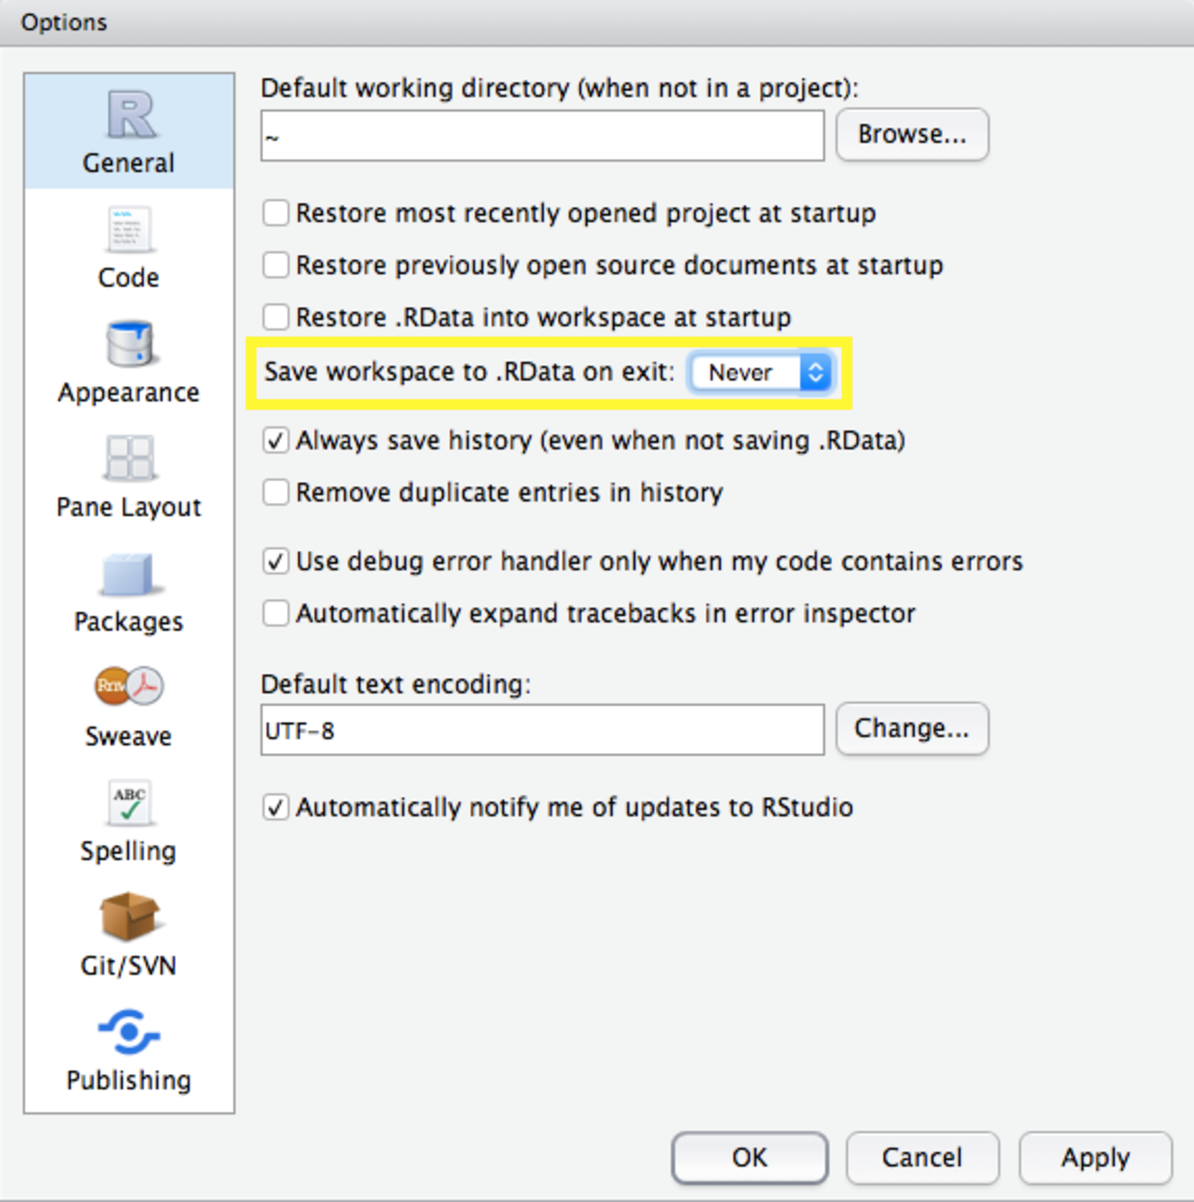
\includegraphics{rstudiopreferences-screenshot}
  \caption{Réglage suggéré de RStudio (encadré en jaune) faisant en
    sorte que l'espace de travail de R n'est jamais sauvegardé au
    moment de quitter l'application}
  \label{fig:rstudio:rstudiopreferences}
\end{figure}


\section{Aide et documentation}
\label{sec:rstudio:aide}

La documentation de RStudio se trouve entièrement en ligne. On y
accède par le menu \code{Help}. L'onglet \code{Help} du navigateur de
fichiers (sous-fenêtre en bas à droite) offre également une interface
unifiée pour accéder à l'aide de R et à celle de RStudio.

\index{RStudio|)}

%%% Local Variables:
%%% mode: latex
%%% TeX-engine: xetex
%%% TeX-master: "programmer-avec-r"
%%% coding: utf-8
%%% End:

\chapter{GNU Emacs et ESS: la base}
\index{Emacs|(}
\label{emacs+ess}

Emacs est l'Éditeur de texte des éditeurs de texte. À l'origine un
éditeur pour les programmeurs (avec des modes spéciaux pour une
multitude de langages différents), Emacs est devenu au fil du temps un
environnement logiciel en soi dans lequel on peut réaliser une foule
de tâches différentes: rédiger des documents {\LaTeX}, interagir avec R,
SAS ou un logiciel de base de données, consulter son courrier
électronique, gérer son calendrier ou même jouer à Tetris!

Cette annexe passe en revue les quelques commandes essentielles à
connaître pour commencer à travailler avec GNU Emacs et le mode ESS.
L'ouvrage de \cite{Cameron:Emacs:2004} constitue une excellente
référence pour l'apprentissage plus poussé de l'éditeur.

\setkeys{Gin}{width=370pt} % 1/2 la largeur de l'image insérée
\begin{figure}[t]
  \centering
  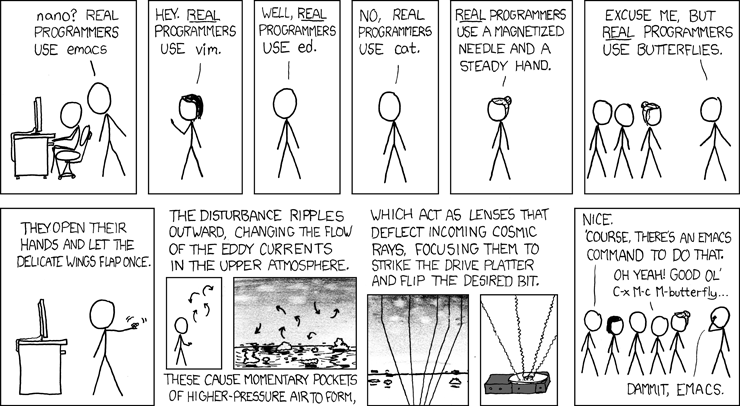
\includegraphics{emacs.png} \\
  \footnotesize\sffamily\flushleft\vspace{-\baselineskip}%
  Tiré de \href{http://xkcd.com/378/}{XKCD.com}. La commande \code{M-X
    butterfly} existe vraiment dans Emacs... en référence à cette
  bande dessinée!
\end{figure}
\setkeys{Gin}{width=0.8\textwidth}

\section{Mise en contexte}
\label{emacs+ess:contexte}

Emacs est le logiciel étendard du projet GNU («\emph{GNU is not
  Unix}»), dont le principal commanditaire est la \emph{Free Software
  Foundation} (FSF) à l'origine de tout le mouvement du logiciel
libre.
\begin{itemize}
\item Richard M.\ Stallman, président de la FSF et grand apôtre du
  libre, a écrit la première version de Emacs et il continue à ce jour
  à contribuer au projet.
\item Les origines de Emacs remontent au début des années 1980, une
  époque où les interfaces graphiques n'existaient pas, le parc
  informatique était beaucoup plus hétérogène qu'aujourd'hui (les
  claviers n'étaient pas les mêmes d'une marque d'ordinateur à une
  autre) et les modes de communication entre les ordinateurs
  demeuraient rudimentaires.
\item L'âge vénérable de Emacs transparaît à plusieurs endroits,
  notamment dans la terminologie inhabituelle, les raccourcis clavier
  non conformes aux standards d'aujourd'hui ou la manipulation des
  fenêtres qui ne se fait pas avec une souris.
\end{itemize}

Emacs s'adapte à différentes tâches par l'entremise de \emph{modes}
qui modifient son comportement ou lui ajoutent des fonctionnalités.
L'un de ces modes est ESS (\emph{Emacs Speaks Statistics}).
\begin{itemize}
\item ESS permet d'interagir avec des logiciels statistiques (en
  particulier R, S+ et SAS) directement depuis Emacs.
\item Quelques-uns des développeurs de ESS sont aussi des développeurs
  de R, d'où la grande compatibilité entre les deux logiciels.
\item Lorsque ESS est installé, le mode est activé automatiquement en
  ouvrant dans Emacs un fichier dont le nom se termine par l'extension
  \code{.R}.
\end{itemize}


\section{Installation}
\label{emacs+ess:installation}

GNU Emacs et le mode ESS sont normalement livrés d'office avec toutes
les distributions Linux. Pour les environnements Windows et OS~X,
le plus simple consiste à installer les distributions préparées par le
présent auteur. Consulter le site
\begin{quote}
  \url{http://vgoulet.act.ulaval.ca/emacs/}
\end{quote}


\section{Description sommaire}
\label{emacs+ess:description}

Au lancement, Emacs affiche un écran d'information contenant des liens
vers différentes ressources. Cet écran disparaît dès que l'on appuie
sur une touche. La fenêtre Emacs se divise en quatre zone principales
(voir la \autoref{fig:ess:emacswindow}):
\begin{enumerate}
\item tout au haut de la fenêtre (ou de l'écran sous OS~X), on trouve
  l'habituelle barre de menu dont le contenu change selon le mode dans
  lequel se trouve Emacs;
\item l'essentiel de la fenêtre sert à afficher un \emph{buffer}, soit
  le contenu d'un fichier ouvert ou l'invite de commande d'un
  programme externe;
\item la ligne de mode est le séparateur horizontal contenant diverses
  informations sur le fichier ouvert et l'état de Emacs;
\item le \emph{minibuffer} est la région au bas de la fenêtre où l'on
  entre des commandes et reçoit de l'information de Emacs.
\end{enumerate}
Il est possible de séparer la fenêtre Emacs en sous-fenêtres pour
afficher plusieurs \emph{buffers} à la fois. Il y a alors une ligne de
mode pour chaque \emph{buffer}.

\begin{figure}[t]
  %% Capture d'écran
  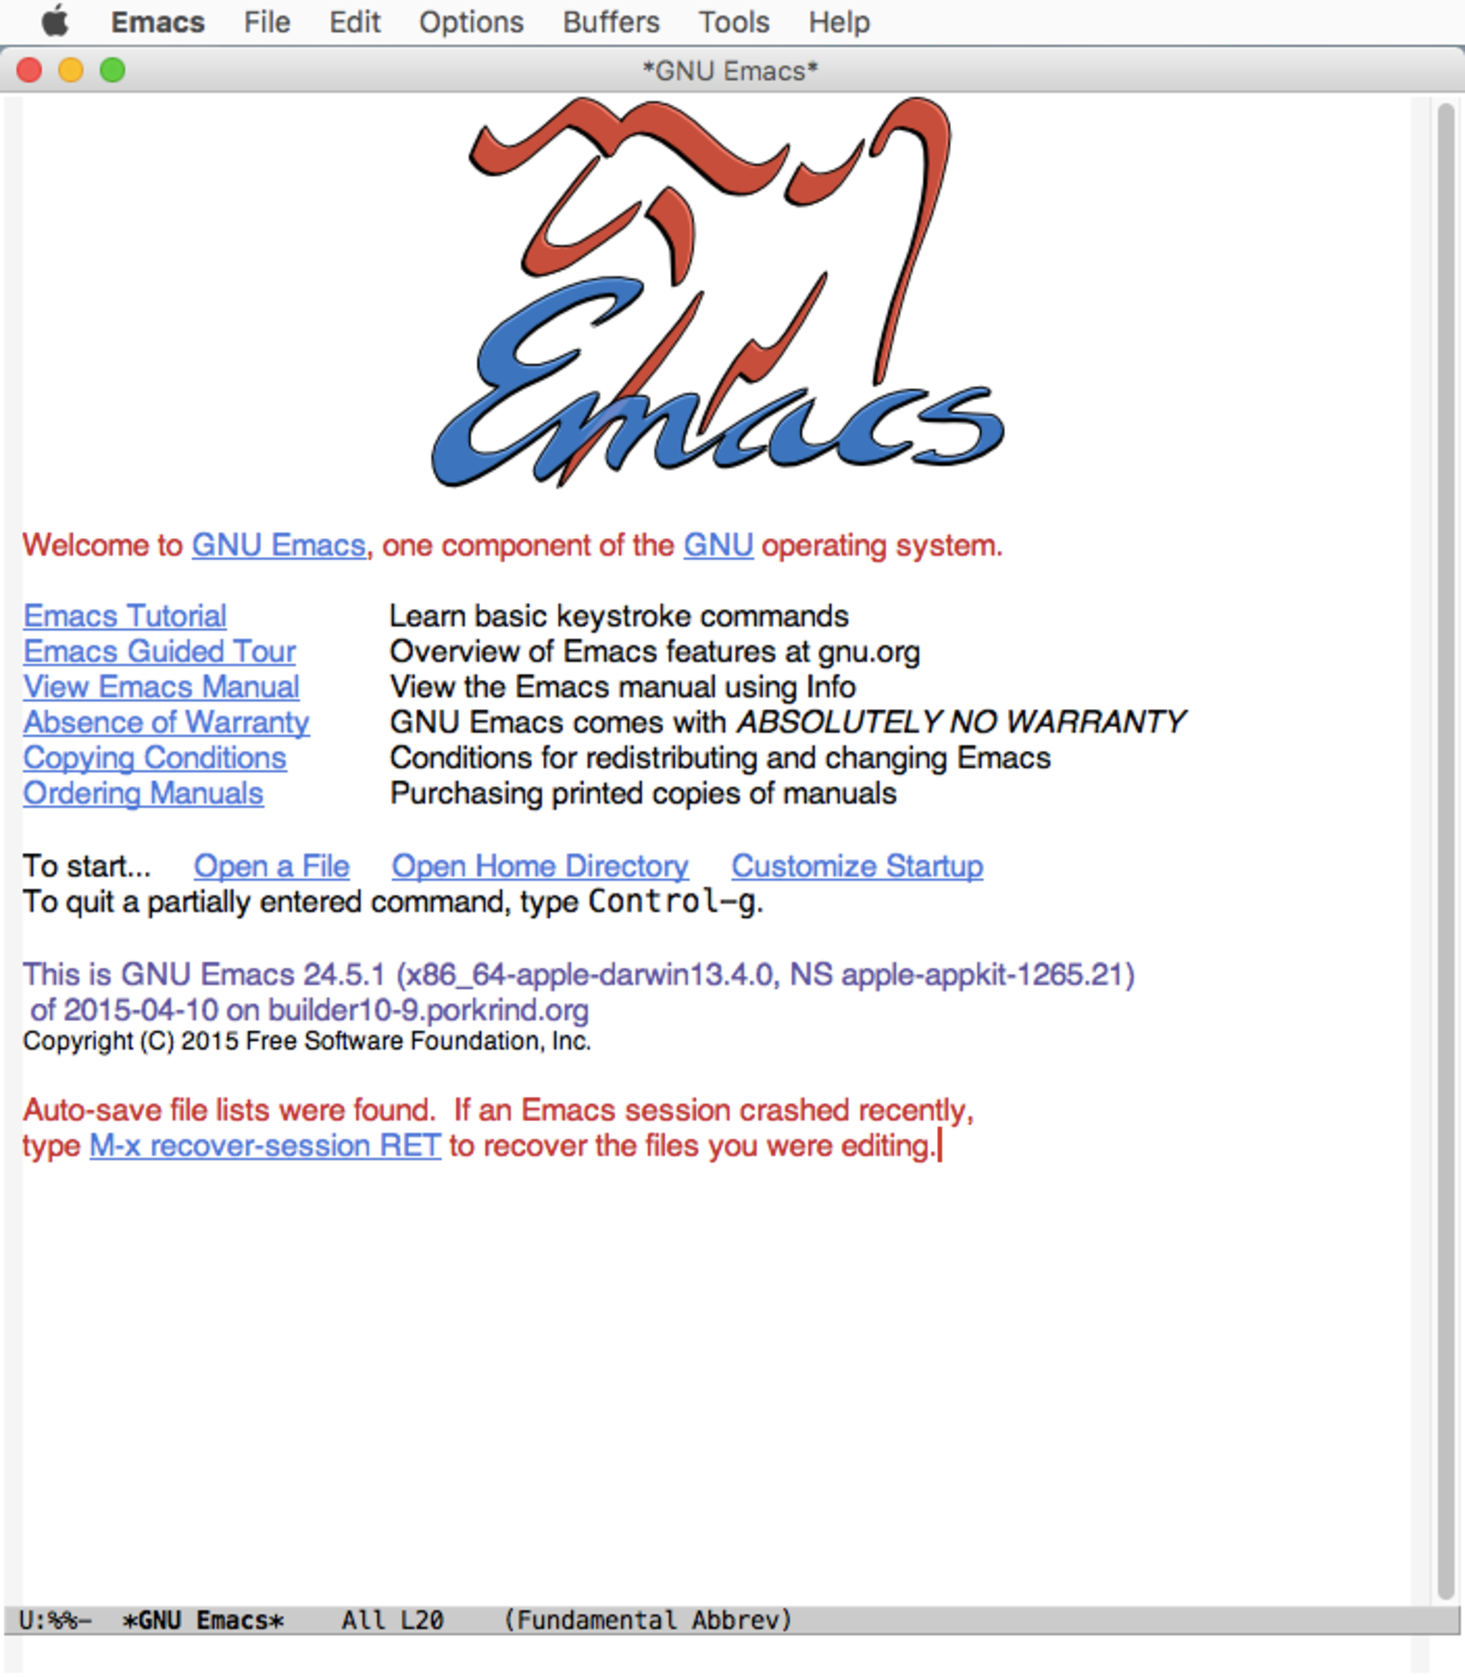
\includegraphics{emacswindow-screenshot}

  %% Identification de la barre de menu
  \begin{textblock}{0.35}(7.38,-6.58)
    \Large\faLongArrowRight
  \end{textblock}
  \begin{textblock}{1.75}(7.88,-6.59)
    \footnotesize\sffamily Barre de menu
  \end{textblock}

  %% Identification du buffer
  \begin{textblock}{0.35}(7.38,-3.38)
    \Large\faLongArrowRight
  \end{textblock}
  \begin{textblock}{1.75}(7.88,-3.39)
    \footnotesize\sffamily \emph{Buffer}
  \end{textblock}

  %% Identification de la mode line
  \begin{textblock}{0.35}(7.38,-0.28)
    \Large\faLongArrowRight
  \end{textblock}
  \begin{textblock}{1.75}(7.88,-0.29)
    \footnotesize\sffamily Ligne de mode
  \end{textblock}

  %% Identification du minibuffer
  \begin{textblock}{0.35}(7.38,-0.08)
    \Large\faLongArrowRight
  \end{textblock}
  \begin{textblock}{1.75}(7.88,-0.09)
    \footnotesize\sffamily \emph{Minibuffer}
  \end{textblock}
  \caption{Fenêtre GNU~Emacs et ses différentes parties au lancement
    de l'application sous OS~X. Sous Windows et Linux, la barre de
    menu se trouve à l'intérieur de la fenêtre.}
  \label{fig:ess:emacswindow}
\end{figure}


\section{\emph{Emacs-ismes} et \emph{Unix-ismes}}
\label{emacs+ess:ismes}

Emacs possède sa propre terminologie qu'il vaut mieux connaître
lorsque l'on consulte la documentation. De plus, l'éditeur utilise des
conventions du monde Unix qui sont moins usitées sur les plateformes
Windows et OS~X.

\begin{itemize}
\item Dans les définitions de raccourcis claviers:
  \begin{itemize}
  \item \code{C} est la touche \code{Contrôle} (\ctlkey);
  \item \code{M} est la touche \code{Meta}, qui correspond à la touche
    \code{Alt} de gauche sur un PC ou la touche \code{Option}
    (\optkey) sur un Mac (toutefois, voir l'encadré à la
    \autopageref{fig:ess:meta});
  \item \code{ESC} est la touche \code{Échap} (\esckey) et
    est équivalente à \code{Meta};
  \item \code{SPC} est la barre d'espacement;
  \item \code{DEL} est la touche \code{Retour arrière} (\delkey) ---
    \emph{et non la touche} \code{Supprimer}.
  \item \code{RET} est la touche \code{Entrée} (\returnkey);
  \end{itemize}
\item Toutes les fonctionnalités de Emacs correspondent à une commande
  pouvant être tapée dans le \emph{minibuffer}. \code{M-x} démarre
  l'invite de commande.
\item Le caractère \,\verb=~=\, représente le dossier vers lequel
  pointe la variable d'environnement \code{\$HOME} (Linux, OS~X) ou
  \code{\%HOME\%} (Windows). C'est le dossier par défaut de Emacs.
\item La barre oblique (\code{/}) est utilisée pour séparer les
  dossiers dans les chemins d'accès aux fichiers, même sous Windows.
\item En général, il est possible d'appuyer sur \code{TAB} dans le
  \emph{minibuffer} pour compléter les noms de fichiers ou de
  commandes.
\end{itemize}

\begin{figure}[t]
  \begin{osx}
    Par défaut sous OS~X, la touche \code{Meta} est assignée à
    \code{Option} (\optkey). Sur les claviers français, cela empêche
    d'accéder à certains caractères spéciaux tels que [, ], \{ ou \}.

    Une solution à cette fâcheuse situation consiste à assigner
    la touche \code{Meta} à \code{Commande} (\cmdkey). Cela bloque
    alors l'accès à certains raccourcis Mac, mais la situation est
    moins critique ainsi.

    Pour assigner la touche \code{Meta} à \code{Commande} (\cmdkey) et
    laisser la touche \code{Option} (\optkey) jouer son rôle usuel, il
    suffit d'insérer les lignes suivantes dans son fichier de
    configuration \code{.emacs} (voir la
    \autoref{emacs+ess:configuration}):
\begin{verbatim}
;;; ====================================
;;;  Assigner la touche Meta à Commande
;;;  et laisser Option être Option
;;; ====================================
(setq-default ns-command-modifier 'meta)
(setq-default ns-option-modifier 'none)
\end{verbatim}
  \end{osx}
  \label{fig:ess:meta}
\end{figure}



\section{Commandes de base}
\label{emacs+ess:commandes}

Emacs comporte une pléthore de commandes, il serait donc futile de
tenter d'en faire une liste exhaustive ici. Nous nous contenterons de
mentionner les commandes les plus importantes regroupées par tâche.

% Pour débuter, il est utile de suivre le Tour guidé de Emacs\footnote{%
%   \url{http://www.gnu.org/software/emacs/tour/} ou cliquer sur le lien
%   dans l'écran d'accueil.} %
% et de lire le tutoriel de Emacs, que l'on démarre avec \code{C-h t}.

\subsection{Les essentielles}
\label{emacs+ess:commandes:essentielles}

\begin{ttscript}{M-x}
\item[\code{M-x}] démarrer l'invite de commande
\item[\code{C-g}] bouton de panique: annuler, quitter! Presser plus
  d'une fois au besoin.
\end{ttscript}

\subsection{Manipulation de fichiers}
\label{emacs+ess:commandes:fichiers}

Entre parenthèses, le nom de la commande Emacs correspondante. On peut
entrer cette commande dans le \emph{minibuffer} au lieu d'utiliser le
raccourci clavier.

\begin{important}
  On remarquera qu'il n'existe pas de commande «nouveau fichier» dans
  Emacs. Pour créer un nouveau fichier, il suffit d'ouvrir un fichier
  n'existant pas.\index{Emacs!nouveau fichier}
\end{important}

\begin{ttscript}{C-x C-w}
  \raggedright
\item[\code{C-x C-f}] ouvrir un fichier (\code{find-file})
\item[\code{C-x C-s}] sauvegarder
  (\code{save-buffer})\index{Emacs!sauvegarder}
\item[\code{C-x C-w}] sauvegarder sous
  (\code{write-file})\index{Emacs!sauvegarder sous}
\item[\code{C-x k}] fermer un fichier (\code{kill-buffer})
  \\[\baselineskip]
\item[\code{C-\_}] annuler (pratiquement illimité); aussi
  \code{C-x u} (\code{undo})
  \\[\baselineskip]
\item[\code{C-s}] recherche incrémentale avant
  (\code{isearch-forward})
\item[\code{C-r}] Recherche incrémentale arrière
  (\code{isearch-backward})
\item[\code{M-\%}] rechercher et remplacer
  (\code{query-replace})\index{Emacs!rechercher et remplacer}
\end{ttscript}


\subsection{Déplacements simples du curseur}
\index{Emacs!déplacement du curseur}
\label{emacs+ess:commandes:deplacement}

\begin{ttscript}{C-DEL | C-w}
  \raggedright
\item[\code{C-b} | \code{C-f}] déplacer d'un caractère vers l'arrière~|~l'avant
  (\code{backward-char} | \code{forward-char})
\item[\code{C-a} | \code{C-e}] aller au début~|~fin de la ligne
  (\code{move-beginning-of-line} | \code{move-end-of-line})
\item[\code{C-p} | \code{C-n}] aller à la ligne précédente~|~suivante
  (\code{previous-line} | \code{next-line})
\item[\code{M-<} | \code{M->}] aller au début~|~fin du fichier
  (\code{beginning-of-buffer} | \code{end-of-buffer}) \\[\baselineskip]
\item[\code{DEL} | \code{C-d}] effacer le caractère à
  gauche~|~droite du curseur (\code{delete-backward-char} | \code{delete-char})
\item[\code{M-DEL} | \code{M-d}] effacer le mot à gauche~|~droite
  du curseur (\code{backward-kill-word} | \code{kill-word})
\item[\code{C-k}] supprimer jusqu'à la fin de la ligne (\code{kill-line})
\end{ttscript}

\begin{figure}[ht]
  \begin{osx}
    Plusieurs des raccourcis clavier de Emacs composés avec la touche
    \code{Contrôle} (\ctlkey) sont valides sous OS~X. Par exemple,
    \ctlkey\,\code{A} et \ctlkey\,\code{E} déplacent le curseur au
    début et à la fin de la ligne dans les champs texte.
  \end{osx}
\end{figure}


\subsection{Sélection de texte, copier, coller, couper}
\index{Emacs!sélection}
\label{emacs+ess:commandes:selection}

\begin{ttscript}{C-x C-w}
  \raggedright
\item[\code{C-SPC}] débute la sélection (\code{set-mark-command})
\item[\code{C-w}] couper la sélection (\code{kill-region})
\item[\code{M-w}] copier la sélection (\code{kill-ring-save})
\item[\code{C-y}] coller (\code{yank})
\item[\code{M-y}] remplacer le dernier texte collé par la
  sélection précédente (\code{yank-pop})
\end{ttscript}

\begin{itemize}
\item Il est possible d'utiliser les raccourcis clavier usuels de
  Windows (\code{C-c}, \code{C-x}, \code{C-v}) et OS~X
  (\cmdkey\,\code{C}, \cmdkey\,\code{X}, \cmdkey\,\code{V}) en
  activant le mode CUA dans le menu \code{Options}.
\item On peut copier-coller directement avec la souris dans Windows en
  sélectionnant du texte puis en appuyant sur le bouton central (ou la
  molette) à l'endroit souhaité pour y copier le texte.
\end{itemize}


\subsection{Manipulation de fenêtres}
\label{emacs+ess:commandes:fenetres}

\begin{ttscript}{C-x C-w}
\item[\code{C-x b}] changer de \emph{buffer}
  (\code{switch-buffer})
\item[\code{C-x 2}] séparer l'écran en deux fenêtres
  (\code{split-window-vertically})
\item[\code{C-x 1}] conserver uniquement la fenêtre courante
  (\code{delete-other-windows})
\item[\code{C-x 0}] fermer la fenêtre courante
  (\code{delete-window})
\item[\code{C-x o}] aller vers une autre fenêtre lorsqu'il y en a
  plus d'une (\code{other-window})
\end{ttscript}

\subsection{Manipulation de fichiers de script dans le mode ESS}
\index{Emacs!mode ESS|(}
\label{emacs+ess:commandes:script}

Le mode ESS dispose de fonctions «intelligentes» qui facilitent
grandement la manipulation des fichiers de script. Les deux
principales commandes à connaître sont les suivantes:
\begin{ttscript}{C-x C-w}
  \raggedright
\item[\code{C-RET}] évaluer dans le processus R la ligne sous le
  curseur ou la région sélectionnée, puis déplacer le curseur à la
  prochaine expression (\code{ess-eval-region-or-line-and-step})
\item[\code{C-c C-c}] évaluer dans le processus R la région
  sélectionnée, la fonction ou le paragraphe (tout bloc entre deux
  lignes blanches) dans lequel se trouve le curseur, puis déplacer le
  curseur à la prochaine expression
  (\code{ess-eval-region-or-function-or-paragraph-and-step})
\end{ttscript}
Les quelques autres fonctions utiles sont:
\begin{ttscript}{C-x C-w}
  \raggedright
\item[\code{C-c C-z}] déplacer le curseur vers le processus R
  (\code{ess-switch-to-inferior-or-script-buffer})
\item[\code{C-c C-f}] évaluer le code de la fonction courante dans
  le processus R (\code{ess-eval-function})
\item[\code{C-c C-l}] évaluer le code du fichier courant en entier dans
  le processus R (\code{ess-load-file})
\item[\code{C-c C-v}] aide sur une commande R
  (\code{ess-display-help-on-object})
\end{ttscript}

\subsection{Interaction avec l'invite de commande R}
\label{emacs+ess:commandes:invite}

\begin{ttscript}{M-p |M-n}
  \raggedright
\item[\code{M-p} | \code{M-n}] commande précédente~|~suivante
  dans l'historique (\code{previous-matching-history-from-input},
  \code{next-matching-history-from-input})
\item[\code{C-c C-z}] déplacer le curseur vers le fichier de script
  courant (\code{ess-switch-to-inferior-or-script-buffer})
\item[\code{M-h}] sélectionner le résultat de la dernière commande
  (\code{mark-paragraph})
\item[\code{C-c C-o}] effacer le résultat de la dernière commande
  (\code{comint-delete-output})
\item[\code{C-c C-v}] aide sur une commande R
  (\code{ess-display-help-on-object})
\item[\code{C-c C-q}] terminer le processus R (\code{ess-quit})
\end{ttscript}

\subsection{Consultation des rubriques d'aide de R}
\label{emacs+ess:commandes:aide}

\begin{ttscript}{m, m}
  \raggedright
\item[\code{p} | \code{n}] aller à la section précédente~|~suivante de
  la rubrique (\code{ess-skip-to-previous-section} |
  \code{ess-skip-to-next-section})
\item[\code{s a}] aller à la section de la liste des arguments \emph{(Arguments)}
\item[\code{s D}] aller à la section des détails sur la fonction \emph{(Details)}
\item[\code{s v}] aller à la section sur la valeur retournée par la
  fonction \emph{(Value)}
\item[\code{s s}] aller à la section des fonctions apparentée \emph{(See Also)}
\item[\code{s e}] aller à la section des exemples \emph{(Examples)}
\item[\code{l}] évaluer la ligne sous le curseur; pratique pour
  exécuter les exemples (\code{ess-eval-line-and-step})
\item[\code{r}] évaluer la région sélectionnée (\code{ess-eval-region})
\item[\code{h}] ouvrir une nouvelle rubrique d'aide, par défaut pour le
  mot se trouvant sous le curseur (\code{ess-display-help-on-object})
\item[\code{q}] retourner au processus ESS en laissant la rubrique
  d'aide visible (\code{ess-switch-to-end-of-ESS})
\item[\code{x}] fermer la rubrique d'aide et retourner au processus ESS
  (\code{ess-kill-buffer-and-go})
\end{ttscript}



\section{Anatomie d'une session de travail (bis)}
\label{emacs+ess:session}

On reprend ici les étapes d'une \capsule{http://youtu.be/xiNnHegDau8}{session de
  travail} type présentées à la \autoref{presentation:session}, mais
en expliquant comment compléter chacune dans Emacs avec le mode ESS.

\begin{enumerate}
\item Lancer Emacs et ouvrir un fichier de script avec
  \begin{quote}
    \code{C-x C-f}
  \end{quote}
  ou avec le menu
  \begin{quote}
    \code{File|Open File...}
  \end{quote}
  En spécifiant un nom de fichier qui n'existe pas déjà, on se trouve
  à créer un nouveau fichier de script. S'assurer de terminer le nom
  du nouveau fichier par \code{.R} pour que Emacs reconnaisse
  automatiquement qu'il s'agit d'un fichier de script R.
\item Démarrer un processus R à l'intérieur même de Emacs avec
  \begin{quote}
    \code{M-x R }\returnkey
  \end{quote}
  Emacs demandera alors de spécifier de répertoire de travail
  (\emph{starting data directory}). Accepter la valeur par défaut, par
  exemple
  \begin{quote}
    \verb=~/ =\returnkey
  \end{quote}
  ou indiquer un autre dossier. Un éventuel message de Emacs à l'effet
  que le fichier \code{.Rhistory} n'a pas été trouvé est sans
  conséquence et peut être ignoré.
\item Composer le code. Lors de cette étape, on se déplacera souvent
  du fichier de script à la ligne de commande afin d'essayer diverses
  expressions. On exécutera également des parties seulement du code se
  trouvant dans le fichier de script. Les commandes les plus utilisées
  sont alors:
  \begin{quote}
    \begin{ttscript}{C-c C-z}
      \renewcommand{\makelabel}[1]{#1\hfill}
    \item[\code{C-RET}] pour exécuter une ligne du fichier de script ou la
      région sélectionnée;
    \item[\code{C-c C-c}] pour exécuter un paragraphe du fichier de
      script;
    \item[\code{C-c C-z}] pour se déplacer entre le fichier de script et
      la ligne de commande R.
    \end{ttscript}
  \end{quote}
\item Sauvegarder le fichier de script:
  \begin{quote}
    \code{C-x C-s}
  \end{quote}
  Les quatrième et cinquième caractères de la ligne de mode changent
  de \,\verb|**|\, à \,\verb|--|.
\item Sauvegarder si désiré l'espace de travail de R avec
  \code{save.image()}\indexfonction{save.image}. Cela n'est
  habituellement pas nécessaire à moins que l'espace de travail ne
  contienne des objets importants ou longs à recréer.
\item Quitter le processus R avec
  \begin{quote}
    \code{C-c C-q}
  \end{quote}
  Cette commande ESS se chargera de fermer tous les fichiers associés
  au processus R. On peut ensuite quitter Emacs en fermant
  l'application de la manière usuelle.
\end{enumerate}
\index{Emacs!mode ESS|)}



\section{Configuration de l'éditeur}
\label{emacs+ess:configuration}

Une des grandes forces de Emacs est qu'à peu près chacune de ses
facettes est configurable: couleurs, polices de caractère, raccourcis
clavier, etc.

\begin{itemize}
\item La configuration de Emacs se fait par le biais de commandes
  réunies dans un \capsule{http://youtu.be/IsyQn7d2Ao0}{fichier de
    configuration} nommé \code{.emacs} (le point est important!) que
  Emacs lit au démarrage.
\item Le fichier \code{.emacs} doit se trouver dans le dossier
  \,\verb=~/=, c'est-à-dire dans le dossier de départ de l'utilisateur
  sous Linux et OS~X, et dans le dossier référencé par la variable
  d'environnement \code{\%HOME\%} sous Windows.
\end{itemize}


\section{Aide et documentation}
\label{emacs+ess:aide}

Emacs possède son propre système d'aide très exhaustif, mais dont la
navigation est peu intuitive selon les standards d'aujourd'hui.
Consulter le menu \code{Help}.

Autrement, on trouvera les manuels de Emacs et de ESS en divers
formats dans les sites respectifs des deux projets:
\begin{quote}
  \url{http://www.gnu.org/software/emacs} \\
  \url{http://ess.r-project.org}
\end{quote}

Enfin, si le désespoir vous prend au cours d'une séance de codage
intensive, vous pouvez toujours consulter le psychothérapeute Emacs.
On le trouve, bien entendu, dans le menu \code{Help}!

\index{Emacs|)}

%%% Local Variables:
%%% mode: latex
%%% TeX-master: "introduction_programmation_r"
%%% coding: utf-8
%%% End:

% \chapter{Installation de packages dans R}
\index{package!installation|(}
\label{packages}

Un package R est un ensemble cohérent de fonctions, de jeux de données
et de documentation permettant de compléter les fonctionnalités du
système de base ou d'en ajouter de nouvelles. Les packages sont normalement
installés depuis le site \emph{Comprehensive R Archive Network} (CRAN;
\url{http://cran.r-project.org}).

Cette annexe explique comment configurer R pour faciliter l'%
\capsule{https://youtu.be/DL48oi2RKjM}{installation et l'administration
  de packages} %
externes.

Les instructions ci-dessous se basent sur la création d'une
bibliothèque personnelle\index{package!bibliothèque personnelle} où
seront installés les packages R téléchargés de CRAN. Il est fortement
recommandé de créer une telle bibliothèque. Cela permet d'éviter les
éventuels problèmes d'accès en écriture dans la bibliothèque
principale et de conserver les packages intacts lors des mises à jour
de R. On montre également comment spécifier le site miroir de CRAN
pour éviter d'avoir à le répéter à chaque installation de package.
\begin{enumerate}
\item Identifier le dossier de départ de l'utilisateur. En cas
  d'incertitude, examiner la valeur de la variable d'environnement
  \code{HOME}\footnote{%
    Pour les utilisateurs de GNU~Emacs sous Windows, la variable est
    créée par l'assistant d'installation de Emacs lorsqu'elle n'existe
    pas déjà.}, %
  depuis R avec la commande
\begin{Schunk}
\begin{Sinput}
> Sys.getenv("HOME")
\end{Sinput}
\end{Schunk}
  ou, pour les utilisateurs de Emacs, directement depuis l'éditeur avec
\begin{verbatim}
M-x getenv RET HOME RET
\end{verbatim}
  Nous référerons à ce dossier par le symbole \verb=~=.
\item Créer un dossier qui servira de bibliothèque de packages
  personnelle. Dans la suite, nous utiliserons \verb=~/R/library=.
\item La configuration de R se fait à l'aide simples fichiers texte,
  comme pour GNU~Emacs; voir la \autoref{emacs+ess:configuration}.
  Dans un fichier nommé \verb=~/.Renviron= (donc situé dans le dossier
  de départ), enregistrer la ligne suivante:
\begin{verbatim}
R_LIBS_USER="~/R/library"
\end{verbatim}
  Au besoin, remplacer le chemin \verb=~/R/library= par celui du
  dossier créé à l'étape précédente. Utiliser la barre oblique avant
  (\code{/}) dans le chemin pour séparer les dossiers.
  \begin{osx}
    Sous OS~X, ajouter dans le fichier \verb=~/.Renviron= la ligne
    suivante:
\begin{verbatim}
R_INTERACTIVE_DEVICE=quartz
\end{verbatim}
    Ainsi, R utilisera toujours l'interface Quartz\index{Quartz} native
    de OS~X pour afficher les graphiques.
  \end{osx}
\item Dans un fichier nommé \verb=~/.Rprofile=, enregistrer l'option
  suivante:
\begin{verbatim}
options(repos = "http://cran.ca.r-project.org")
\end{verbatim}
  Si désiré, remplacer la valeur de l'option \code{repos} par l'URL
  d'un autre site miroir de CRAN.

  Les utilisateurs de GNU~Emacs voudront ajouter une option pour
  éviter que R ait recours aux menus graphiques Tcl/Tk. Le code à
  entrer dans le fichier \verb=~/.Rprofile= sera plutôt
\begin{verbatim}
options(repos = "http://cran.ca.r-project.org",
        menu.graphics = FALSE)
\end{verbatim}
\end{enumerate}
Consulter la rubriques d'aide de \code{Startup} pour les détails sur
la syntaxe et l'emplacement des fichiers de configuration, celles de
\code{library} et \code{.libPaths} pour la gestion des bibliothèques
et celle de \code{options} pour les différentes options reconnues par
R.

Après un redémarrage de R, la bibliothèque personnelle aura préséance
sur la bibliothèque principale et il ne sera plus nécessaire de
préciser le site miroir de CRAN lors de l'installation de packages.
Ainsi, la simple commande
\begin{Schunk}
\begin{Sinput}
> install.packages("actuar")
\end{Sinput}
\end{Schunk}
téléchargera le package de fonctions actuarielles \textbf{actuar}
depuis le miroir canadien de CRAN et l'installera dans le dossier
\verb=~/R/library=. Pour charger le package en mémoire, on fera
\begin{Schunk}
\begin{Sinput}
> library("actuar")
\end{Sinput}
\end{Schunk}

On peut arriver au même résultat sans utiliser les fichiers de
configuration \code{.Renviron} et \code{.Rprofile}. Il faut cependant
recourir aux arguments \code{lib} et \code{repos} de la fonction
\code{install.packages} et à l'argument \code{lib.loc} de la fonction
\code{library}. Consulter les rubriques d'aide de ces deux fonctions
pour de plus amples informations.

\index{package!installation|)}

%%% Local Variables:
%%% mode: latex
%%% TeX-master: "introduction_programmation_r"
%%% coding: utf-8
%%% End:

\chapter{Réponses des exercices}
\label{chap:reponses}

\begingroup

%% Environnement Schunk simplifié pour l'affichage des réponses
\renewenvironment{Schunk}{%
  \setlength{\topsep}{0pt}
  \colorlet{shadecolor}{codebg}
  \begin{snugshade*}}%
  {\end{snugshade*}}

\input{solutions-informatique}
\input{solutions-bases}
\input{solutions-implementation}
\input{solutions-donnees}
\input{solutions-application}
\input{solutions-internes}

\endgroup

%%% Local Variables:
%%% mode: latex
%%% TeX-engine: xetex
%%% TeX-master: "programmer-avec-r"
%%% coding: utf-8
%%% End:


\bibliography{r,stat,informatique,vg}

\cleardoublepage
\printindex

\pagestyle{empty}

\cleartoverso
\vspace*{\fill}

\begingroup
\calccentering{\unitlength}
\begin{adjustwidth*}{\unitlength}{-\unitlength}
  \begin{flushleft}
    \small %
    Ce document a été produit avec le système de mise en page
    {\XeLaTeX}. Le texte principal est en Lucida Bright~OT 11~points,
    les mathématiques en Lucida Bright Math~OT, le code informatique
    en Lucida Grande Mono~DK et les titres en Adobe Myriad~Pro. Des
    icônes proviennent de la police Font~Awesome. Les graphiques ont
    été réalisés avec R.
  \end{flushleft}
\end{adjustwidth*}
\endgroup
\vfill


\cleartoverso
\begingroup

\TPGrid{3}{36}
\textblockorigin{0mm}{0mm}
\setlength{\parindent}{0mm}
\setlength{\banderougewidth}{2\TPHorizModule}
\setlength{\bandeorwidth}{\TPHorizModule}
\setlength{\gapwidth}{2pt}
\addtolength{\bandeorwidth}{-\gapwidth}

%% bandeau identitaire arrière
\begin{textblock*}{8.5in}[0,1](0mm,30\TPVertModule)
  \textcolor{or}{\rule{\bandeorwidth}{\TPVertModule}}%      % bande or
  \rule{\gapwidth}{0pt}%                                    % filet
  \textcolor{rouge}{\rule{\banderougewidth}{\TPVertModule}} % bande rouge
\end{textblock*}

% code-barre
\begin{textblock*}{0.9\TPHorizModule}(0.1\TPHorizModule,25\TPVertModule)
  % \includegraphics[height=4\TPVertModule]{codebarre_\ISBN}
\end{textblock*}

\endgroup

%%% Local Variables:
%%% mode: latex
%%% TeX-master: "programmer-avec-r"
%%% TeX-engine: xetex
%%% End:


\end{document}

%%% Local Variables:
%%% mode: latex
%%% TeX-engine: xetex
%%% TeX-master: t
%%% coding: utf-8
%%% End:
